%\documentclass[pdf,final,colorBG,slideColor]{prosper}
\documentclass[xcolor=dvipsnames]{beamer}
%%\usetheme{default}
\usecolortheme[named=Maroon]{structure}
% \usetheme{Boadilla}
\usetheme{Madrid}
\useoutertheme{default}%[footline=empty]{infolines}
\setbeamertemplate{page number in head/foot}[framenumber]

\usepackage{algorithm}
\usepackage[noend]{algpseudocode}

%\RequirePackage{amssymb, mathptm}
\RequirePackage{amssymb}
\usepackage{amsbsy}
\usepackage{amsthm}
\usepackage{amsmath}
% \usepackage{graphicx}
\usepackage{helvet}
\usepackage{enumerate}
\usepackage{amsmath}
\usepackage{amsfonts}
\usepackage{multirow}
\usepackage{subfig}
\usepackage{comment}
\usepackage{cases}
\usepackage{xcolor}
\usepackage{epstopdf}
\usepackage[normalem]{ulem}
\usepackage{diagbox}
\usepackage{bm}
\usepackage{hhline}
\usepackage{caption}
\usepackage{xspace}
\usepackage{colortbl}



% \bibliographystyle{plain}
\newcommand{\B}{{\mathbb{B}}}
\newcommand{\Z}{{\mathbb{Z}}}
\newcommand{\R}{{\mathbb{R}}}
\newcommand{\Q}{{\mathbb{Q}}}
\newcommand{\N}{{\mathbb{N}}}
\newcommand{\C}{{\mathbb{C}}}
\newcommand{\beqarr}{\begin{eqnarray}}
\newcommand{\eeqarr}{\end{eqnarray}}
\newcommand{\ov}{\bar}
\newcommand{\xor}{\bigoplus}
\newcommand{\Fm}{{\mathbb{F}}}
\newcommand{\myfontsize}{\fontsize{7}{9}\selectfont}
\newcommand{\Ftwo}{{\mathbb{F}}_{2}}
\newcommand{\Zn}{{\mathbb{Z}}_{n}}
\newcommand{\Zp}{{\mathbb{Z}}_{p}}
\newcommand{\F}{{\mathbb{F}}}
\newcommand{\FF}{{\mathcal{F}}}
\newcommand{\Fbar}{{\overline{\mathbb{F}}}}
\newcommand{\Fq}{{\mathbb{F}}_{q}}
\newcommand{\Fqbar}{\overline{\mathbb{F}}_q}
\newcommand{\Fkk}{{\mathbb{F}}_{2^k}}
\newcommand{\Zkk}{{\mathbb{Z}}_{2^k}}
\newcommand{\Fkkx}[1][x]{\ensuremath{\mathbb{F}}_{2^k}[#1]\xspace}
\newcommand{\Grobner}{Gr\"{o}bner\xspace}
\newcommand{\bi}{\begin{itemize}}
\newcommand{\ei}{\end{itemize}}
\newcommand{\impl}{{\it Impl}}
\newcommand{\spec}{{\it Spec}}
% \newcommand{\spec}{{\it Spec}\xspace}
% \newcommand{\impl}{{\it Impl}\xspace}
\newcommand{\idealf}{{F = \{f_1, \dots, f_s\}}}
\newcommand{\idealj}{{J = \langle f_1, \dots, f_s\rangle}}
\newcommand{\idealg}{{J = \langle g_1, \dots, g_t\rangle}}
\newcommand{\vfqj}{{V_{\Fq}(J)}}
\newcommand{\vfkkj}{{V_{\Fkk}(J)}}
\newcommand{\G}{{\mathcal{G}}}
% \newcommand{\alert}[1]{\textcolor{red}{#1}}
\newcommand{\Fkn}{{\mathbb{F}}_{2^n}}
\newcommand{\Fkm}{{\mathbb{F}}_{2^m}}
\newcommand{\vfqjo}{{V_{\Fq}(J_0)}}
\newcommand{\vfbqj}{{V_{\overline{\Fq}}(J)}}
\newcommand{\vfbqjo}{{V_{\overline{\Fq}}(J_0)}}
\newcommand{\vfbqjjo}{{V_{\overline{\Fq}}(J+J_0)}}
\newcommand{\In}{\mathcal{I}_n}
\newcommand{\M}{\mathcal{M}}
\newcommand{\mN}{\mathcal{N}}
\newcommand{\Ic}{\mathcal{I}_c}
\newcommand{\Oa}{\mathcal{O}_a}
\newcommand{\Oao}{\mathcal{O}_{a_1}}
\newcommand{\Oat}{\mathcal{O}_{a_2}}

%%% Added by Utkarsh %%%
\newcommand{\Va}{{V_A}}
\newcommand{\Vb}{{V_B}}
\newcommand{\Vc}{{V_C}}
\newcommand{\Vbc}{{V_{B,C}}}
\newcommand{\Vabc}{{V_{A,B,C}}}
\newcommand{\Vac}{{V_{A,C}}}
\newcommand{\acf}{\bar{F}_q}
\newcommand{\Vacf}{V_{\bar{F}_q}}
\newcommand{\w}{\wedge}
\newcommand{\al}{\alpha}
\newcommand{\ga}{\gamma}
\newcommand{\be}{\beta}
\newcommand{\vpi}{V_{X_{PI}}}
\newcommand{\uc}{U(X_{PI})}
\newcommand{\xpi}{X_{PI}}
\newcommand{\fqring}{\Fq[x_1,\dots,x_d]}
\newcommand{\ftring}{\F_2[x_1,\dots,x_d]}
\newcommand{\ftkring}{\Fkk[x_1,\dots,x_d]}
\newcommand{\ftnring}{\Fkn[x_1,\dots,x_d]}
\newcommand{\ftnwring}{\Fkn[x_1,\dots,x_d,Z]}
\newcommand{\debug}[1]{\textcolor{gray}{[ #1 ]}}
\newcommand{\blu}{\color{blue}}
\newcommand{\green}{\color{green}}
\newcommand{\yellow}{\color{yellow}}
\newcommand{\red}{\color{red}}
\newcommand{\Func}{{\mathcal{F}}}
\newcommand{\jz}[1]{J_0^{#1}}
\newcommand{\jzpi}{J_0^{\xpi}}
\newcommand{\fzpi}{F_0^{\xpi}}
\newcommand{\jzc}{J_0^{C}}
\newcommand{\Ftx}{\F_2^{\xpi}}

%%%%%%%%%%%%%%%%%%%%%%%%

\algnewcommand\algorithmicinput{\textbf{Assume:}}	
\algnewcommand\Assume{\item[\algorithmicinput]}
\algdef{SE}[DOWHILE]{Do}{doWhile}{\algorithmicdo}[1]{\algorithmicwhile\ #1}%

\algnewcommand\algorithmicforeach{\textbf{for each}}
\algdef{S}[FOR]{ForEach}[1]{\algorithmicforeach\ #1\ \algorithmicdo}

% \usepackage{helvet}
% \usepackage{enumerate}
% \usepackage{amsmath}
% \usepackage{amsfonts}
% \usepackage{graphicx}
% \usepackage{ulem}
% \usepackage{multirow}
\usepackage{comment}
\usepackage{algorithm}
\usepackage[noend]{algpseudocode}
\usepackage{polynom}

\usepackage[absolute,overlay]{textpos}

\usepackage{multirow,hhline,tabularx,subfig,centernot}

\setbeamertemplate{bibliography item}{\insertbiblabel}

%% To remove numbering when allowing frame breaks
\setbeamertemplate{frametitle continuation}{}

\captionsetup{justification=centering}

 \setbeamertemplate{footline}{%
        
\includegraphics[scale=0.05]{ISQED_logo.pdf}%
        \hfill%
        \usebeamercolor[fg]{page number in head/foot}%
        \usebeamerfont{page number in head/foot}%
        \insertframenumber\,/\,\inserttotalframenumber\kern1em%
 }

% \theoremstyle{plain}
% \theoremstyle{definition}
% % \theoremstyle{remark}
% % \theoremstyle{mystyle}

% \newtheorem{Algorithm}{Algorithm}[section]

% \newtheorem{Definition}{Definition}[section]
% \numberwithin{Definition}{section}

% \newtheorem{Example}{Example}[section]
% \numberwithin{Example}{section}

% \newtheorem{Proposition}{Proposition}[section]

% \newtheorem{Lemma}{Lemma}[section]
% \numberwithin{Lemma}{section}

% \newtheorem{Theorem}{Theorem}[section]
% \numberwithin{Theorem}{section}

% \newtheorem{Corollary}{Corollary}[section]
% \newtheorem{Problem}{Problem}[section]
% \newtheorem{Problem Setup}{Problem Setup}[section]
% \newtheorem{Conjecture}{Conjecture}[section]
% \newtheorem{Result}{Result}[section]

% \title[]{Debug and Rectification of Arithmetic Circuits using Symbolic Computer Algebra}

% \author[]{{\bf Vikas Rao} \texorpdfstring{\\} 
% A Ph.D. Dissertation Proposal}
% \institute[]{
% 
\includegraphics[scale=0.05]{Ulogo_1200px.png}\\
% Electrical \& Computer Engineering\\
% University of Utah\\
% % utkarsh.gupta@utah.edu\\
% % \url{http://www.eng.utah.edu/~utkarshg}\\
% }

\title[]{Word-Level Multi-Fix Rectifiability of Finite Field Arithmetic Circuits}

\author[]{

\includegraphics[scale=0.10]{ISQED_logo.pdf}\\
 {\bf Vikas Rao$^1$}, Irina Ilioaea$^2$, Haden Ondricek$^1$, 
Priyank Kalla$^1$,  and Florian Enescu$^3$} 
\institute[]{
$^1$Electrical \& Computer Engineering, University of Utah\\
$^2$Department of Mathematics, Louisiana State University Shreveport\\
$^3$Mathematics \& Statistics, Georgia State University
% utkarsh.gupta@utah.edu\\
% \url{http://www.eng.utah.edu/~utkarshg}\\
}

%\slideCaption{}

%% Images
% \pgfdeclareimage[width=.4in]{fg:logo}{/Users/Kalla/teaching/Comp-Algebra-Course/lectures/old_ulogo.eps} 

%%%%%%%%%%%%%%%%%%%%%%%%%%%%%%%%%%%%%%%%%%%%%%%%%%
%%%%%%%%%%%%%%%%%%%%%%%%%%%%%%%%%%%%%%%%%%%%%%%%%%
%%%%%%%%%%%%%%%%%%%%%%%%%%%%%%%%%%%%%%%%%%%%%%%%%%
\begin{document}

%----------- titlepage ----------------------------------------------%
\begin{frame}[plain]
  \titlepage
\end{frame}


%%%%%%%%%%%%%%%%%%%%%%%%%%%%%%%%%%%%%%%%%%%%%%%%%%
%Introduction

% Took \mathcal{N}us a long while to come up with CI in FF; 
% mention CI have been explored in FOL; PL; while not in FF
%%%%%%%%%%%%%%%%%%%%%%%%%%%%%%%%%%%%%%%%%%%%%%%%%%
%Preliminaries
%Algebraic Geometry: study of zeros of polynomials
%unlike SAT solvers, we cant solve the polynomial equations,
%instead we analyze the polynomials themselves to comment
%about the zeros

%!TEX root = UG_PhD_Defense.tex
\begin{frame}{\large Outline}
% Overview of the problems addressed and their solutions
\bi
	\item Problem Description
	% \item Motivation and Application
	\item Preliminaries
	\item Problem Statement and Objective
	\item Single-fix Application
	\item Multi-Fix setup
	\bi
		\item Mathematical Challenges
	\ei
	\item Rectifiability Check
	\item Experimental Results
	\item Summary and Future work
	% \bi
	% 	\item Multi-error logic rectification
	% 	\item Approximate Computing
	% \ei 
	% \item Progress \& Objectives
	% \item Rectification of finite field arithmetic circuits
	% \bi
	% 	\item Problem Modeling over Finite Fields $\Fkk$
	% 	\item Single-fix rectification of Finite field arithmetic circuits
	% 	% \bi
	% 	% 	\item Application to circuit
	% 	% \ei
	% 	\item Multi-fix rectifiability of Finite field arithmetic circuits
	% 	\bi
	% 		\item Theory and Procedures
	% 		\item Application to circuit
	% 	\ei
	% \ei
\ei
\end{frame}

\begin{frame}{\large Problem Description:Rectification}

\begin{figure}[hbt]
\centering
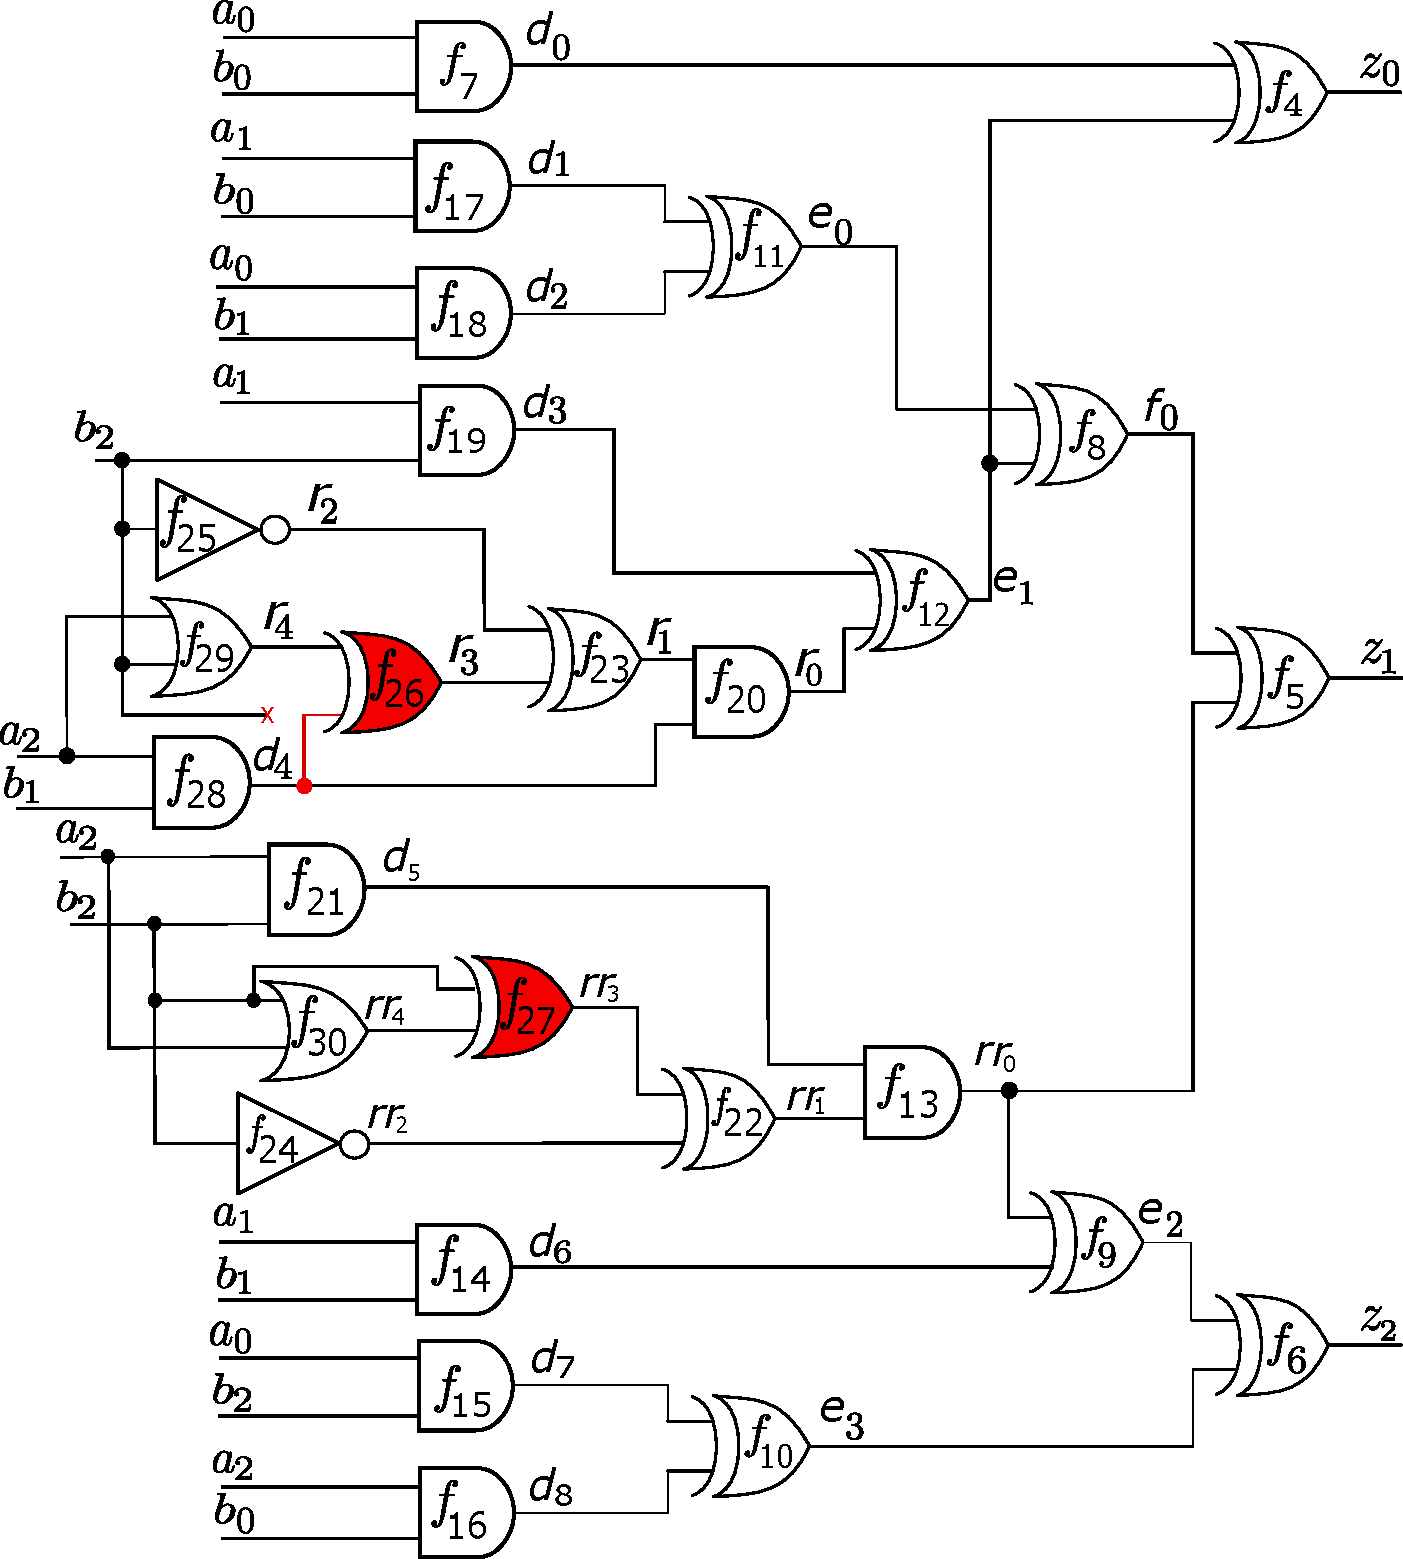
\includegraphics[scale=0.26]{mas_3_ddc_mfr_a.pdf}
\caption*{A faulty implementation of a 3-bit modulo multiplier ($Z = A \cdot B~~mod~P(x)$)
% ($n$=3) with gate replacement bugs introduced at nets $d_5$ (AND replaced with an OR) and $d_2$ (AND replaced with an XOR), and a wire replacement bug at net $e_0$ (input shorted to $d_0$ instead of $d_1$).
}\label{fig:mas_bug_Wa}
\end{figure}
\end{frame}


\begin{frame}{\large Problem Description: Rectification}
\bi 
	% \item Identify rectification target nets
	% \bi
	% 	\item Post-verification failure analysis
	% 	\item Primary output always a candidate for a correction
	% \ei
	\item Agnostic to the fault model, check for rectification at particular targets
	\bi
	\pause
		\item Single-fix Rectification (SFR)
		\bi
			\item Correct circuit by changing function at a single net
		\ei
	\ei
	\pause
	\vspace{0.1in}
	\vspace{0.1in}
	\vspace{0.1in}
	\item In a general setting, SFR might not be desired or may not exist
	\bi
	\pause
	\item Multi-fix Rectification (MFR)
	\bi
		\item Correct circuit by changing functions at multiple nets
		\item Contribution: Multi-fix rectifiability setup and check
	\ei
	\ei
\ei
\end{frame}

%https://ieeexplore.ieee.org/document/8405614 - cryptography

% \begin{frame}{\large Motivation: Approximate Computing}

% \bi
% 	\item Trade off accuracy for cost savings [{\it Kulkarni. et al}, VLSI'11]
% 	\item Synthesize approximate circuit by performing ECO style patch on original exact circuit
% \ei
% %\item Application to approximate circuits
% % \bi
% % 	\item Exact efficient implementation given
% % 	\item Rectify it minimally to match a new approximate $spec$
% % \ei
% \begin{figure}[hbt]
% \centering
% 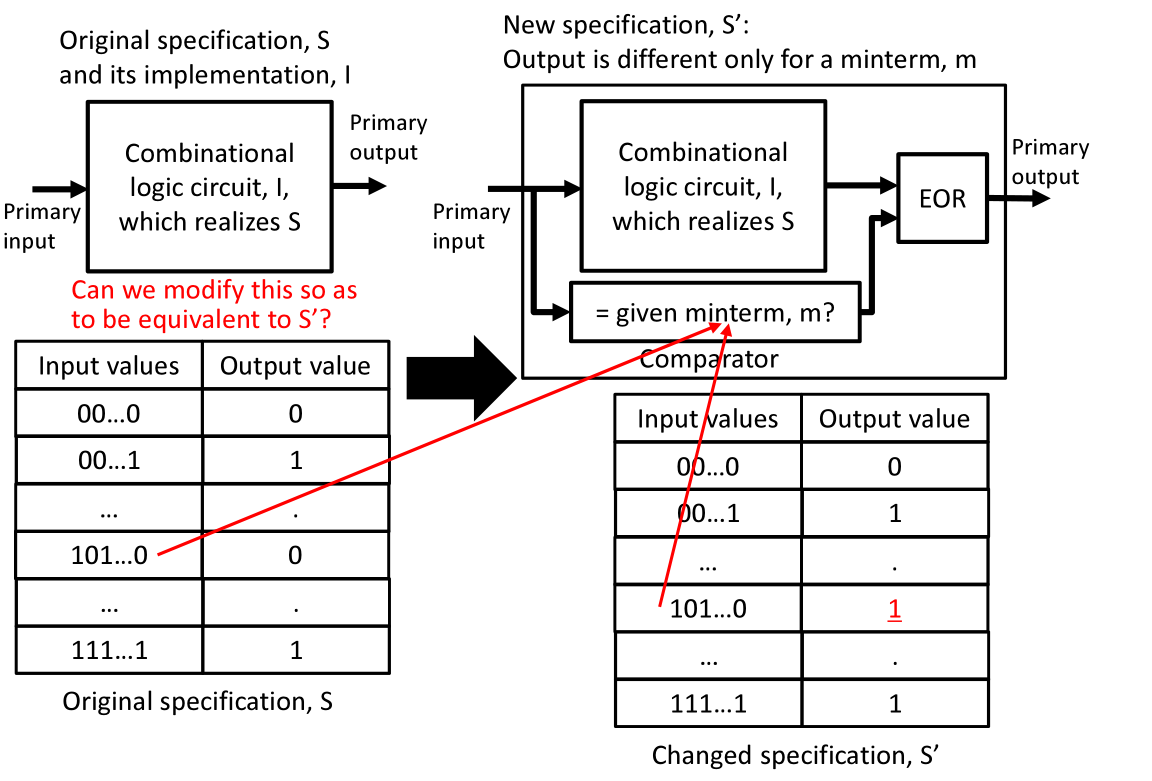
\includegraphics[scale = 0.25]{minterm.png}
%     \caption{Single minterm functional change. EOR = Ex-OR gate}
%     \label{fig:mint}
% \end{figure}
% \end{frame}

% \begin{frame}{\large Focus: Integer Arithmetic Circuits}
% \bi
% 	\item Approximate integer primitives
% 	\bi
% 		\item Exploits error resilience of real-world applications
% 		\item Neuromorphic Architectures, Data mining, Machine Learning, etc.
% 		\item Quantification:
% 		\bi
% 			\item Magnitude: Maximum deviation of the approximate output as
% compared to the defined constraint
% 			\item Frequency: Ratio of the number of magnitude deviations from the correct
% value to the total number of outputs
% 		\ei
% 	\ei
% 	\vspace{0.1in}
% 	\item {\it Lamb} investigated SFR of approximate integer multipliers
% 	\bi
% 		\item Single cube error (frequency) introduced across two output bits (magnitude)
% 		% \bi
% 		% 	\item Translates to corruption of a single minterm entry in the original truth table for respective outputs
% 		% \ei
% 		% \item Observations from experiments on 2/3/4-bit multiplier circuits
% 		\bi
% 			\item {\red 4\%} of 2-bit, {\red 1.6\%} of 3-bit approximate specs admits SFR
% 			\item 4-bit circuit has {\red zero} SFR points
% 		\ei
% 	\ei
% \ei
% \end{frame}



% \begin{frame}{\large Previous Approaches: Verification}
% \bi
% 	\item Canonical Decision Diagrams
% 	\bi
% 		\item BDDs, BMDs, and their variants
% 		\item Infeasible for arithmetic circuits
% 	\ei
% 	\vspace{0.1in}
% 	\item Combinational Equivalence Checking using SAT
% 	\bi
% 		\item AIG + SAT: Work for structurally similar circuits
% 	\ei
% 	\vspace{0.1in}
% 	\item Verification using computer algebra
% 	\bi
% 		\item Formulations in $\Zkk$: [Namrata et al, TCAD'07]
% 		\item Formulations in $\Fkk$: [Lv et al, TCAD’13] [Pruss et al, TCAD'16]
% 		\item Formulations in $\F_2$: [Cunxi et al, ASP-DAC'17]
% 		\item Integer arithmetic circuits: [Ciesielski et al, DAC'15] [A.Sayed et al, DATE’16] [D. Ritirc et al, FMCAD’17]
% 		[A. Sayed et al, FMCAD'16]
% 	\ei
% \ei
% \end{frame}

% \begin{frame}{\large Previous Approaches: Rectification}
% % Ideas came from ATPG, Boolean Differences, 
% % Based on Boolean reasoning engines
% % Then SAT solvers became efficient and replaced those
% % SAT based decision procedure for rectification test 
% % if it passes, the way the problem is set-up Craig interpolants
% % can be used to compute the rf
% % 12 bit: then we started looking into this problem. Our group has
% % already done on verification using computer algebra which is
% % scalable on FF ckts, from there we started looking into rectification using this formulation
%!TEX root = UG_PhD_Defense.tex
\begin{frame}{\large Preliminaries: Finite field basics}
\bi
	\item Fields - set of elements over which operations $(+,\cdot,/)$ can be performed 
	\bi
		\item Ex. $\R,\Q,\C$
	\ei
	\vspace{0.1in}
	\item Finite fields (Galois fields) - Finite set of elements
	\bi
		\item Ex. $\F_q$, where $q=p^n,~p~=~prime,~n \in \Z_{\geq 1}$ 
		\bi
		\item When $n=1$, $\F_p = \Z_p \pmod{p}$
		\item With $p=2$, $\F_2 = \B = \{0,1\}$
		\ei
		\item On circuits, $p=2$, $n=$ data-operand width
	\ei
	\vspace{0.1in}
	\item Hardware cryptography extensively based on $\Fkn$ (we use $\Fkn$)
    % \bi
		% \item $\F_2 \subset \Fkn$, $n>1$
	% \item We are interested in fields of type $\Fkn$
	% \bi
	% 	\item Binary Galois extension fields with characteristic $2$ ($p$)
	% 	\bi
	% 		\item 
	% 		\item Bit-vector of size $n$ represents $2^n$ distinct elements
	% 	\ei
	% 	\item Finite field properties allow elegant application of algebraic geometry techniques
		% \bi
		% 	\item Practical applications to hardware design, debug, verification, and rectification
		% \ei
	% \ei
\ei
\end{frame}

\begin{frame}{\large Preliminaries: Modeling circuit polynomials over $\Fkn$}
\bi
	\item Boolean logic gates in $\F_2 ~~(\F_2 \subset \Fkn)$. Over $\F_2$, $-1=+1\pmod{2}$
\ei
	\begin{align*}
		 z &=~ \sim a &\implies &z+a+1 &\pmod{2}\\
		 z &= a \wedge b &\implies &z+a\cdot b &\pmod{2}\\
		 z &= a \vee b &\implies &z+a\cdot b + a + b &\pmod{2}\\
		 z &= a \oplus b &\implies &z+a+b &\pmod{2}
	\end{align*}

\bi
	\item Word-level polynomials [$\ga$ = primitive element of $\Fkn$]
\ei
\begin{equation*}
\begin{split}
 Output:  Z + z_0 +\gamma \cdot  z_1 + \dots +\gamma^{n-1} \cdot z_{n-1}\\
 Input:  A + a_0 +\gamma \cdot a_1 + \dots +\gamma^{n-1} \cdot a_{n-1}
\end{split}
\end{equation*}
\end{frame}

\begin{frame}{\large Problem Statement and Objective}
\bi
	\item A multivariate specification polynomial $f \in \Fkn$
	\bi
		\item $n$ is the operand width
		\item Ex. $Z = A \cdot B \pmod{P_n(x)}$ over $\Fkn$
	\ei 
	\vspace{0.1in}
	\item A faulty circuit implementation $C$ for specification $f$ 
	\bi
		\item Model gates as polynomials over $\Fkn$
	\ei
	\vspace{0.1in}
	\item A primitive polynomial $P_n(x)$ used to construct $\Fkn$
	\bi
		\item $\Fkn$ constructed as $\Fkn = \F_2[x] \pmod{ P_n(x)}$
		\item Let $\ga$ be one of the roots of $P_n(x)$, i.e. $P_n(\ga) = 0$
	\ei
	 % , s.t. $P_n(\ga) = 0$
	\vspace{0.1in}
	\item A set of $m$ targets from $C$ (modeled over $\Fkm$)
	\vspace{0.1in}
	\vspace{0.1in}
	\item Check if $C$ is rectifiable at these $m$ targets 


\ei
\end{frame}



\begin{frame}{\large Algebraic Geometry: Ideals}
\bi
	\item Let $R=\ftnwring$
	\bi
		\item $\{f_1, \dots, f_s\} \in R$
	\ei
	\vspace{0.1in}
	\item In our context
	\bi
		\item $x_1,\dots,x_d$: Variables (nets of the circuit)
		\item $Z$: bit-vector representation for variables
		\item $f_1, \dots, f_s$: Polynomials from the circuit (logic gate relations)
	\ei
	\vspace{0.1in}
	\item $J = \langle F \rangle = \langle f_1, \dots, f_s \rangle \subseteq R$
	\bi
		\item $\{h_1f_1 + \cdots + h_sf_s:~h_i \in R\}$
		\item Polynomials $f_1, \dots, f_s$: {\it basis} or {\it generators} of $J$
	\ei
	\vspace{0.1in}
	\item Vanishing Ideal: $J_0 = \langle F_0 \rangle =  \langle x_1^2+x_1,\dots,x_d^2+x_d, Z^{2^n}+Z\rangle$
	\bi
		\item Restrict solutions to $x_i$ in $\F_2$, and solutions to $Z$ in $\Fkn$
	\ei
\ei
\end{frame}

\begin{frame}{\large Algebraic Geometry: Varieties}
\bi
	% \item Let $J = \langle F \rangle = \langle f_1, \dots, f_s \rangle \subseteq R=\ftnwring$
	% \vspace{0.1in}
	% \item Vanishing Ideal: $J_0 = \langle F_0 \rangle =  \langle x_1^2+x_1,\dots,x_d^2+x_d, Z^{2^n}+Z\rangle$
	\item $J = \langle F \rangle = \langle f_1, \dots, f_s \rangle \subseteq \ftnwring $
	\vspace{0.1in}
	\item Let $\bm{a} = (a_1,\dots,a_d) \in \Fkn^d$ $s.t.$ $f_1(\bm{a}) = \cdots = f_s(\bm{a})=0$
\ei
\begin{align*}
V(J) = \text{Set of all }\{\bm{a}\} \text{ s.t. }\begin{cases}
f_1(\bm{a}) = 0, \\
f_2(\bm{a}) = 0, \\
\vdots \\
f_s(\bm{a}) = 0
\end{cases}
\end{align*}
\bi
\item $V(J)$ correspond to function mappings (Truth tables)
\ei
\end{frame}

\begin{frame}{\large \Grobner Basis and Ideal membership}
\bi
	\item An ideal $J = \langle f_1,\dots,f_s\rangle \subseteq R$ can have many generators. 
	\bi
		\item $J = \langle p_1,\dots,p_m\rangle = \dots = \langle g_1,\dots,g_t\rangle$
		\item \Grobner Basis (GB) is one such set with special properties
		% \bi
		% 	\item Presence or absence of solutions (varieties)
		% 	% \item Determine dimension of varieties.
		% 	\item Ideal membership of a polynomial
		% \ei
	\ei
	% \bi
	% 	\item Same ideal different sets of generators
	% \ei
	% \vspace{0.1in}
	
	\vspace{0.1in}
	\item Let $J =  \langle f_1,\dots,f_s\rangle = \langle g_1,\dots,g_t\rangle$
	and $G = GB(J) = \{g_1,\dots,g_t \}$.
	\bi
	\item $G$ is a \Grobner basis of $J \iff \forall f \in J, f \xrightarrow[]{g_1,\dots,g_t}_+ 0$ 
	% \ei
	% \vspace{0.1in}
	\item Ideal membership: Let $f$ be a polynomial in $R$:
	\bi
		\item if $f \xrightarrow[]{g_1,\dots,g_t}_+ 0$, then $f$ is a member of $J$. 
	\ei
	\ei
\ei
\begin{figure}
\centering
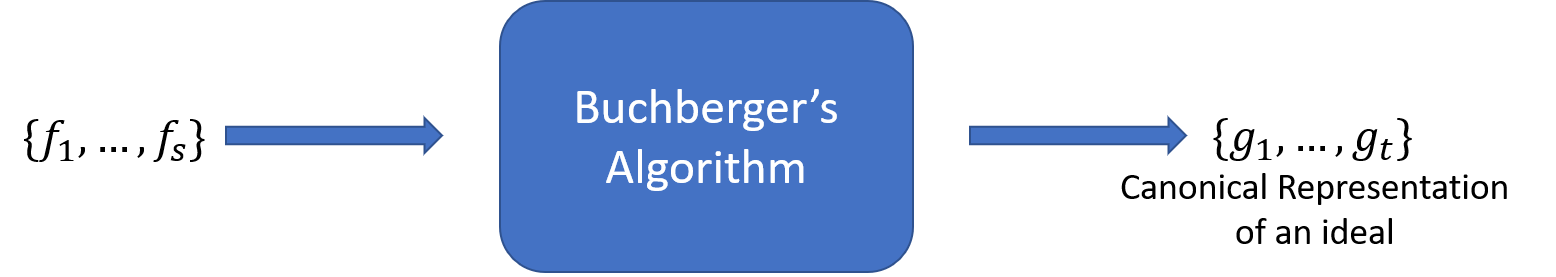
\includegraphics[scale=0.39]{GB.png}
\end{figure}
\end{frame}

% \begin{frame}{\large Extended \Grobner Basis}

% \bi
% \item Helps relate an ideal with any generating set contained in the ideal

% %\begin{center}
% \begin{equation*}\label{eqn:matrix}
% \begin{bmatrix} g_1 \\ g_2 \\ \vdots \\ g_t \end{bmatrix}  =  M \cdot
% \begin{bmatrix} f_1 \\ f_2 \\ \vdots \\ f_s \end{bmatrix}
% \end{equation*}
% \item M is a $t\times s$ matrix of polynomials

% \item if $f \in J$, then
% \bi
% \item $f = u_1g_1 + u_2g_2+ \dots+ u_tg_t$
% \item $f = v_1f_1 +\dots+v_sf_s$
% \ei
% \item Used in computation of rectification function
% \ei
% \end{frame}


%How are two ideals and their varieties related? 
%Analyzing Ideal 𝐽 is not enough Need to analyze ideal 𝐼(𝑉( 𝐽))
%SNS reasons about the ideal of polynomials that vanish on V(J).


% \begin{frame}{\large Strong Nullstellensatz}
% \bi
% \item Given an ideal $J\subset R$ and $V(J) \subseteq \Fq^d$ 
% % the {\it ideal of polynomials that vanish on} $V(J)$ is 
% \bi
% 	\item $I(V(J)) = \{ f \in R : \forall \bm{a} \in V(J), f(\bm{a}) = 0\}$.
% \ei

% \item If $f$ vanishes on $V(J)$, then $f \in I(V(J))$. 

% \item The Strong Nullstellensatz characterizes $I(V(J))$ over $\Fq$
% \bi
% 	\item Over finite fields $\Fq$, $I(V_{\Fq}(J)) = J + J_0$.
% 	\item We will use this to formulate rectification check
% \ei
% \ei
% \end{frame}
%!TEX root = UG_PhD_Defense.tex
%Single-fix Rectification
%Show our current progress on single fix rectification
%redundancy?

% \begin{frame}{\large Single-fix Rectification: Prior work}
% \bi
% 	\item Automated Diagnosis: Boolean Reasoning [{\it Madre. et al}, ICCAD'89] [{\it Liaw. et al}, ICCAD'90]
% 	\item Engineering Change Order (ECO): CNF-SAT formulation
%  	[{\it Marek-Sadowska. et al}, DAC'95] [{\it Huang. et al}, ICCAD'10] 
%  	\item Partial Synthesis: Quantified Boolean Formula(QBF)
%  	[{\it Scholl. et al}, ICCD'13] [{\it Fujita. et al}, Proc IEEE'15]
%  	\item Symbolic Computer Algebra techniques:
%  	\bi
%  		\item Rectification of finite field circuits [{\it Rao. et al}, FMCAD'18][{\it Gupta. et al}, VLSI-SOC'18]
%  		\item  Automated Debugging of integer arithmetic circuits using Computer Algebra
% 			[{\it Mishra. et al}, ICCD'17] [{\it Mishra. et al}, DATE'16] [{\it Ciesielski. et al}, DAC'15]
% 			% \bi
% 			% \item Incorrect and incomplete: Approach heavily relies on the structure of the circuit
% 			% \ei
%  	\ei
% \ei
% \end{frame}

\begin{frame}{\large Application: Single-Fix Rectification}
% \begin{columns}
% 	\begin{column}
		\begin{figure}[hbt]
		\centering
		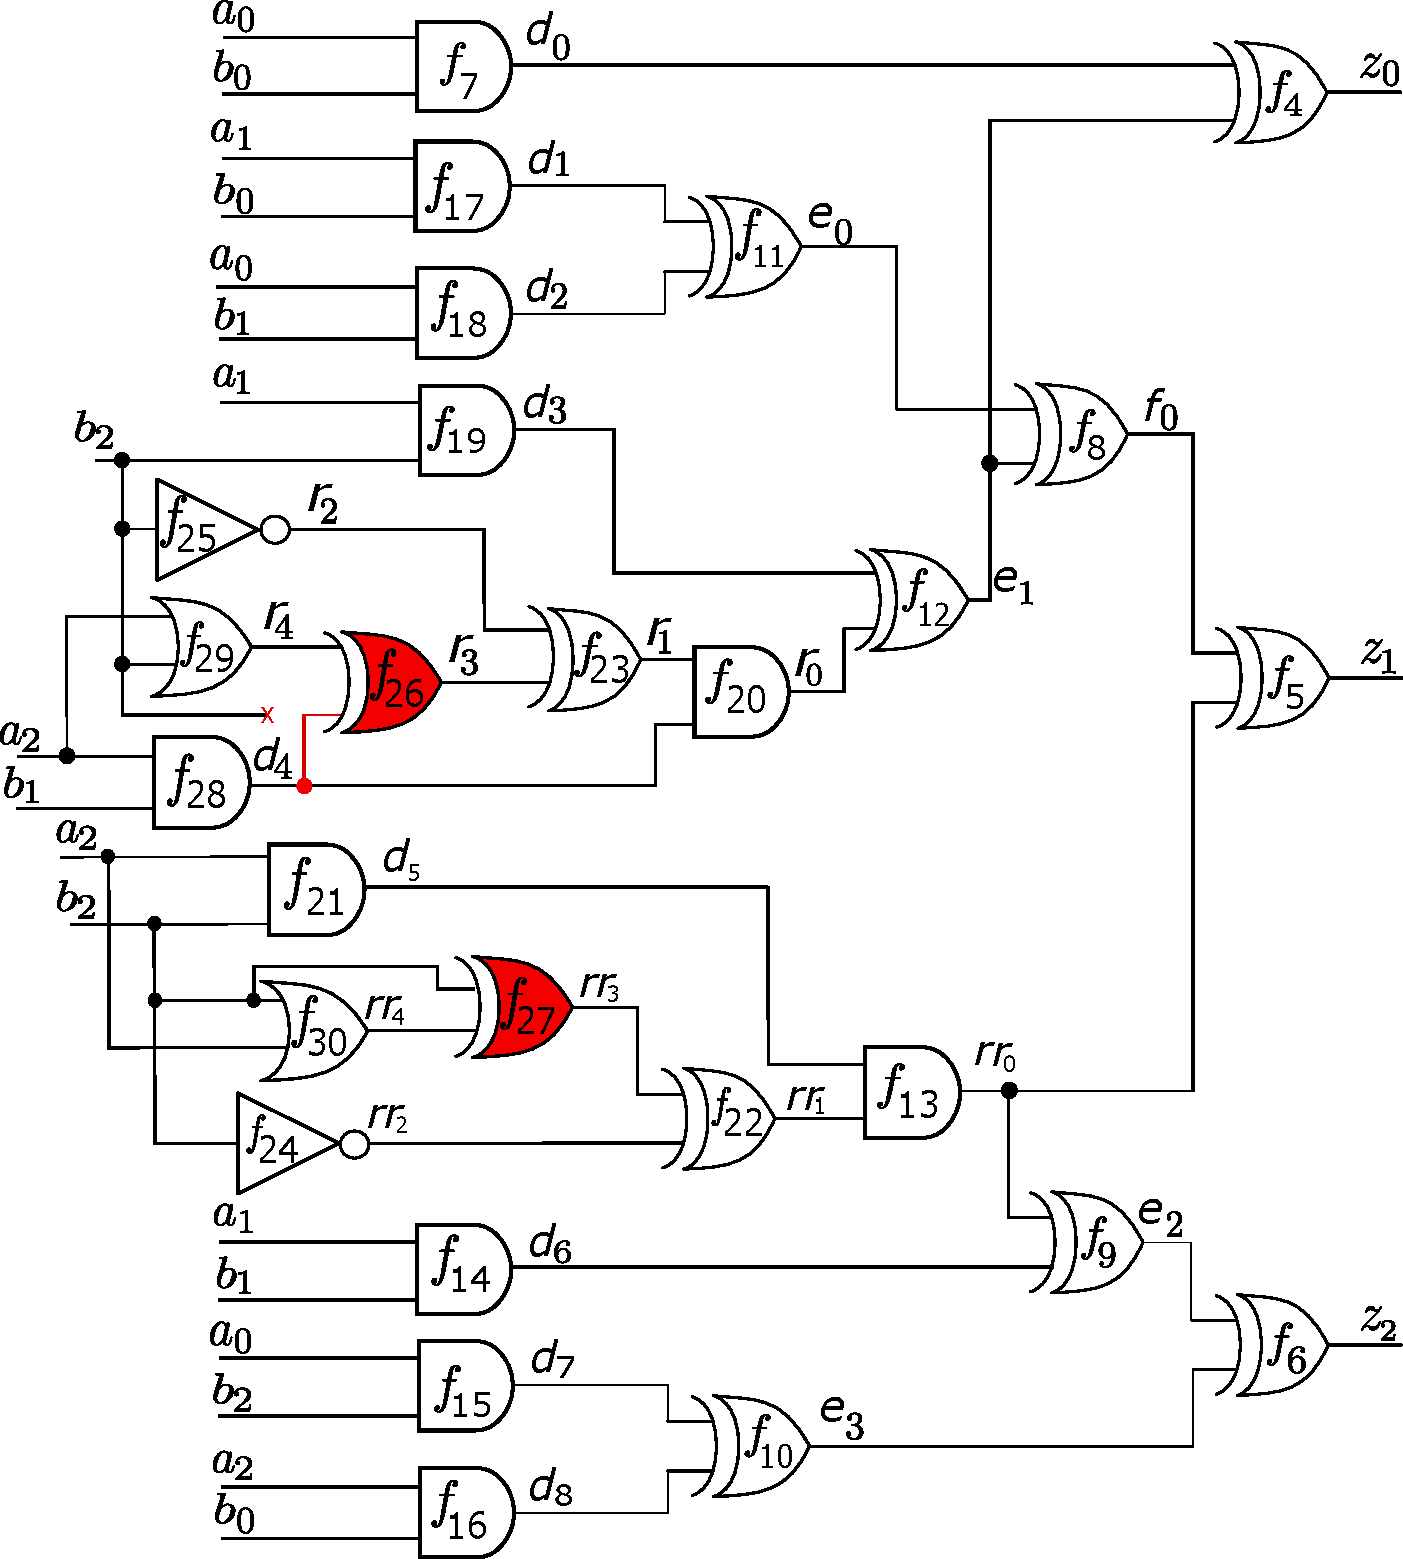
\includegraphics[scale=0.26]{mas_3_ddc_mfr_a.pdf}
		\caption*{A faulty implementation of a 3-bit modulo multiplier ($Z = A \cdot B~~mod~P_3(x)$)
		% ($n$=3) with gate replacement bugs introduced at nets $d_5$ (AND replaced with an OR) and $d_2$ (AND replaced with an XOR), and a wire replacement bug at net $e_0$ (input shorted to $d_0$ instead of $d_1$).
		}\label{fig:mas_bug_ca}
		\end{figure}
% 	\end{column}

% 	\begin{column}
% 	\bi
% 	\item Impose RTTO $>$
% 	\ei
% 	\begin{small}
% 		\begin{flalign*}
% 		f_1:Z + z_0 +\ga \cdot z_1 + \ga^2 \cdot z_2;\\
% 		f_2:A + a_0 +\ga \cdot a_1 + \ga^2 \cdot a_2;\\
% 		f_3:B + b_0 +\ga \cdot b_1 + \ga^2 \cdot b_2;\\
% 		f_4:z_0 + d_0 + e_1;   \\             		
% 		f_5:z_1 + f_0 + rr_0;   \\            		
% 		\dots  \\
% 		f_{22}:rr_1 + rr_3+rr_2; \\
% 		f_{23}:r_1 + r_2+r_3;\\
% 		\red{f_{26}:r_3 + r_4 + d_4;}\\
% 		{\red f_{27}:rr_3 + rr_4 + b_2;}\\
% 		\dots\\
% 		f_{30}:rr_4 + a_2+b_2+a_2b_2;                             		
% 		\end{flalign*}
% 	\end{small}
% 	\end{column}
% \end{columns}
\end{frame}

\begin{frame}{\large Preliminaries: Term order}
\bi
	\item Reverse Topological Term Order (RTTO)
	\bi
		\item Exploit circuit structure to avoid expensive GB computation
		\item Standard practice to order variables topologically from POs to PIs
	\ei
	\pause
	\vspace{0.1in}
	\item Impose RTTO $>$ on circuit $C$:
	\begin{small}
\begin{flalign*}
f_1:Z + z_0 +\ga \cdot z_1 + \ga^2 \cdot z_2;   &\quad f_{22}:rr_1 + rr_3+rr_2; \\
f_2:A + a_0 +\ga \cdot a_1 + \ga^2 \cdot a_2;   &\quad f_{23}:r_1 + r_2+r_3;\\
f_3:B + b_0 +\ga \cdot b_1 + \ga^2 \cdot b_2;   &\quad \red{f_{26}:r_3 + r_4 + d_4;}\\
f_4:z_0 + d_0 + e_1;                &\quad {\red f_{27}:rr_3 + rr_4 + b_2;}\\
f_5:z_1 + f_0 + rr_0;               &\quad \dots\\
\dots                               &\quad f_{30}:rr_4 + a_2+b_2+a_2b_2;
\end{flalign*}
\end{small}
\pause
\vspace{-0.1in}
\item $F = \{f_1,\dots,f_{30}\}$, $F_0 =\{a_0^2-a_0,\dots,z_2^2-z_2,A^8-A,\dots,Z^8-Z\}$. 
\bi
	\item Ideal $J+J_0=\langle F\cup F_0\rangle$ models $C$.
\ei
\ei

\end{frame}

\begin{frame}{\large Application: Single-Fix Rectification}
\bi
	\item Denote polynomial $f: Z + A\cdot B$ as the design specification.
	\vspace{0.1in}
	\pause
	\item Ideal $J+J_0=\langle F\cup F_0\rangle$ representing circuit $C$.
	\vspace{0.1in}
	% \pause
	% \item $F = \{f_1,\dots,f_{30}\}$, $F_0 =\{a_0^2-a_0,\dots,z_2^2-z_2,A^8-A,\dots,Z^8-Z\}$. 
%under RTTO $>$, $F\cup F_{0}$ constitutes a GB of
	\vspace{0.1in}
	\pause
	\item Circuit designed over $\Fkn = \F_{2^3} (n=3)$ using 
	$P_n(x) = P_3(x) = x^3+x+1$ with $P_3(\ga)=0$

	\vspace{0.1in}
\pause
\item {\bf Is this circuit rectifiable at net $r_3$?}
\ei


% \begin{figure}[hbt]
%     \begin{center}
%     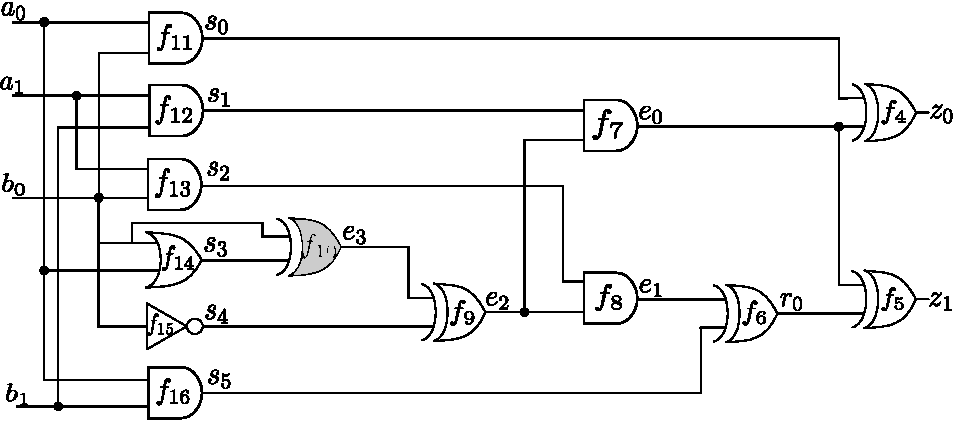
\includegraphics[scale = 0.64]{mas_red_bug-eps-converted-to.pdf}
%     \end{center}
% %    \vspace{-4ex}
%     \caption*{\small A 2-bit faulty modulo
%       multiplier implementation. 
%     %   with the bug at
%     % net $e_3$. A correct implementation will have an AND gate at $e_3$,
%     % which has been replaced by an XOR gate.
%     }
%     \label{fig:mas_both}
% \end{figure}

\end{frame}

% \begin{frame}{\large SFR Application: Verification}
% \bi

% 	\item Denote polynomial $f: Z + A\cdot B$ as the design specification.
% 	\item Impose RTTO $>$
% \ei
% \[ \begin{array}{lll}%									   
% f_1:Z + z_0 +\ga \cdot z_1;&\quad  f_7:e_0 + s_1e_2; 	   &\quad f_{12}:s_1 + a_1b_1; \\
% f_2:A + a_0 +\ga \cdot a_1;&\quad  f_8:e_1 + s_2e_2; 	   &\quad f_{13}:s_2 + a_1b_0;  \\
% f_3:B + b_0 +\ga \cdot b_1;&\quad  f_9:e_2 + e_3 + s_4;    &\quad f_{14}:s_3 + a_0 + b_0 + a_0b_0; \\ 
% f_4:z_0 + s_0 + e_0;  	   &\quad  \alert{f_{10}:e_3 + b_0 + s_3;} &\quad f_{15}:s_4 + b_0 + 1;\\ 
% f_5:z_1 + e_0 + r_0;  	   &\quad  f_{11}:s_0 + a_0b_0;    &\quad f_{16}:s_5 + a_0b_1;  \\
% f_6:r_0 + e_1 + s_5;            						    
% \end{array}\]%

% \bi
% 	\item $F = \{f_1,\dots,f_{16}\}$, $F_0 = \{a_0^2-a_0, a_1^2-a_1,
% b_0^2-b_0, b_1^2-b_1\}$
% 	\item Ideal Membership Test: $f\xrightarrow{F,F_0}_+\ga^1\cdot (a_0a_1b_1b_0+a_0a_1b_1+a_1b_1b_0+a_1b_0) + \ga^0\cdot (a_0a_1b_1b_0+a_0a_1b_1+a_1b_1b_0)$
% \ei
% \end{frame}

% \begin{frame}{\large Application: Single-Fix Rectification}
% \bi
% 	\item Circuit designed over $\Fkn$ using irreducible polynomial $P_n(x) = P_2(x) = x^2+x+1$ with $P_2(\ga)=0$
% \ei
% \begin{figure}[hbt]
%     \begin{center}
%     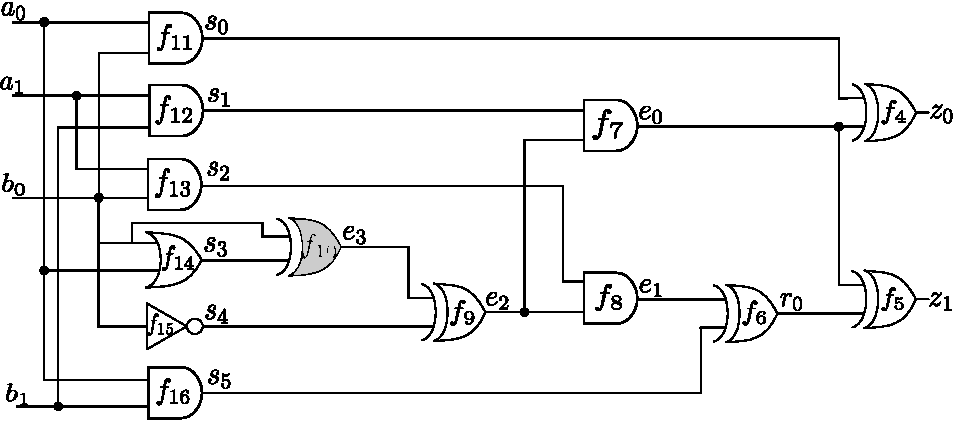
\includegraphics[scale = 0.64]{mas_red_bug-eps-converted-to.pdf}
%     \end{center}
% %    \vspace{-4ex}
%     \caption*{\small A 2-bit buggy modulo
%       multiplier implementation. 
%     %   with the bug at
%     % net $e_3$. A correct implementation will have an AND gate at $e_3$,
%     % which has been replaced by an XOR gate.
%     }
%     \label{fig:mas_both}
% \end{figure}

% \end{frame}

% \begin{frame}{\large SFR Contribution: Identifying Target Nets}
% %We are investigating; and we have some ideas; I will tell you what it is
% %We use a specific order (start from PO); Compute GB with this order; 
% %LEX order eliminates vars; what ends up happening is we get a set of poly
% % in PI and analyze those polynomials; no need to simulation 
% % It's a conjecture that I am targeting; we believe me can formally prove it
% %Suppose we find it; then intersection of cones(figure)
% % Rudimentary approach: If the bug  is observable at multiple outputs, then
% % single-fix rectification is possible at one of the nets 
% % Once GB is computed, the structure of GB is such that
% % we will find exactly one polynomial of the form $t(P)+1$.
% % $P$  

% \begin{figure}
% \centering
% 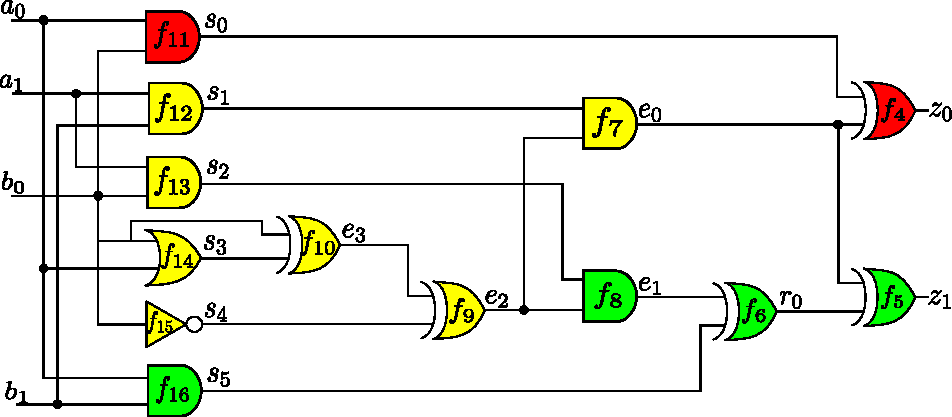
\includegraphics[scale=0.58]{mas_2_bugs_cones.pdf}
% \end{figure}
% \bi
% 	\item Set of affected outputs: $\Oa = \{z_0,z_1\}$
% 	\item Intersection of set of nets in fan-in cones of $\Oa$: $\mN = \{s_4,s_3,s_2,s_1,e_3,e_2,e_0\}$
% 	\item Single-Fix rectification can only exist at a net $x_i \in \mN$
% 	% \item Currently under investigation
% 	% \item Use a specific term order for writing the polynomials
% 	% \item Due to this term-order, GB performs elimination
% 	% \item Analyze polynomials in PI to list POs where error observable
% \ei

% \end{frame}

% \begin{frame}{\large SFR Application: Rectification Check}
% %ATPG V() V() = empty
% %we have an algebraic proof which is there in the proposal
% % \bi
% 	% \item Single-fix rectification exists at net $x_i$, {\it iff} $V_{\Fq}(r_L) \cup V_{\Fq}(r_H) =
%  % 		\Fq^{|X_{PI}|} = V(J_0^{PI}) $
% 	\vspace{0.1in}
% 	% Single-fix patch modeled over $\Fkm = \F_{2} (m=1)$ within a circuit 
% 	% modeled over $\Fkn = \F_{2^2}$
% 	\begin{enumerate}
% 		\item Rectification check at net $e_3$: %$W = \{e_3\}$
% 		\bi
% 			\item $J_1 = \langle F_1\rangle$, where $F_1=\{f_1,\dots, f_{10}=e_3+0,\dots, f_{16}\}$
% 			\item $J_2 = \langle F_2\rangle$, where $F_2 = \{f_1,\dots, f_{10}=e_3+1,\dots, f_{16}\}$
% 		\ei
% 		\vspace{0.1in}
% 		\item Compute $rem_1$ and $rem_2$:
% 		\bi
% 			\item $rem_1 = f \xrightarrow[]{J_1, J_0}_+{(\ga+1)a_1b_1b_0+(\ga+1)a_1b_1}$
% 			\item $rem_2 = f \xrightarrow[]{J_2,J_0}_+{(\ga+1)a_1b_1b_0+(\ga)a_1b_0}$
% 		\ei
% 		\vspace{0.1in}
% 		% \item Single-fix rectification possible iff $G = GB(r1\cdot r2, F_0)=F_0$
% 		\item Single-fix rectification possible iff $V(rem_1) \cup V(rem_2) = \F_{2^2}^{|X_{PI}|} = V(J_0)$
% 		\bi
% 			% \item Compute $G = GB(rem_1\cdot rem_2, J_0)$ and check if $G=J_0$
% 			\item In this example, target $e_3$ admits SFR
% 		\ei
% 	\end{enumerate}
% % \ei
% \end{frame}

\begin{frame}{\large SFR Application: Rectification Check}
%ATPG V() V() = empty
%we have an algebraic proof which is there in the proposal
% \bi
	% \item Single-fix rectification exists at net $x_i$, {\it iff} $V_{\Fq}(r_L) \cup V_{\Fq}(r_H) =
 % 		\Fq^{|X_{PI}|} = V(J_0^{PI}) $
	\vspace{0.1in}
	% Single-fix patch modeled over $\Fkm = \F_{2} (m=1)$ within a circuit 
	% modeled over $\Fkn = \F_{2^2}$
	\begin{enumerate}
		\item Rectification check at net $r_3$: %$W = \{e_3\}$
		\bi
			\item $J_1 = \langle F_1\rangle$, where $F_1=\{f_1,\dots, f_{26}=r_3+0,\dots, f_{30}\}$
			\item $J_2 = \langle F_2\rangle$, where $F_2 = \{f_1,\dots, f_{26}=r_3+1,\dots, f_{30}\}$
		\ei
		\vspace{0.1in}
		\pause
		\item Compute $rem_1$ and $rem_2$:
		\bi
			\item $rem_1 = f \xrightarrow[]{J_1, J_0}_+{(\ga+1)\cdot a_2b_1b_2+(\ga^2+\ga)\cdot a_2b_2}$
			\item $rem_2 = f \xrightarrow[]{J_2,J_0}_+{(\ga+1)\cdot a_2b_1b_2+(\ga+1)\cdot a_2b_1+(\ga^2+\ga)\cdot a_2b_2}$
		\ei
		\vspace{0.1in}
		\pause
		% \item Single-fix rectification possible iff $G = GB(r1\cdot r2, F_0)=F_0$
		\item SFR possible {\bf iff} $V(rem_1) \cup V(rem_2) = \F_{2^3}^{|X_{PI}|} = V(J_0)$
		\bi
		\pause
			\vspace{0.1in}
			\item Compute $G = GB(rem_1\cdot rem_2, J_0)$ and check if $G=J_0$
			\vspace{0.1in}
			\item In this example, target $r_3$ doesn't admit SFR
		\ei
	\end{enumerate}
% \ei
\end{frame}


% \begin{frame}{\large SFR Application: Computing Rectification Function}
% \bi
% 	\item Rectification check confirmed there exists a polynomial at net $e_3$: $f_{10}: e_3 + U$ that can
% 	rectify the circuit. 
% 	\bi
% 		\item Here $U$ is the \textit{unknown component} to be computed.
% 	\ei
% 	\item Update $F$ to $F=\{f_1,\dots,f_{10} = e_3+U,\dots,f_{16}\}$
% 	\item For a correct implementation, $f\xrightarrow{F\cup F_{0}^{PI}}_+0$ still holds
% 	\item Obtain the remainder $r$ and quotient of division $h_{10}$ as:
% 	\bi
% 		\item $f\xrightarrow[]{{f_1}}\dots\xrightarrow[]{{e_3}}[\underbrace{{(\ga+1)s_1+\ga s_2}}_\text{$h_{10}$}]({e_3})+\{\underbrace{{\scriptstyle s_0+(\ga+1)s_1s_4+\ga s_2s_4+\ga s_5+\ga a_0b_1+a_0b_0+(\ga+1)a_1b_1+\ga a_1b_0\}}}_\text{$r$}$
% 	\ei
% 	\item The \textit{unknown component} problem is then formulated as an ideal membership test and
% 	solved using extended \Grobner Basis: 
% 	\bi
% 		\item $r \in \langle h_{10},f_{11},f_{12},f_{13},f_{14},f_{15},f_{16}\rangle
% 	  		+ \langle F_{0}^{PI}\rangle$.
% 		\item $U=b_0$, i.e. $f_{10} = e_3 + b_0$
% 	\ei
% \ei
% \end{frame}

\begin{frame}{\large Unified framework motivation}
\bi
	\item For Single-fix, $m=1$
	\bi
		\item Rectification patch modeled over $\Fkm = \F_{2^1} = \F_2$
		\item Circuit modeled over $\Fkn$ 
		\pause 
		\bi
		    \item $\forall n \in \Z_{>1}$, $1 \mid n$, $\F_2 \subset \F_{2^n}$, 
		\ei
	\ei
	\pause
	\vspace{0.1in}
	\item For Multi-fix, since $m > 1$, $\Fkm$ might not be contained in $\Fkn$
	\bi
		\pause
		\item Ex. For $m=2,n=3$, $2 \nmid 3$, $\F_{2^2} \not\subset \F_{2^3}$
	\ei  
	\vspace{0.1in}
	\pause
	\item Composite field $\Fkk$ 
	\bi
		\item $\Fkm \subset \Fkk$ and $\Fkn \subset \Fkk$
	\pause
	\item What are the mathematical challenges?
	\pause
	\item What $P_K(x)$ should be used for constructing $\Fkk$
	\ei
\ei
\end{frame}


% \begin{frame}{\large MFR Contribution: Approach on finite field circuits}
% % \item In a general setting a SFR may not exist even for trivial design bugs in smaller circuits.
% % \bi
% % 	\item Need an approach to address multi-fix rectification
% % \ei
% \bi
% 	\item Checks whether a given circuit $C$ can be rectified at given $m$ targets
% 	% \item Modeling the problem on the lines of SFR may be computationally expensive
% 	\item Word-level formulation
% 	\bi
% 		\item Interpret these $m$ targets as an $m$-bit vector word $W$
% 		\item Our approach aims to test for MFR in a single step
% 		% \item Obviates iterative correction tests, individually, at $m$ targets
% 		\item Multi-fix patch is computed at the bit-vector (word) level in terms of primary inputs: $W=U(X_{PI})$
% 		\bi
% 			\item Function mapping, $f_W:\F_2^n \rightarrow \Fkm$ 
% 			\item Synthesize individual patches from the word-level expression
% 		\ei
% 	\ei
% \ei
% \end{frame}

% \begin{frame}{\large Application: Multi-fix Rectification}
% \begin{figure}[hbt]
% \centering
% 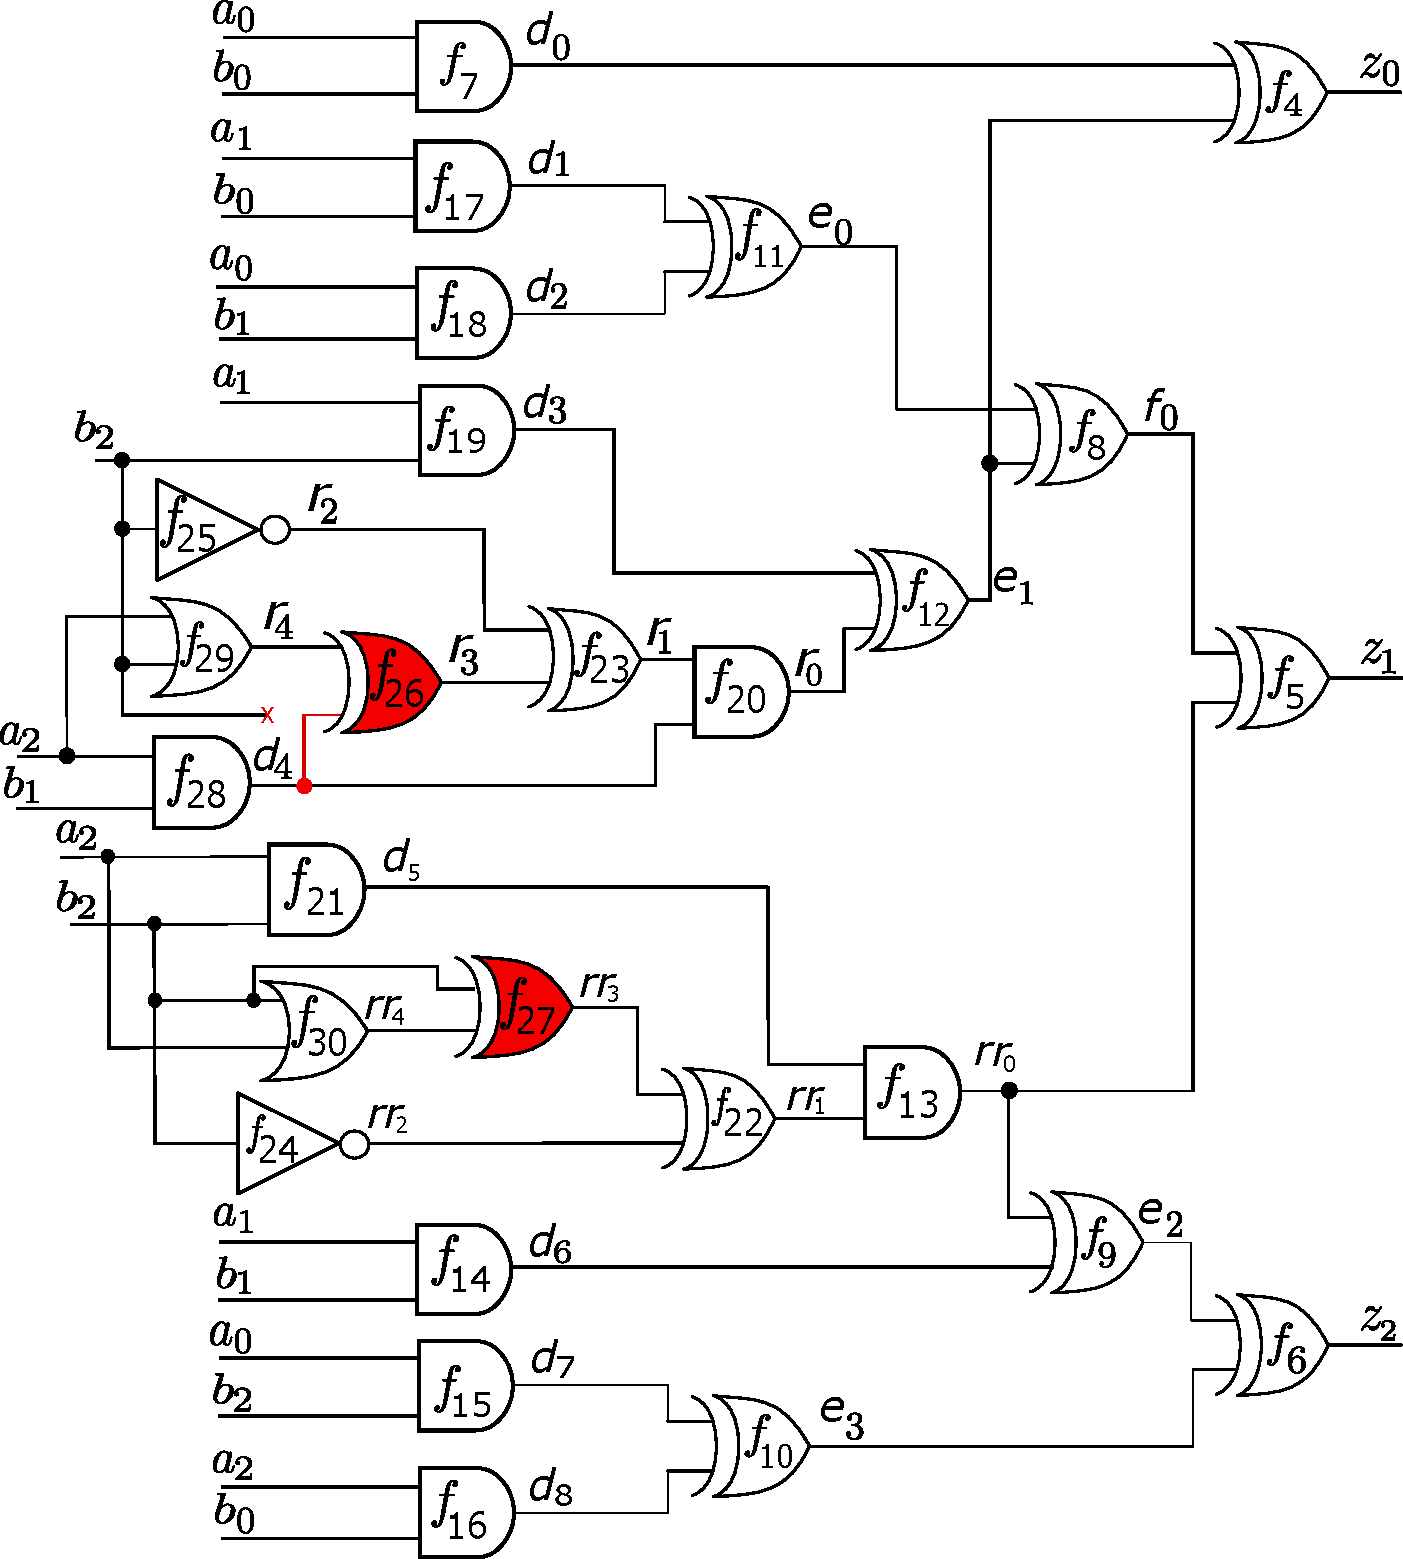
\includegraphics[scale=0.24]{mas_3_ddc_mfr_a.pdf}
% \caption*{A faulty implementation of a 3-bit ($n$=3) Mastrovito multiplier
% % ($n$=3) with gate replacement bugs introduced at nets $d_5$ (AND replaced with an OR) and $d_2$ (AND replaced with an XOR), and a wire replacement bug at net $e_0$ (input shorted to $d_0$ instead of $d_1$).
% }
% \end{figure}
% \end{frame}

% \begin{frame}{\large MFR Application: Polynomial modeling}
% \bi
% 	\item Denote polynomial $f: Z + A\cdot B$ as the design specification.
% 	\item Impose RTTO $>$
% \ei

% \begin{small}
% \begin{flalign*}
% f_1:Z + z_0 +\ga \cdot z_1 + \ga^2 \cdot z_2;   &\quad f_{22}:rr_1 + rr_3+rr_2; \\
% f_2:A + a_0 +\ga \cdot a_1 + \ga^2 \cdot a_2;   &\quad f_{23}:r_1 + r_2+r_3;\\
% f_3:B + b_0 +\ga \cdot b_1 + \ga^2 \cdot b_2;   &\quad \red{f_{26}:r_3 + r_4 + d_4;}\\
% f_4:z_0 + d_0 + e_1;                &\quad {\red f_{27}:rr_3 + rr_4 + b_2;}\\
% f_5:z_1 + f_0 + rr_0;               &\quad \dots\\
% \dots                               &\quad f_{30}:rr_4 + a_2+b_2+a_2b_2;
% \end{flalign*}
% \end{small}

% \bi
% \item $F = \{f_1,\dots,f_{30}\}$, $F_0 =\{a_0^2-a_0,\dots,z_2^2-z_2,A^8-A,\dots,Z^8-Z\}$. 
% %under RTTO $>$, $F\cup F_{0}$ constitutes a GB of
% \item Ideal $J+J_0=\langle F\cup F_0\rangle$ models $C$. 
% \ei
% \end{frame}

% \begin{frame}{\large MFR Notation: Field setup}
% \bi
% 	\item Circuit with data-path size $n$ modeled over $\Fkn$
% 	\bi
% 		% \item Polynomials modeled over $R=\Fkn[Z,A,x_1,\dots,x_d]$
% 		% \bi
% 		% 	\item $\{x_1, \dots$ $, x_d\}$ are all the bit-level variables (nets) in the circuit
% 		% 	\item $Z$ and $A$ are the word-level output and input, respectively
% 		% \ei
% 		\pause
% 		\item $\Fkn = \Ftwo[x]\pmod{P_n(x)}$
% 		\bi
% 			\item $P_n(x) \in \F_2[x]$ is a given degree-$n$ primitive polynomial; $P_n(\ga) =0$ 
% 			% [$\ga$ as one of its root].
% 		\ei
% 		\pause
% 		\item  Word-level polynomials for $Z,A$:
% 		\bi
% 			\item $f_Z: Z + \sum_{i=0}^{n-1}\ga^iz_i,~f_A: A + \sum_{i=0}^{n-1}\ga^ia_i$ 
% 		\ei
% 	\ei 
% 	\vspace{0.1in}
% 	\vspace{0.1in}
% 	\pause
% 	\item Patch size $m$ modeled over $\Fkm$
% 	\bi
% 		\pause
% 		\item $\Fkm = \Ftwo[x]\pmod{P_m(x)}$
% 		\bi
% 			\item We select a degree-$m$ primitive polynomial $P_m(x)\in \F_2[x]$; $P_m(\be) =0$ 
% 			% [$\be$ as one of its root].
% 		\ei
% 		\pause
% 		\item  Word-level polynomial for $W$:
% 		\bi
% 			\item $f_w: W + \sum_{i=0}^{m-1}\be^iw_i$
% 			\item $\{w_0,\dots,w_{m-1}\} \subset \{x_1,\dots,x_d\}$
% 		\ei
% 	\ei
% \ei
% \end{frame}

% \begin{frame}{\large Application: Word-level representation}
% \begin{figure}[hbt]
% \centering
%     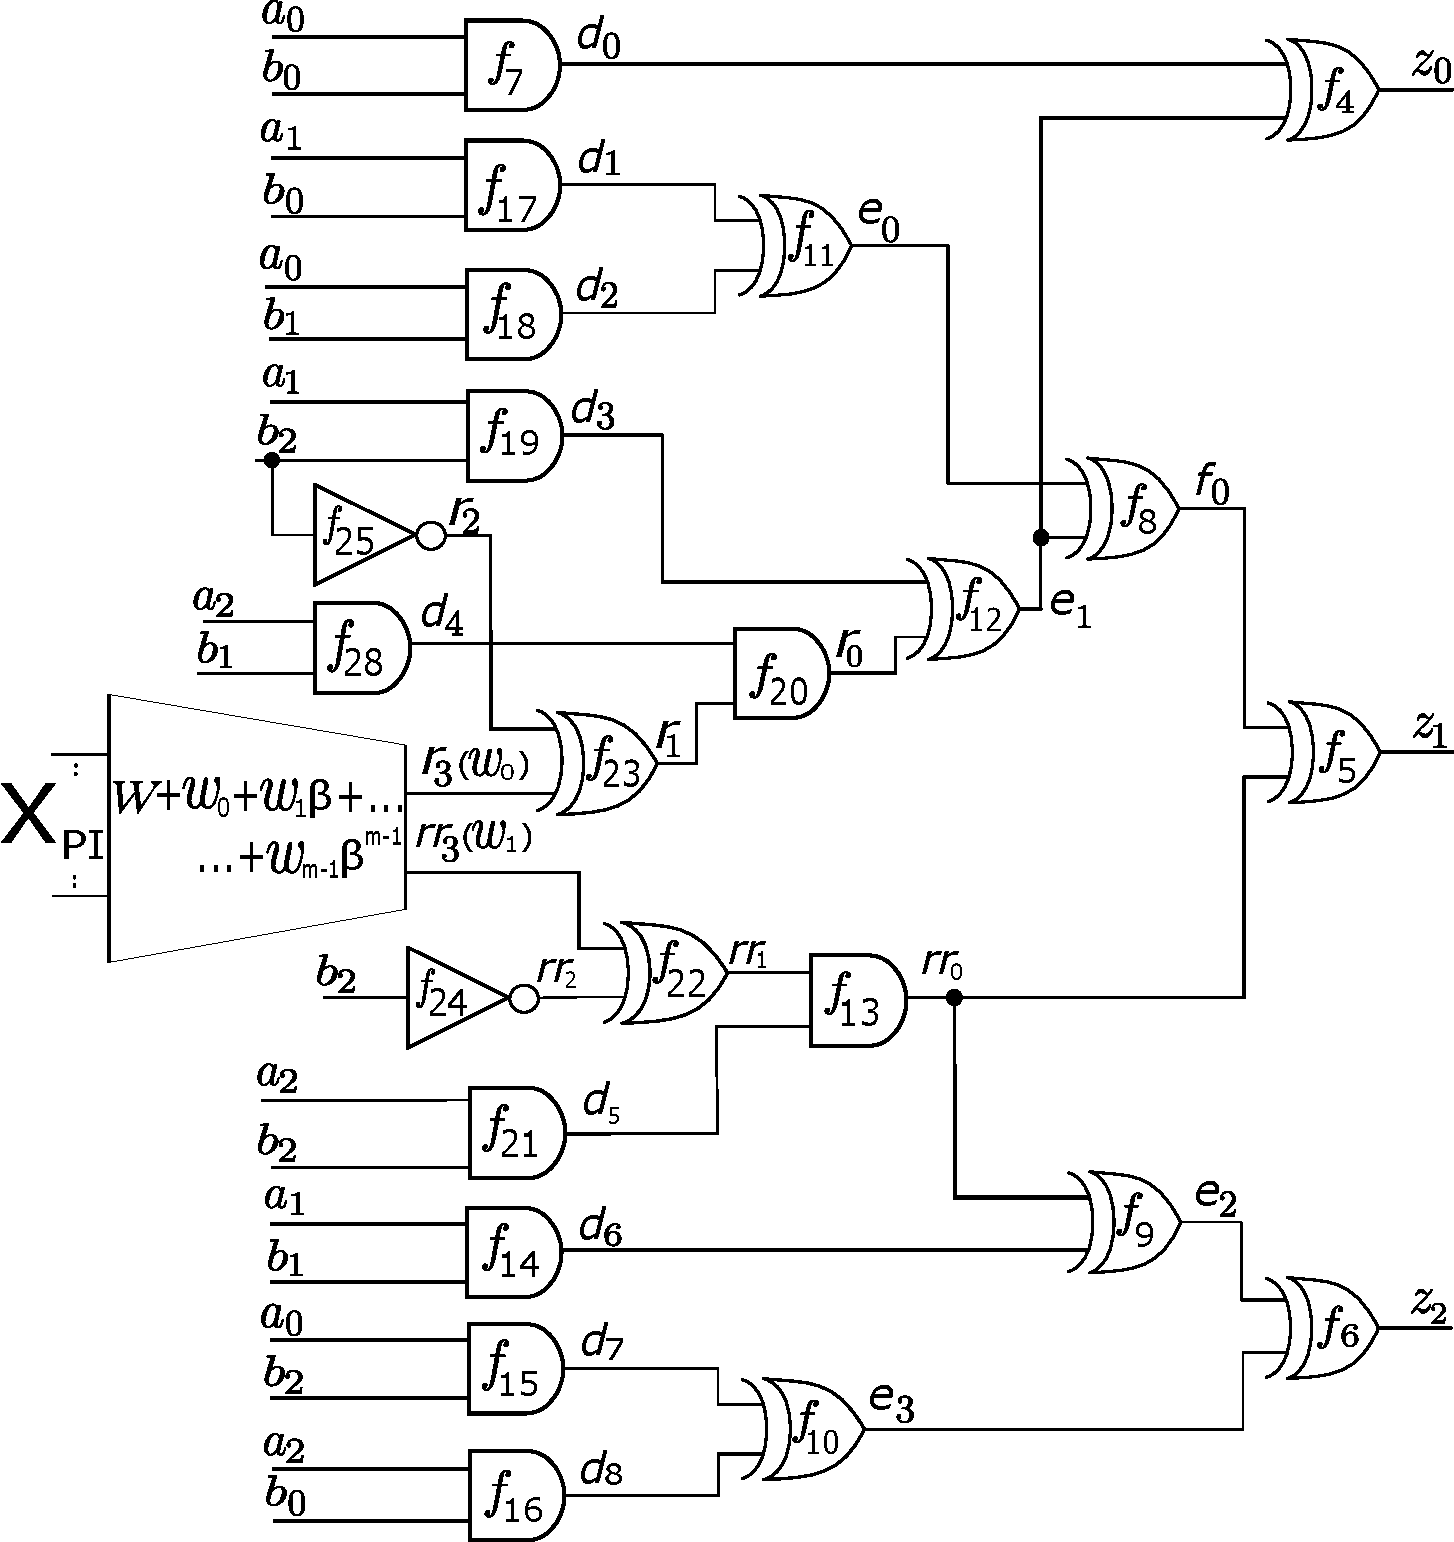
\includegraphics[scale = 0.24]{mas_3_ddc_mfr_b.pdf}
%     \caption*{
%     Patch function modeled as a 2-bit-vector word ($m$=2), 
%     $f_W: W+ r_3 + \beta \cdot rr_3$}
%     \label{fig:mas_bug_W_b}
% \end{figure}
% \end{frame}


% \begin{frame}{\large Mathematical Challenge: Picking $P_k(x)$}
% \bi 

% 	\item Need to represent and manipulate circuit polynomials and the patch function polynomials in one unified domain (composite field)
% 	% \bi
% 	% 	\item How to relate algebraic numbers of lower field to algebraic numbers of higher fields?
% 	% \ei
% 	\vspace{0.1in}
% 	\item Selecting arbitrary $P_k(x)$ leads to erroneous results 
% 	\vspace{0.1in}
% 	\item Solved using Univariate Polynomial Factorization

% \ei
% \end{frame}

\begin{frame}{\large MFR Challenges: $\Fkk$ and $P_k(x)$}
\bi
	% \item Determine the smallest single field ($\Fkk$) to operate both circuit ($\Fkn$) and patch ($\Fkm$)
	% \vspace{0.1in}
	% \item Composite field $\Fkk$ 
	% \bi
	% 	\item $\Fkm \subset \Fkk$ and $\Fkn \subset \Fkk$, $k=LCM(m,n)$
	% \pause
	% \vspace{0.1in}
	% \item What are the mathematical challenges?
	% \pause
	\item Smallest $k$ is $LCM(n,m)$
	\bi
		\vspace{0.1in}
		\item $\Fkk \supset \Fkn$ and $\Fkk \supset \Fkm$
		\vspace{0.1in}
		\item $\Fkk = \Ftwo[x]\pmod{P_k(x)}$
		\bi
			\item $P_k(x)$ is a degree-$k$ primitive polynomial; $P_k(\al) =0$ 
		\ei
	\ei
	\pause
	\vspace{0.1in}

	\item What $P_K(x)$ should be used for constructing $\Fkk$
	\vspace{0.1in}
	\pause
	\item  Mathematical challenge: Given $P_n(x)$ and $P_m(x)$, compute $P_k(x)$ such that
	$P_n(\ga)= P_m(\be)=P_k(\al)=0$
	\pause
	\bi
		\item How are elements $\al$, $\be$, and $\ga$ related?
	\ei
	\vspace{0.1in}
\ei

\end{frame}

% \begin{frame}{\large MFR Notations: Univariate Polynomial factorization (UPF) }
% \bi
% 	\item Given a monic univariate polynomial $f \in \F_q[X]$, where $\F_q$ is any finite field
% 	\vspace{0.1in}
% 	\bi 
% 		\item Find a complete factorization $f = f_1^{e_1}\cdot f_2^{e_2}\cdots f_l^{e_l}$ 
% 		\bi
% 			\item Where $f_1, f_2,\dots, f_l$ are pairwise distinct monic 
% 			irreducible polynomials in $\F_q[X]$ and $e_1,\dots,e_l$ are positive integers.
% 		\ei
% 	\ei
% 	\vspace{0.1in}
% 	% \item We employ existing implementation of UPF from computer algebra tool {\it SINGULAR} 
% \ei
% \end{frame}

\begin{frame}{\large Contribution: Computing $P_k(x)$}
\bi
	\vspace{0.1in}
	\item Property of finite fields, for any element $\phi \in \F_q$, $\phi^{q-1} = 1$
	\vspace{0.1in}
	\pause
	\bi
		\item $\ga = \al^{(2^k-1)/(2^n-1)} = \al^{\lambda}$
		\item $\be = \al^{(2^k-1)/(2^m-1)} = \al^{\mu}$
	\ei
	\pause
	\vspace{0.1in}
	\item Univariate Polynomial Factorization (UPF)
	\pause
	\vspace{0.1in}
	\bi
		\item Obtain UPFs of $P_n(x^{\lambda})$ and $P_m(x^{\mu})$ in $\F_2[x]$
	\ei
	% \bi
	% 	\item Coefficients will be in $\Ftwo$ and degrees will be less than $\lambda$ and $\mu$, respectively.
	% 	\bi
	% 		\item $P_n(x^{\lambda})=P_{n1}^{a1}\cdot P_{n2}^{a2}\cdots P_{nl}^{al}$, and 
	% 		\item $P_m(x^{\mu}) = P_{m1}^{b1}\cdot P_{m2}^{b2}\cdots P_{mg}^{bg}$
	% 	\ei
	% \ei
	\pause
	\vspace{0.1in}
	\item Then, $\exists P_{k}(x) \in \F_2[x]$ as a common factor of $P_n(x^{\lambda})$ and $P_m(x^{\mu})$, such that:
	\bi
		\item $P_{k}(x)$ is a degree-$k$ primitive polynomial in $\F_2[x]$ with $P_k(\al)=0$
	\ei
\ei
\end{frame}

\begin{frame}{\large Application: Word-level representation}
\begin{figure}[hbt]
\centering
    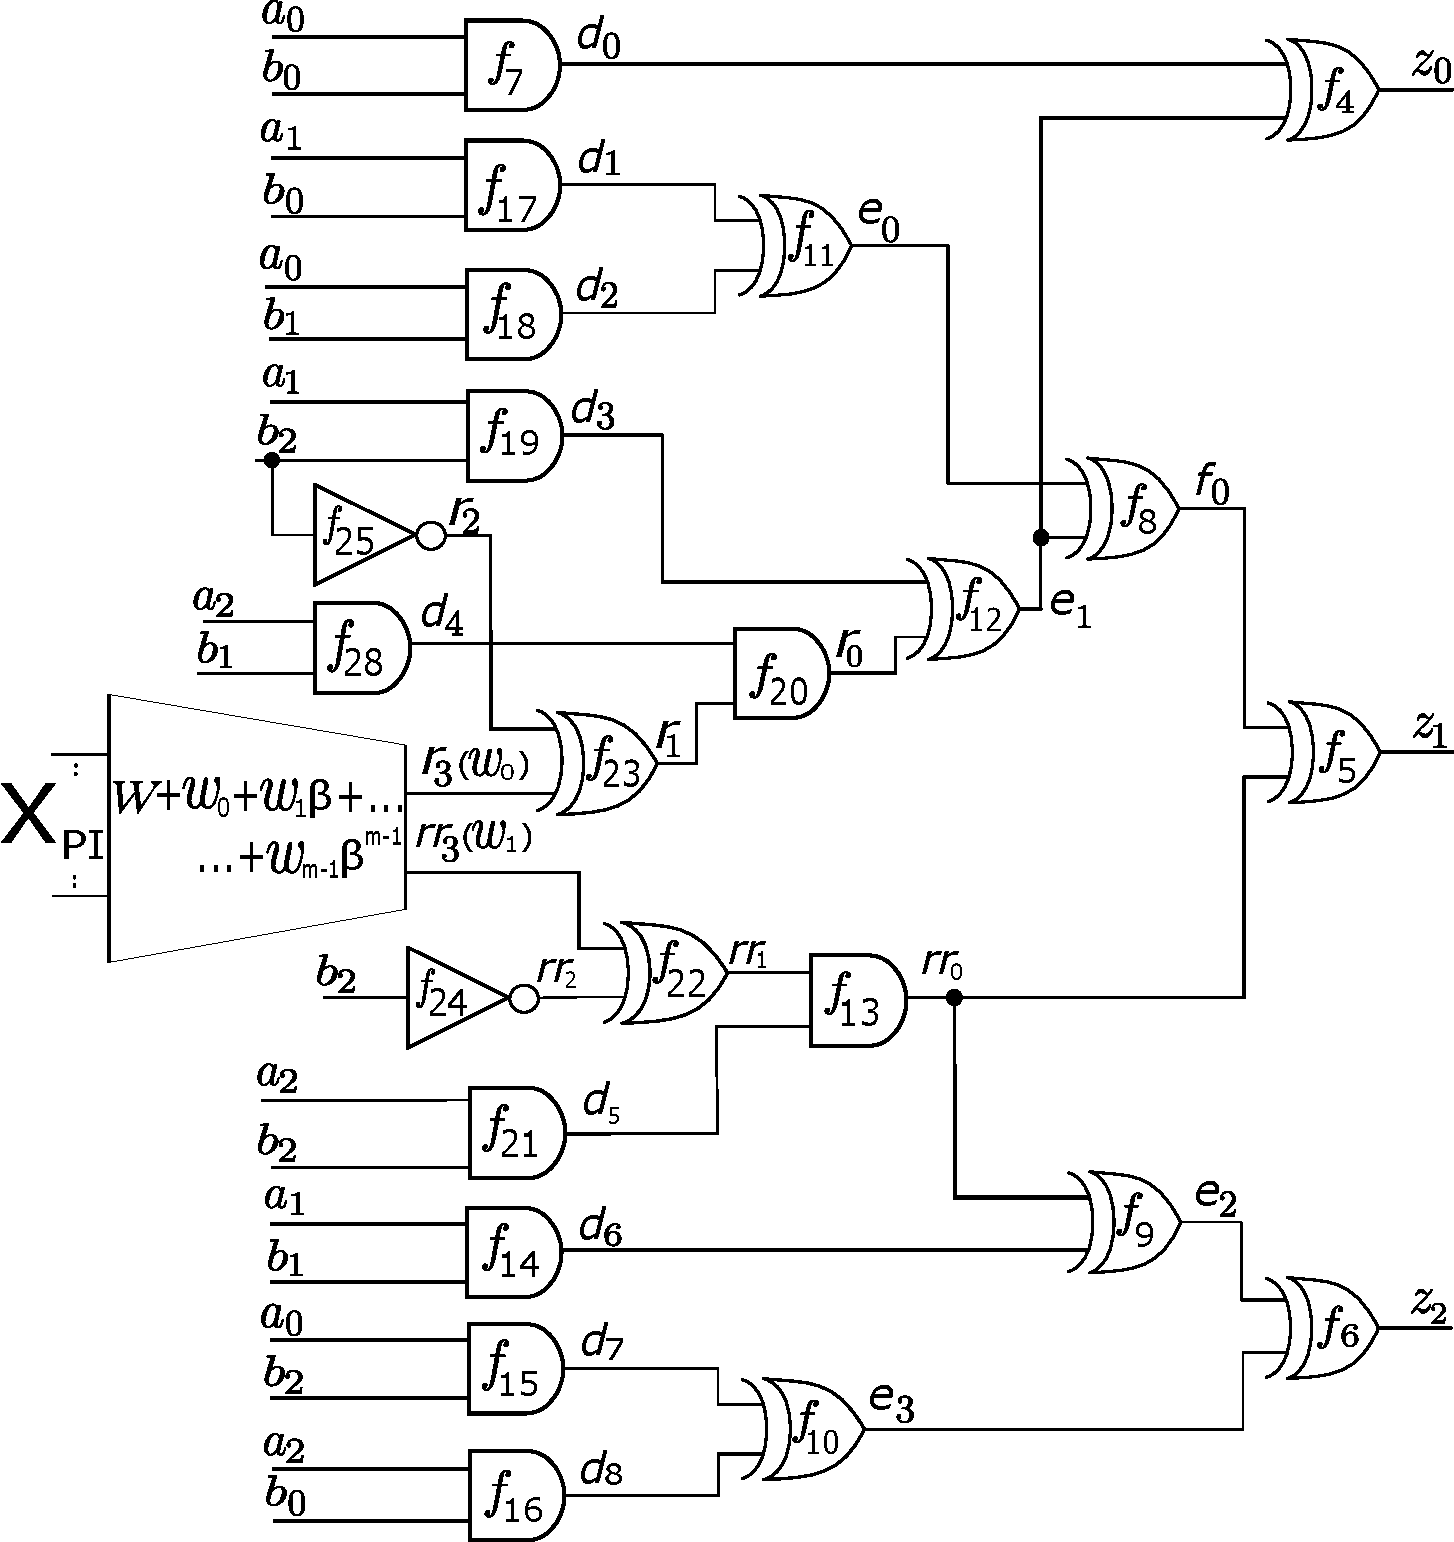
\includegraphics[scale = 0.24]{mas_3_ddc_mfr_b.pdf}
    \caption*{
    Patch function modeled as a 2-bit-vector word ($m$=2), 
    $f_W: W+ r_3 + \beta \cdot rr_3$}
\end{figure}
\end{frame}

\begin{frame}{\large Application: Computing $P_k(x)$}
\bi
\item $P_3(x) = x^3+x+1,~~P_2(x) = x^2+x+1,~~\ga = \al^9,~~\be=\alpha^{21}$
\pause
\vspace{0.1in}
	\item Composite field: $k=LCM(2,3)=6$
	\vspace{0.1in}
	\pause
	\bi
		\item $ UPF(P_3(x^9)) = (x^9)^3+(x^9)+1 =
  \textcolor{red}{(x^6+x^5+x^2+x+1)}\textcolor{green}{(x^6+x^5+1)}\textcolor{green}{(x^6+x^4+x^3+x+1)}(x^6+x^4+x^2+x+1)(x^3+x+1);$
		\vspace{0.1in}
		\pause
		\item $UPF(P_2(x^{21})) = (x^{21})^2+(x^{21})+1 =
  \textcolor{red}{(x^6+x^5+x^2+x+1)}\textcolor{green}{(x^6+x^5+1)}\textcolor{green}{(x^6+x^4+x^3+x+1)}(x^6+x^5+x^3+x^2+1)
  (x^6+x^5+x^4+x+1)(x^6+x+1)(x^6+x^3+1);$
		% \pause
		% \vspace{0.1in}
		% \item We choose $P_6(x)=x^6+x^5+1$ as the required $P_k(x)$.
	\ei
\ei
\end{frame}

% \begin{frame}{\large Circuit polynomials over $\Fkk$}
% \bi
% 	\item Boolean logic gates in $\F_2 ~~(\F_2 \subset \Fkk)$. Over $\F_2$, $-1=+1\pmod{2}$
% \ei
% 	\begin{align*}
% 		 z &=~ \sim a &\implies &z+a+1 &\pmod{2}\\
% 		 z &= a \wedge b &\implies &z+a\cdot b &\pmod{2}\\
% 		 z &= a \vee b &\implies &z+a\cdot b + a + b &\pmod{2}\\
% 		 z &= a \oplus b &\implies &z+a+b &\pmod{2}
% 	\end{align*}
% \pause
% \bi
% 	\item Word-level polynomials with $\ga = \al^{\lambda}$ and $\be = \al^{\mu}$
% 	% \bi 
% 		% \item $\ga$ = primitive element of $\Fkn$, i.e. $P_n(\ga)=0$
% 	% \ei
% \ei
% \begin{equation*}
% \begin{split}
%  Output:& Z + z_0 +\gamma \cdot  z_1 + \dots +\gamma^{n-1} \cdot z_{n-1}\\
%  Input: & A + a_0 +\gamma \cdot a_1 + \dots +\gamma^{n-1} \cdot a_{n-1} \\
%  Patch: & W + w_0 +\beta \cdot w_1 + \dots +\beta^{m-1} \cdot w_{m-1}
% \end{split}
% \end{equation*}
% \end{frame}

\begin{frame}{\large Circuit Polynomials and Setup}
\bi
	\item Ring $R = \Fkk[Z,A,B,\dots,W,r_3,rr_3,\dots,a_0,a_1,\dots,b_1,b_2]$ 
	\vspace{0.1in}
	\pause
	\item Circuit polynomials under a term order $>$:
	\begin{small}
	\begin{flalign*}
	f_1:Z + z_0 +\ga \cdot z_1 + \ga^2 \cdot z_2;   &\quad f_{22}:rr_1 + rr_3+rr_2; \\
	f_2:A + a_0 +\ga \cdot a_1 + \ga^2 \cdot a_2;   &\quad f_{23}:r_1 + r_2+r_3;\\
	f_3:B + b_0 +\ga \cdot b_1 + \ga^2 \cdot b_2;   &\quad \red{f_{26}:r_3 + r_4 + d_4;}\\
	f_4:z_0 + d_0 + e_1;                &\quad {\red f_{27}:rr_3 + rr_4 + b_2;}\\
	f_5:z_1 + f_0 + rr_0;               &\quad \dots\\
	\dots                               &\quad f_{30}:rr_4 + a_2+b_2+a_2b_2; \\
	\dots								&\quad f_W:W + r_3 + \be \cdot rr_3;
	\end{flalign*}
	\end{small}
	\vspace{-0.2in}
	\pause
	\item $F = \{f_1,\dots,f_{30},f_W\}$
	\item $F_0 =\{a_0^2-a_0,\dots,z_2^2-z_2,A^8-A,\dots,Z^8-Z,W^4-W\}$. 
	% \bi
	% 	\item Ideal $J+J_0=\langle F\cup F_0\rangle$ models $C$.
	% \ei
\ei

\end{frame}
% \begin{frame}{\large MFR Notation: Incorrect $P_k(x)$}
% \bi
% 	\item If we incorrectly choose $P_k(x)=x^6+x^3+1$
% 	\pause
% 	\item For its root $\al$, we have
% 	\pause
% 	\begin{align*}
% 	\alpha^6 + \alpha^3 + 1 &= 0\\
%  	(\alpha^3)(\alpha^6 +\alpha^3 + 1) &= 0 ~(\text{multiply by}~\alpha^3)\\
% 	\alpha^9 + \alpha^6 + \alpha^3 &= 0 \\
% 	\gamma + 1 &= 0
% % \stepcounter{equation}\tag{\theequation}\label{ll} 
% \end{align*}
% 	\pause
% 	\item However, $\ga \neq 1$, as $\ga$ is a primitive element of $\Fkn$
% 	\item Selecting arbitrary $P_k(x)$ leads to erroneous results
% \ei
% \end{frame}

% \begin{frame}{\large Application: Word-level representation}
% \begin{figure}[hbt]
% \centering
%     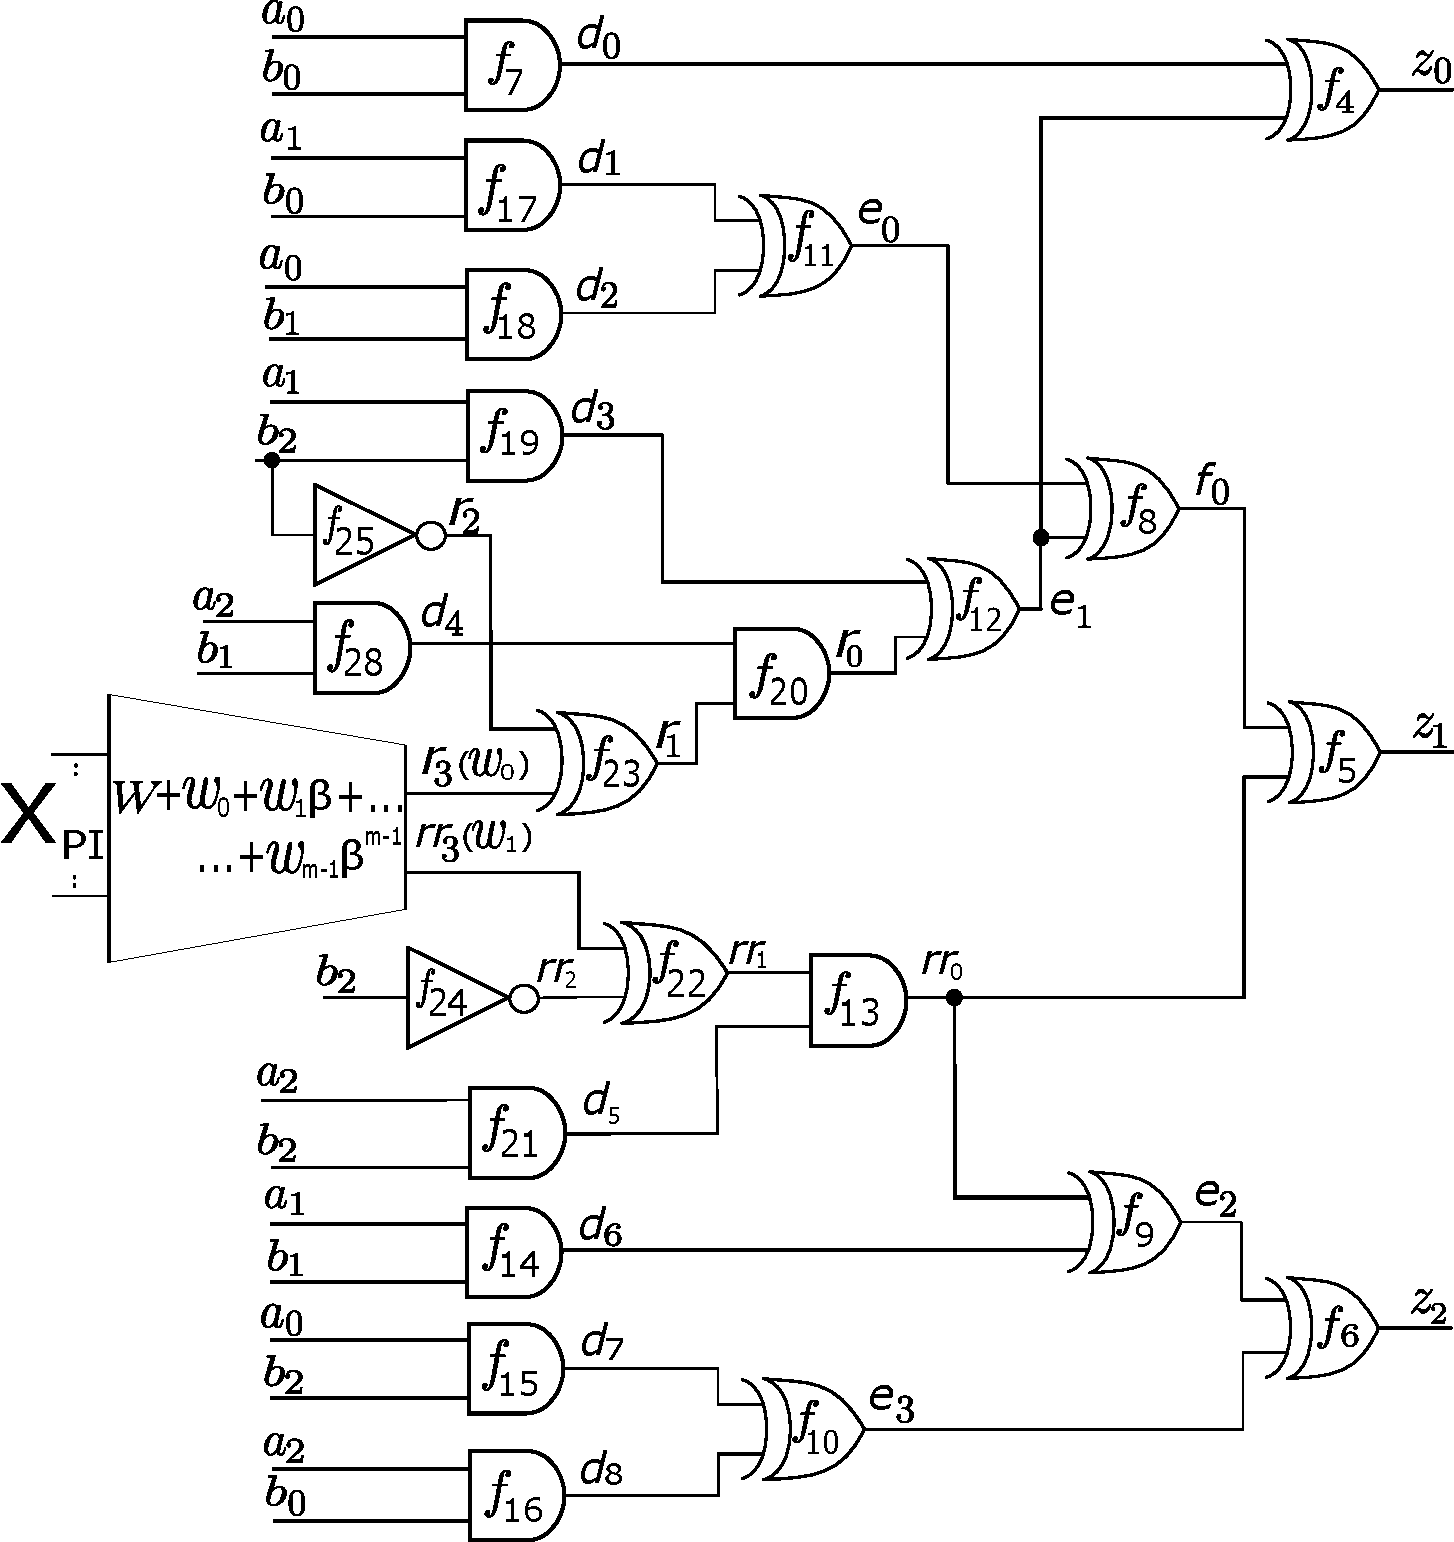
\includegraphics[scale = 0.24]{mas_3_ddc_mfr_b.pdf}
%     \caption*{
%     Patch function modeled as a 2-bit-vector word ($m$=2), 
%     $f_W: W+ r_3 + \beta \cdot rr_3$}
% \end{figure}
% \end{frame}


% \begin{frame}{\large MFR Notation: Word-level reasoning}
% \bi
% 	\item Obtain each $w_i$ as a polynomial function in $W,\beta$
% 	\bi
% 		\item $\forall i \in 1,\dots,m,~~w_i= \mathcal{F}_i(W,\beta)$
% 	\ei
% 	\pause
% 	\begin{align*}
% 	W & = w_0 + \dots + \beta^{m-1} \cdot w_{m-1}\\
%     W^2 & = w_0^2 + \dots + \beta^{2(m-1)}\cdot w_{m-1}^2\\
%         & \dots \\
%     W^{2^{m-1}} & = w_0 + \dots + \beta^{2^{m-1}(m-1)}\cdot w_{m-1}
%     \end{align*}
% 	\pause
% 	\item Solved using Gaussian elimination
% \ei
% \end{frame}

% \begin{frame}{\large MFR Notation: MFR setup steps}
% \begin{enumerate}
% 	\item Setup a new ring $R' = \Fkk[x_1,\dots,x_d,Z,A,W]$ 
% 	\bi
% 		\item $\Fkk$ is constructed using $P_k(x)$
% 		\item Modify RTTO $>$ to place the target $W$ before the lowest indexed target $w_i$
% 	\ei
% 	\vspace{0.1in}
% 	\pause
% 	\item Construct a polynomial set $F'$ as follows:
% 	\bi
% 		\pause
% 		\item Start with $F' = F$
% 		\pause
% 		\item Remove polynomials with $w_i$'s as leading terms
% 		\pause
% 		\item Substitute $\forall i \in 1,\dots,m,~~w_i= \mathcal{F}_i(W,\beta)$
% 		\pause
% 		\item Add $f_w: W + \sum_{i=0}^{m-1}\be^iw_i$
% 		\pause
% 		\item Substitute $\beta = \alpha^{\mu}, \gamma=\alpha^{\lambda}$
% 	\ei

% \end{enumerate}
% \end{frame}


% \begin{frame}{\large Circuit Polynomials and Setup}
% \bi
% 	\item Ring $R = \Fkn[x_1,\dots,x_d,Z,A]$ 
% 	\bi
% 		\item $\Fkn$ is constructed using $P_n(x)$
% 	\ei
% 	\item Circuit polynomials under RTTO $>$:
% 	\begin{small}
% 	\begin{flalign*}
% 	f_1:Z + z_0 +\ga \cdot z_1 + \ga^2 \cdot z_2;   &\quad f_{22}:rr_1 + rr_3+rr_2; \\
% 	f_2:A + a_0 +\ga \cdot a_1 + \ga^2 \cdot a_2;   &\quad f_{23}:r_1 + r_2+r_3;\\
% 	f_3:B + b_0 +\ga \cdot b_1 + \ga^2 \cdot b_2;   &\quad \red{f_{26}:r_3 + r_4 + d_4;}\\
% 	f_4:z_0 + d_0 + e_1;                &\quad {\red f_{27}:rr_3 + rr_4 + b_2;}\\
% 	f_5:z_1 + f_0 + rr_0;               &\quad \dots\\
% 	\dots                               &\quad f_{30}:rr_4 + a_2+b_2+a_2b_2;
% 	\end{flalign*}
% 	\end{small}
% 	\vspace{-0.1in}
% 	\item $F = \{f_1,\dots,f_{30}\}$, $F_0 =\{a_0^2-a_0,\dots,z_2^2-z_2,A^8-A,\dots,Z^8-Z\}$. 
% 	\bi
% 		\item Ideal $J+J_0=\langle F\cup F_0\rangle$ models $C$.
% 	\ei
% \ei

% \end{frame}

% \begin{frame}{\large MFR Application: Word-level Formulation }
% \bi
% 	\item ring $R' = \F_{2^6}[x_1,\dots,x_d,Z,A,W]$ 
% 	\bi
% 		\item $\F_{2^6} = \F_2[x]$ (mod $P_6(x)$), $P_6(x) = x^6+x^5+1$
% 		\pause 
% 		\vspace{0.1in}
% 		\item WRTO $>$: {\small 
% $\{Z\}>\{A>B\}>\{z_0>z_1>z_2\}>\cdots>\{d_1>d_2>d_3>r_0>d_5>rr_1\}>
% \{r_1\}>{\bf \{W\}}>\{{\bf rr_3}>rr_2\}>\{r_2>{\bf r_3}>rr_4\}>\{r_4>d_4\}>\{a_0>a_1>a_2>b_0>b_1>b_2\}$}

% 	\ei
% 	\vspace{0.1in}
% 	\pause
% 	\item Update polynomial set $F$ to $F'$ as:
% 	\begin{align*}
% 		&rr_3= W^2+W,~~r_3 = \be W^2 +\be^2W \\
% 		&f'_{22}:rr_1  + (W^2+W) + rr_2\\
% 		&f'_{23}:r_1 + r_2 + (\be W^2 +\be^2 W)\\
% 		&f_W:W + r_3 + \be \cdot rr_3\\     
% 		&\be=\al^{21} \text{ and } \ga=\al^9 \\
% 		&F'=\{f_1,\dots,f_{21},~f'_{22},f'_{23},f_W,\dots,f_{30}\}-\{f_{26},f_{27}\}
% 	\end{align*}
% \ei
% \end{frame}

% \begin{frame}{\large MFR Contribution: Rectification Check}
% %ATPG V() V() = empty
% %we have an algebraic proof which is there in the proposal
% \bi
% 	\item Multi-fix rectification at target $W$
% 	\vspace{0.1in}
% 	\bi
% 		\item Construct the following polynomial sets:
% 		\begin{align*}
% 			F_l' =\langle f_1,\dots,f_W=W+\delta[l],\dots,f_s\rangle,1 \leq l \leq 2^m, \\
% 			% \text{ where $F_l'$ is obtained from $F'$ by replacing } \\
% 			% f_W \in F' \text{ with } f'_W: W + \delta[l], 1\leq l \leq 2^m,\text{ and } \\
%   			Where~(\delta[1],\dots,\delta[2^{m}]) =(0,1,\be,\dots,\be^{2^m-2}).
% 		\end{align*}
% 		\pause
% 		\item Reduce the specification $f: Z+A\cdot B$ modulo these sets: 
% 		\bi
% 			\item $f\xrightarrow{F_l', F_0}_+rem_l $, $\forall 1 \leq l \leq 2^m$
% 		\ei
% 		% \item Let $V_{\Fq}(rem_l)$ denote the varieties of the respective $rem_l$'s
% 		\vspace{0.2in}
% 		\pause
% 		\item Multi-fix rectification exists at target $W$: \\  
% 				\centering
% 				{\bf if and only if} $ \prod_{l=1}^{2^m} rem_l \xrightarrow{F_0}_+0$
% 	\ei
% \ei
% \end{frame}

\begin{frame}{\large Rectification check: Remainder generation}
\begin{figure}[hbt]
\centering
    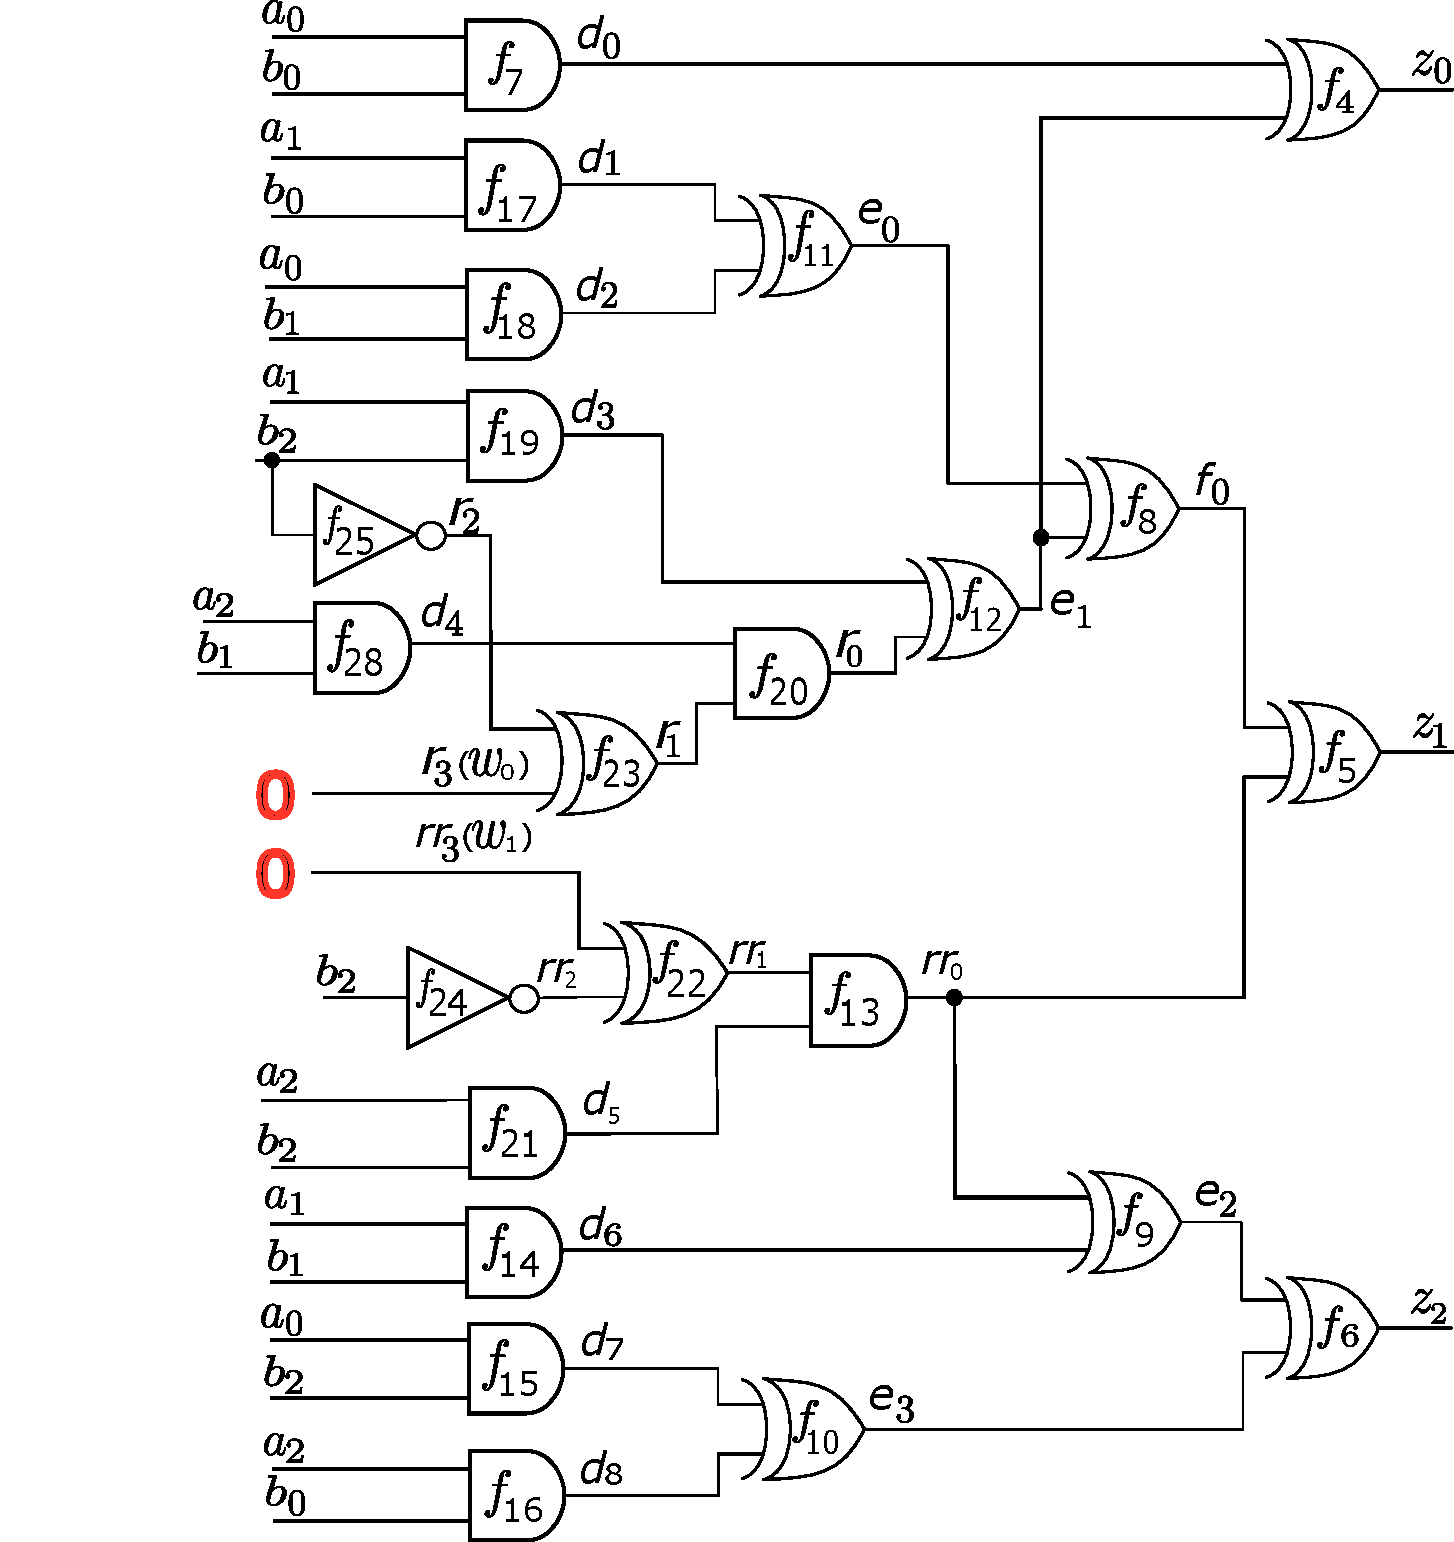
\includegraphics[scale = 0.28]{mas_3_ddc_mfr_b_00.pdf}
    \caption*{}
\end{figure}
\end{frame}

\begin{frame}{\large Rectification check: Remainder generation}
\begin{figure}[hbt]
\centering
    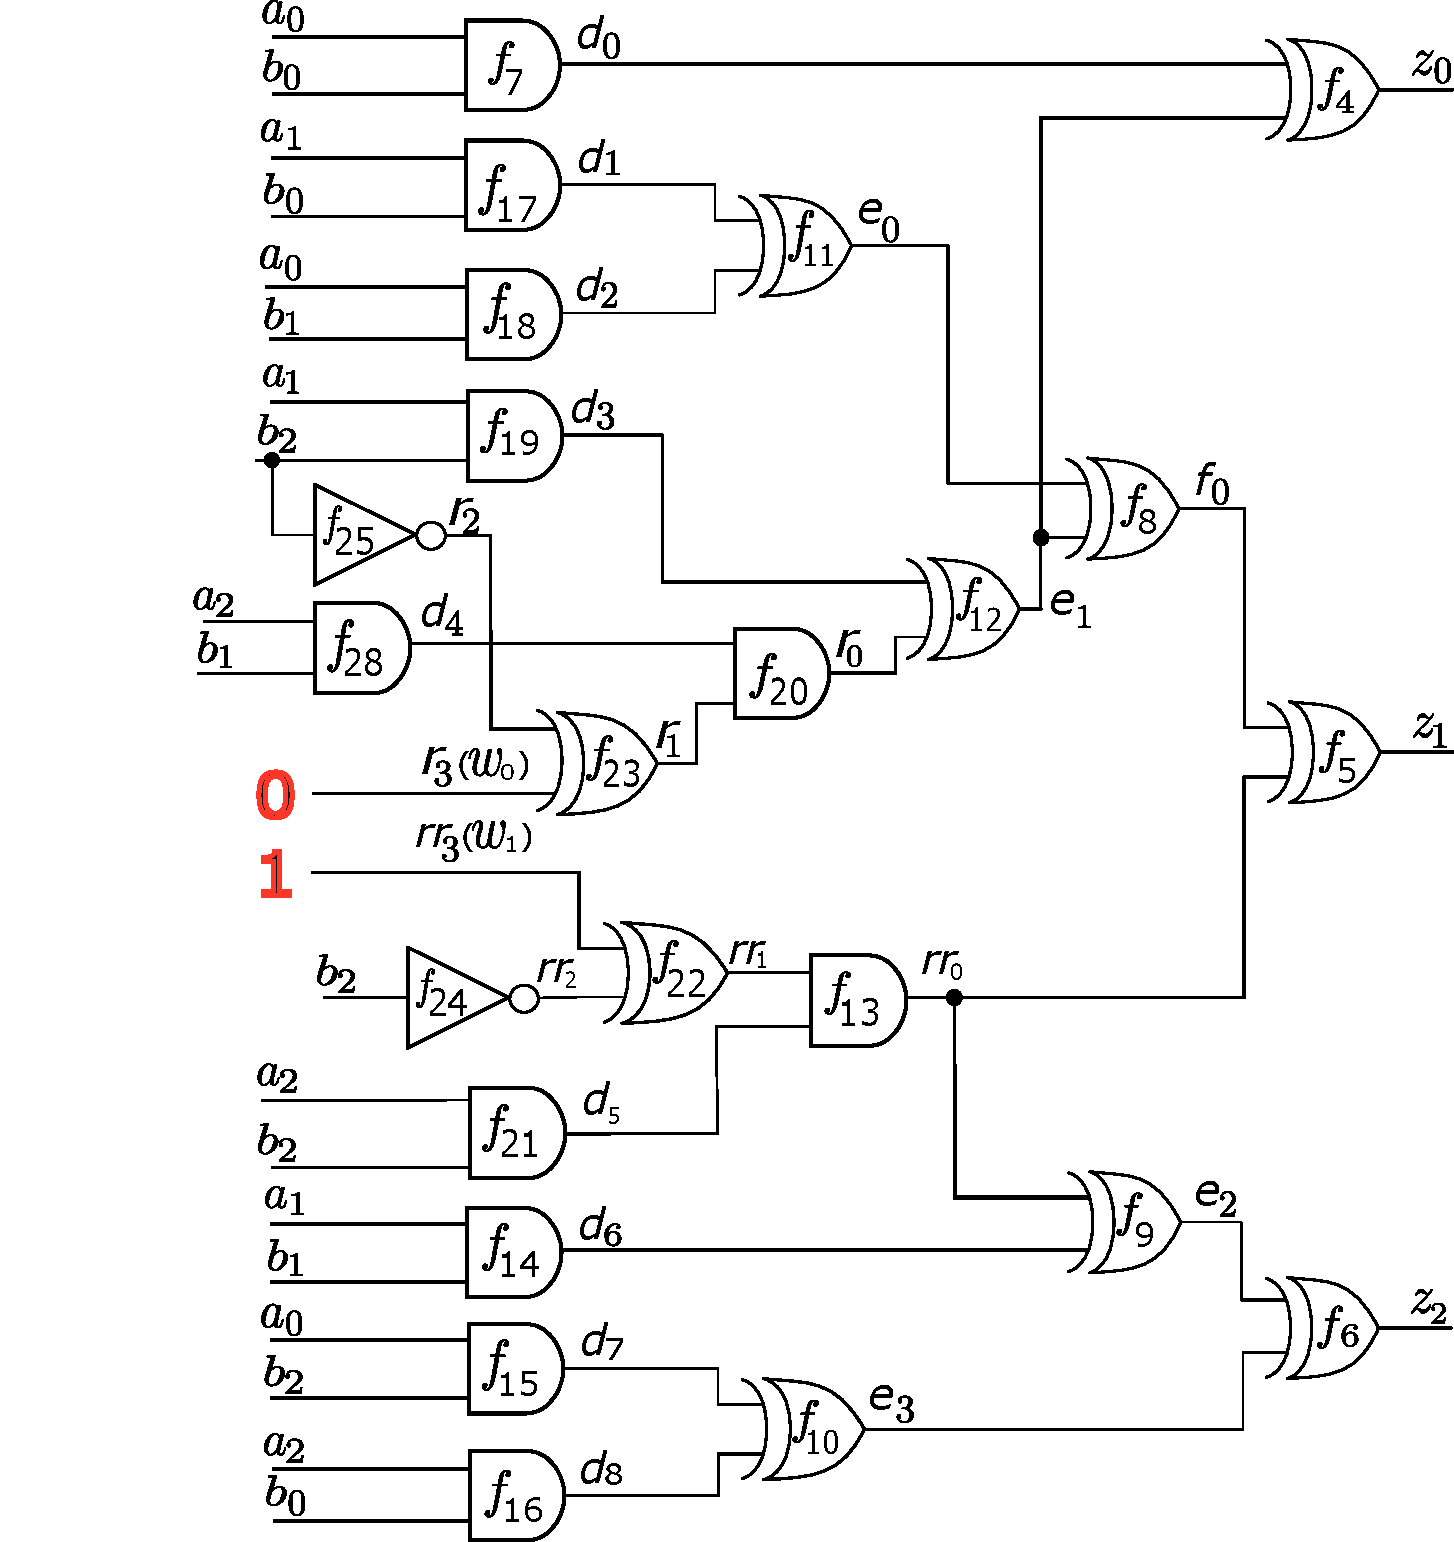
\includegraphics[scale = 0.28]{mas_3_ddc_mfr_b_10.pdf}
    \caption*{}
\end{figure}
\end{frame}

\begin{frame}{\large Rectification check: Remainder generation}
\begin{figure}[hbt]
\centering
    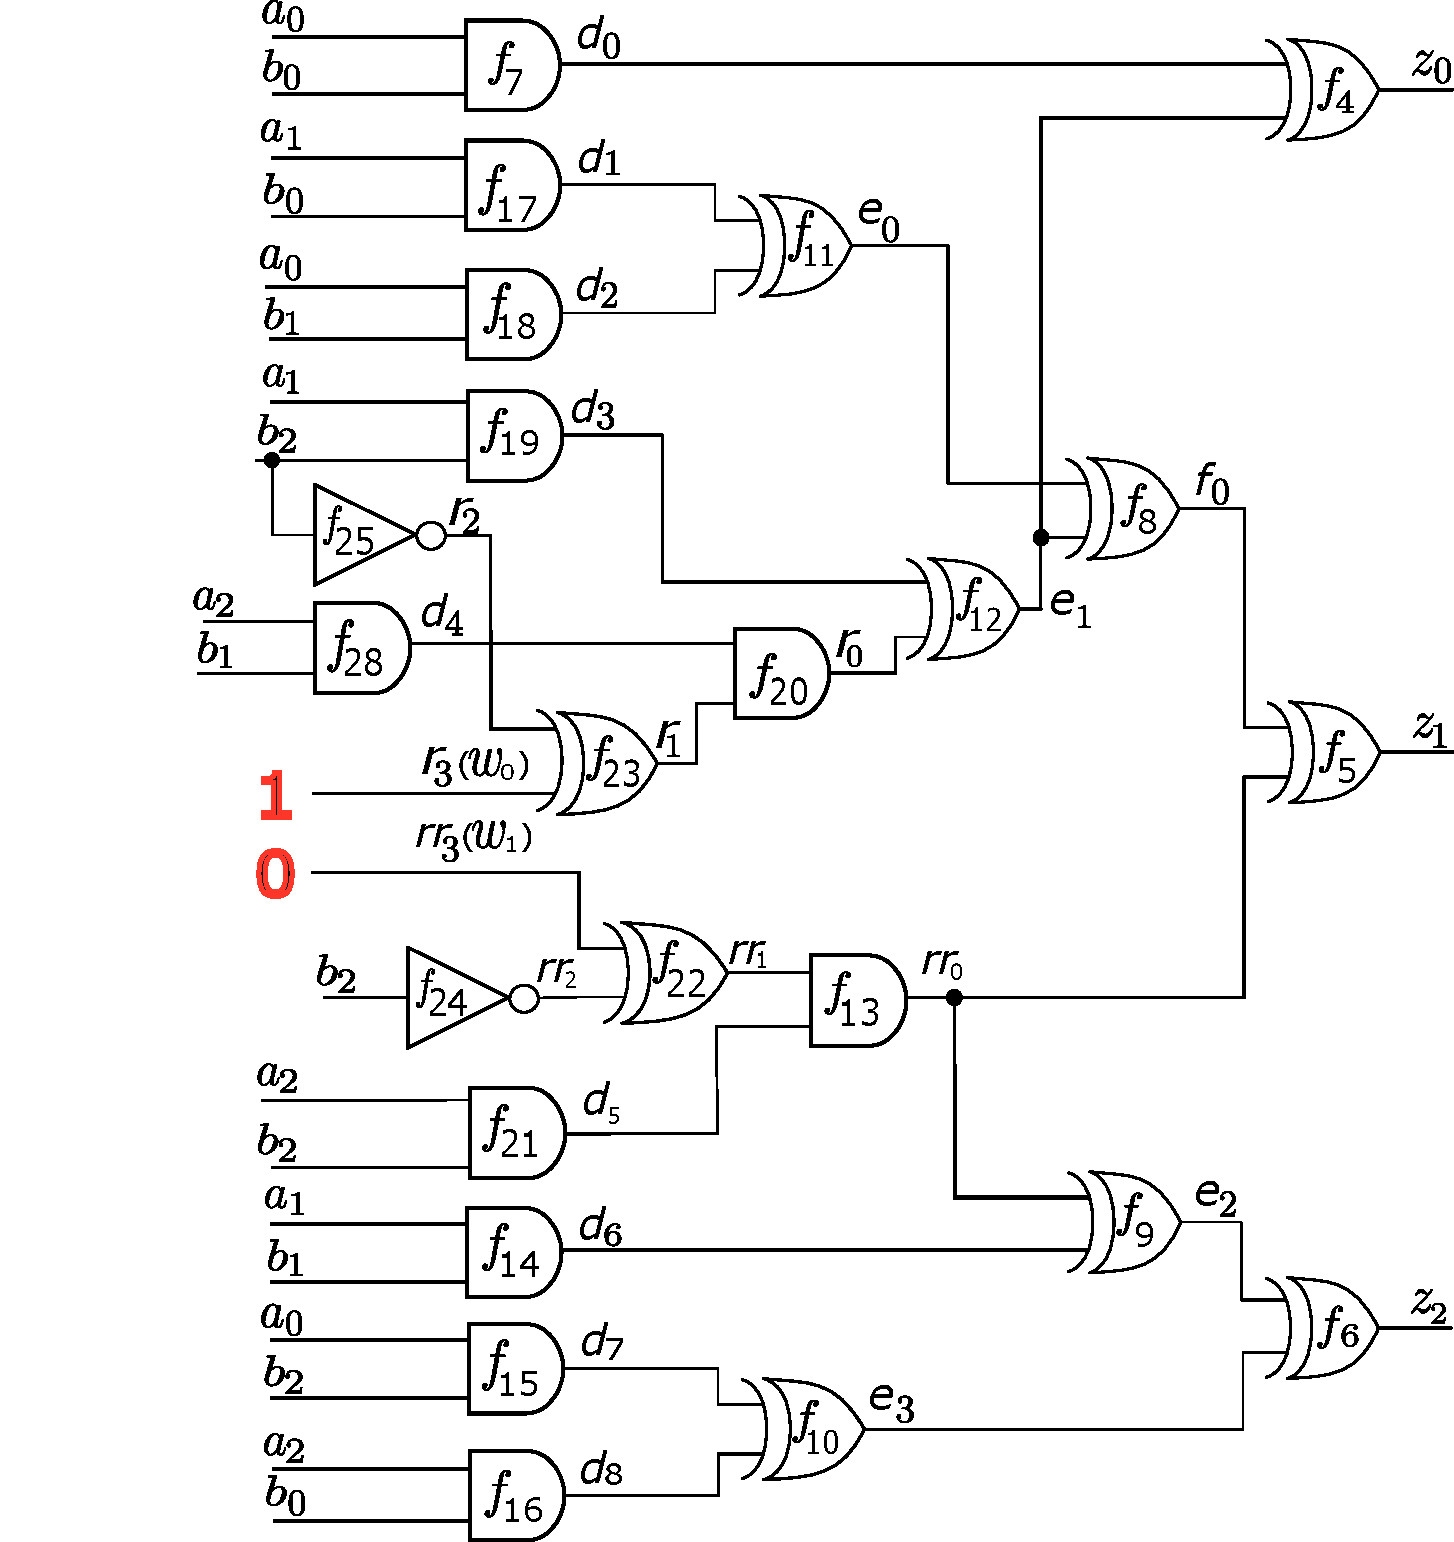
\includegraphics[scale = 0.28]{mas_3_ddc_mfr_b_01.pdf}
    \caption*{}
\end{figure}
\end{frame}

\begin{frame}{\large Rectification check: Remainder generation}
\begin{figure}[hbt]
\centering
    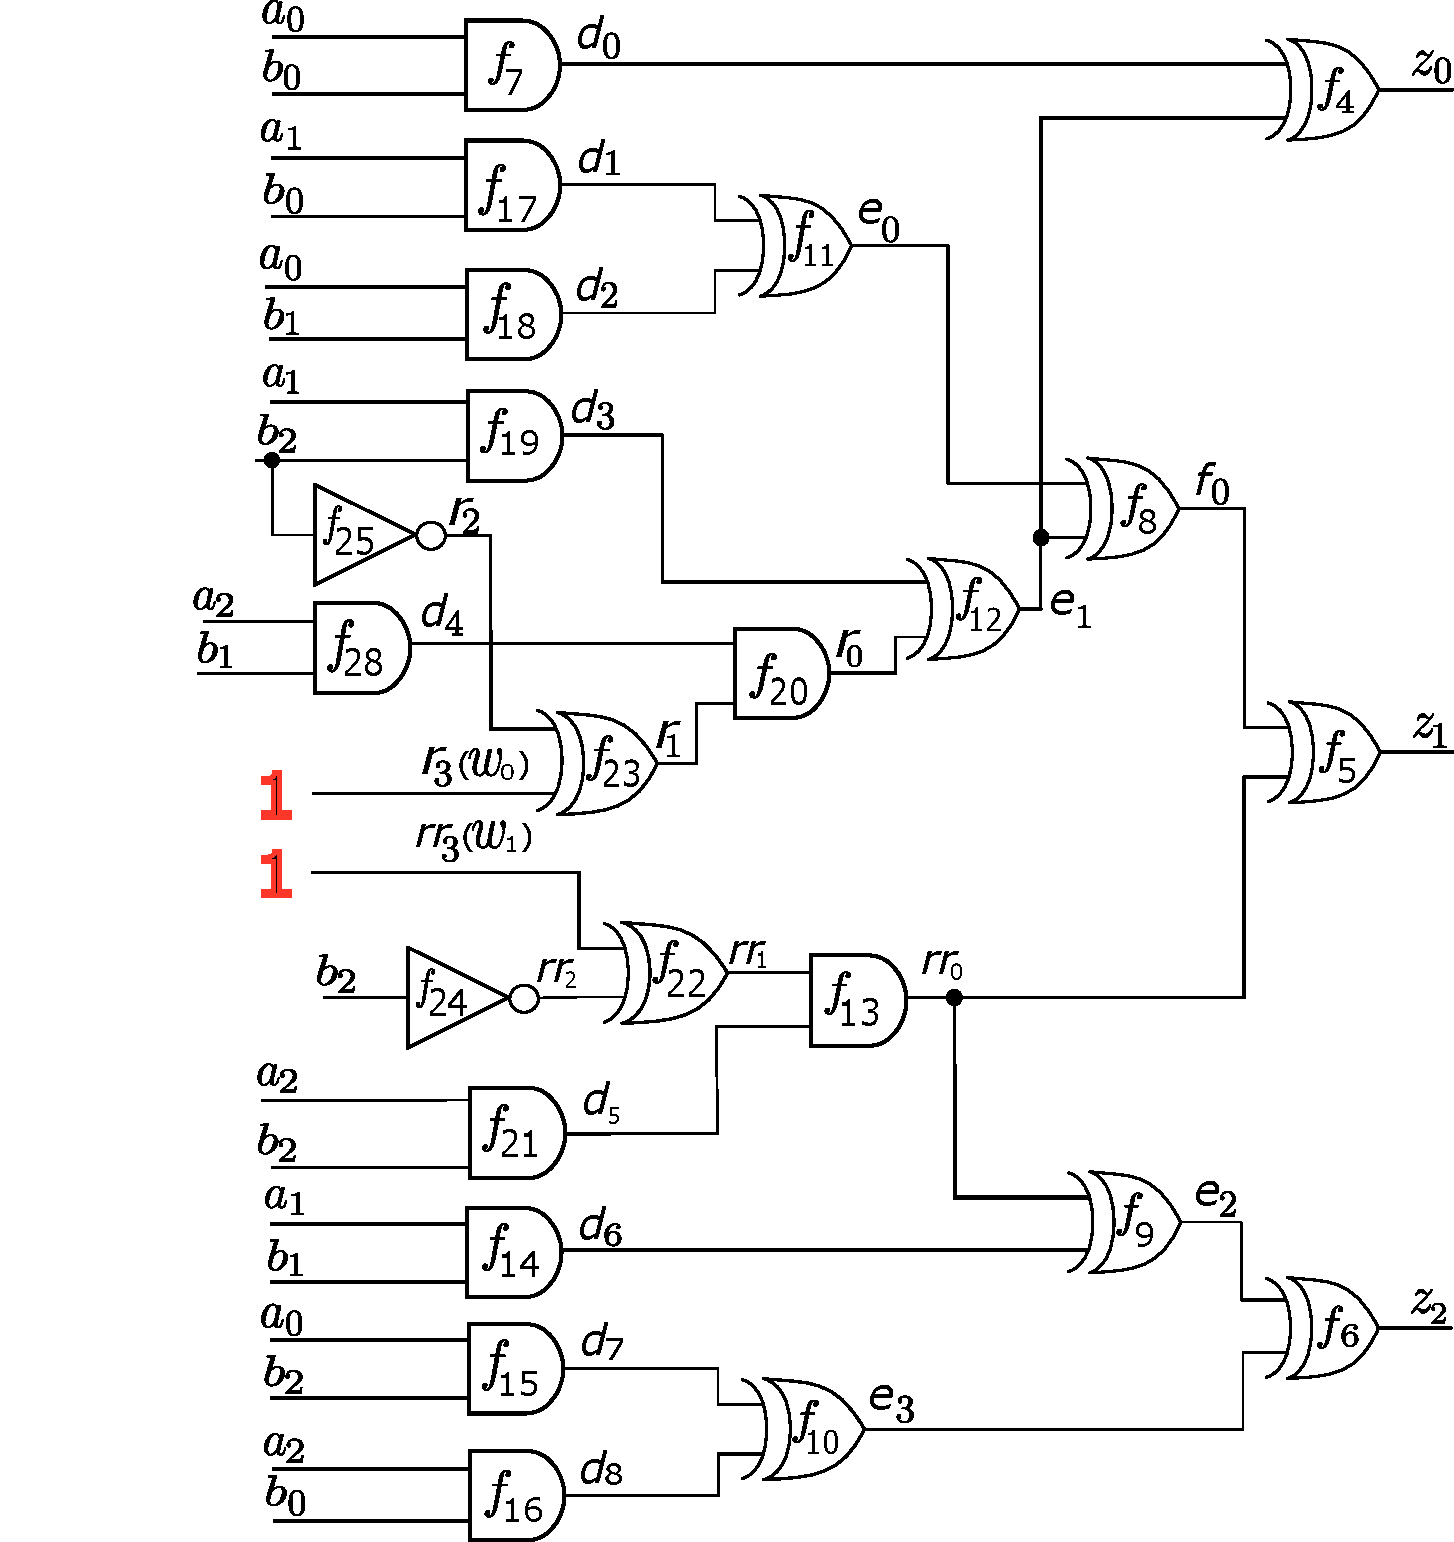
\includegraphics[scale = 0.28]{mas_3_ddc_mfr_b_11.pdf}
    \caption*{}
\end{figure}
\end{frame}

\begin{frame}{\large Contribution: Multi-fix Rectification Check}
\bi
	\item Constructing the $F'_l$:
	\bi
		\item {$F_1'$, where $F_1'[f_W]=W+\delta(1)=W$},
		\item {$F_2'$, where $F_2'[f_W]=W+\delta(2)=W+1$},
		\item {$F_3'$, where $F_3'[f_W]=W+\delta(3)=W+\be$},
		\item {$F_4'$, where $F_4'[f_W]=W+\delta(4)=W+\be^2$}
	\ei
	\vspace{0.1in}
	\pause
	\item Reducing the specification $f: Z+A\cdot B$:
\bi
\item $rem_1 = f \xrightarrow[]{F_1'\cup F_{0}}_+{\al^{27} (a_2b_1b_2)+\al^{36} (a_2b_2)}$
\item $rem_2 = f \xrightarrow[]{F_2'\cup F_{0}}_+{\al^{27} (a_2b_1b_2+a_2b_1)+\al^{36} (a_2b_2)}$
\item $rem_3 = f \xrightarrow[]{F_3'\cup F_{0}}_+{\al^{27} (a_2b_1b_2)}$
\item $rem_4 = f \xrightarrow[]{F_4'\cup F_{0}}_+{\al^{27} (a_2b_1b_2+a_2b_1)}$
\ei \pause
	\item $rem_1\cdot rem_2 \cdot rem_3 \cdot rem_4 \xrightarrow{F_0}_+0$
	\item Target $W$ with nets $r_3$ and $rr_3$ admits MFR
\ei
\end{frame}

% \begin{frame}{\large Future work: Rectification function}

% \bi
% \item A polynomial which can be computed to rectify the circuit
% 	\bi
% 		\item $W = a_2b_1b_2 + \beta \cdot a_2b_2$
% 		\item $r_3 = (a_2 \wedge b_1 \wedge b_2),~~rr_3 = (a_2 \wedge b_2)$
% 	\ei
% \ei

% \end{frame}

% \begin{frame}{\large MFR Pseudocode}
% \begin{figure}[hbt]
% \centering
%     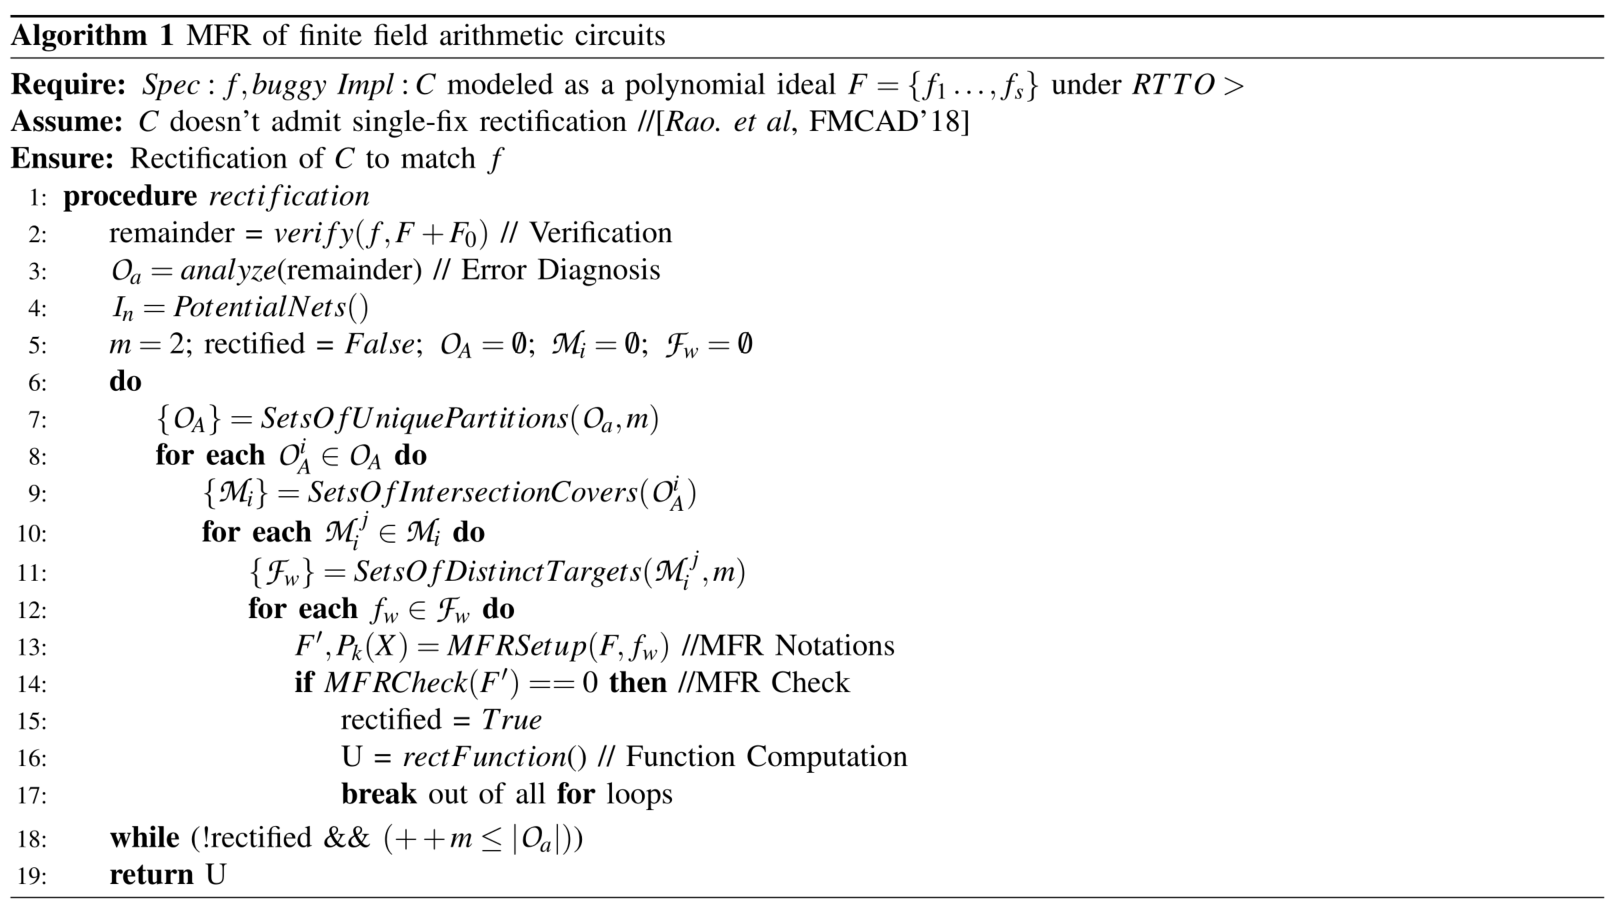
\includegraphics[scale = 0.43]{algo.png}
% \end{figure}
% \end{frame}

% \begin{frame}{\large Research Objective: Synthesis of Rectification Function}
% \begin{figure}[hbt]
%     \begin{center}
%     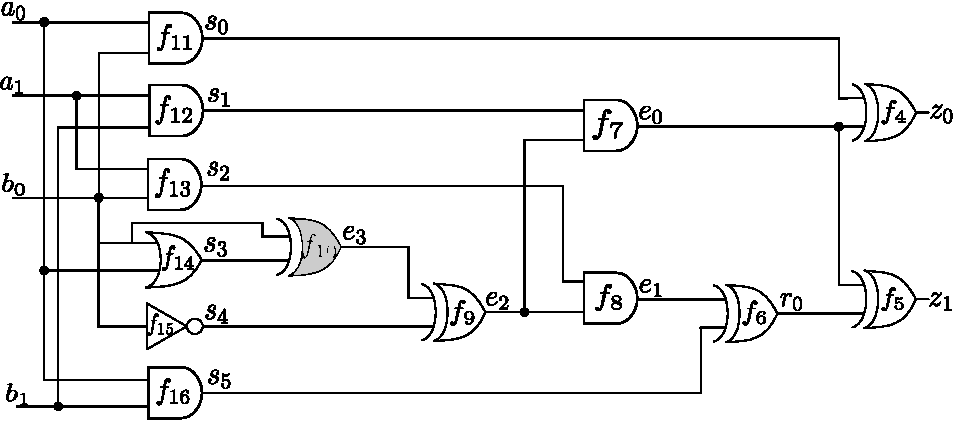
\includegraphics[scale = 0.7]{mas_red_bug-eps-converted-to.pdf}
%     \end{center}
% %    \vspace{-4ex}
%     \caption*{\small A 2-bit buggy modulo
%       multiplier implementation. 
%     %   with the bug at
%     % net $e_3$. A correct implementation will have an AND gate at $e_3$,
%     % which has been replaced by an XOR gate.
%     }
%     \label{fig:mas_both}
% \end{figure}
% \end{frame}

% \begin{frame}{\large Research Objective: Exploring don't cares}
% \begin{small}
% $r \in \langle h_{10},f_{11},f_{12},f_{13},f_{14},f_{15},f_{16}\rangle
%   + \langle F_{0}^{PI}\rangle$ \\
% $r = U\cdot h_{10} + h_{11}f_{11} + h_{12}f_{12}+h_{13}f_{13}+h_{14}f_{14}+h_{15}f_{15}+h_{16}f_{16}$ \\
% $U = b_0$; $U^1 = a_1*b_0$; $U^2 = a_1*b_1*b_0+a_1*b_1+a_1$;
% \end{small}
% {\tiny 
% \begin{table}[ht]
%     \centering
%     \begin{tabular}{|c|c|c|c|c|} \hline
%       $\{a_0a_1b_0b_1\}$ & $h_{10}$ & $U$ & ${U^1}$ & ${U^2}$ \\ \hline
% 		0000 & 0     & 0 & 0 & 0 \\ \hline
% 		0001 & 0     & 0 & 0 & 0 \\ \hline
% 		0010 & 0     & 1 & 0 & 0 \\ \hline
% 		0011 & 0     & 1 & 0 & 0 \\ \hline
% 		0100 & 0     & 0 & 0 & 1 \\ \hline
% {\it    0101}& (x+1) & 0 & 0 & 0 \\ \hline
% {\bf    0110}& (x)   & 1 & 1 & 1 \\ \hline
% {\bf	0111}& 1     & 1 & 1 & 1 \\ \hline
% 		1000 & 0     & 0 & 0 & 0 \\ \hline
% 		1001 & 0     & 0 & 0 & 0 \\ \hline
% 		1010 & 0     & 1 & 0 & 0 \\ \hline
% 		1011 & 0     & 1 & 0 & 0 \\ \hline
% 		1100 & 0     & 0 & 0 & 1 \\ \hline
% {\it    1101}& (x+1) & 0 & 0 & 0 \\ \hline
% {\bf    1110}& (x)   & 1 & 1 & 1 \\ \hline
% {\bf    1111}& 1     & 1 & 1 & 1 \\ \hline
%     \end{tabular}
%     \caption{Evaluating quotient and rectification solutions}
% \end{table}}

% \bi
% 	\item Challenge: Word-level formulation of don't cares
% \ei

% \end{frame}

% \begin{frame}{\large Research Objective: Logic optimization using don't cares}
% \bi
% 	\item $h_{10}$ represents the ODCs for the selected target $e_3$
% 	\bi
% 		\item Algorithm to explore don't care setup
% 	\ei
% 	\vspace{0.1in}
% 	\item Logic simplification using permissible functions
% 	\bi
% 		\item {\it Fujita} has an approach using BDDs
% 		\item Investigate the application in algebraic setting
% 	\ei
% \ei
% \end{frame}


% \begin{frame}{\large Research Objective: Rectification with Min. Topological Changes}
% \begin{figure}
% \centering
% 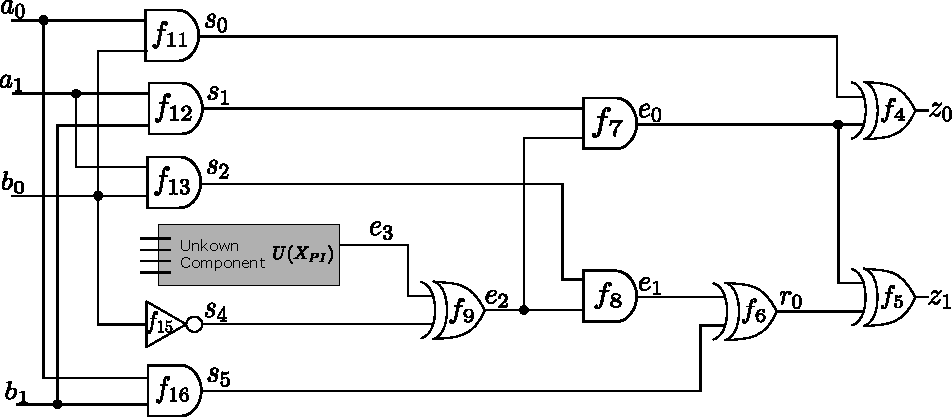
\includegraphics[scale=0.5]{mas_redundant_U.pdf}
% \end{figure}
% \bi
% 	\item In current formulation $U$ function of $X_{PI}$
% 	\item Disadvantage if net closer to PO
% 	\bi
% 		\item Re-synthesize significant portion of circuit
% 	\ei
% \ei
% \end{frame}

% \begin{frame}{\large Research Objective: Rectification with Min. Topological Changes}
% \begin{figure}
% \centering
% 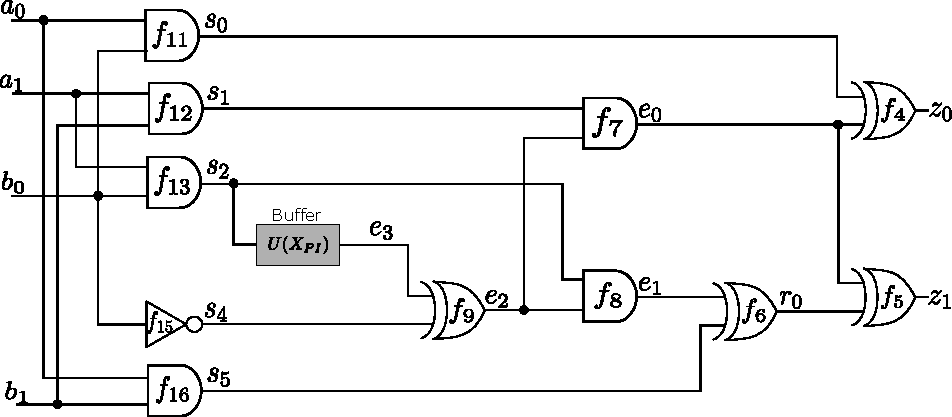
\includegraphics[scale=0.5]{mas_redundant_U_rewire.pdf}
% \end{figure}
% \bi
% 	\item Objective: Obtain $U$ in internal variables
% 	\bi
% 		\item Reuse already implemented logic
% 		\item Minimum (minimal) changes to the existing circuit
% 	\ei
% 	\item Approach: Different term orders for rectification formulation
% 	\bi
% 		\item Expensive GB computations in reduction procedures as RTTO $>$ is modified
% 	\ei
% \ei
% \end{frame}


% \begin{frame}{\large Research Objective: Integer arithmetic circuits}
% \begin{figure}[H]
%     \centering
%     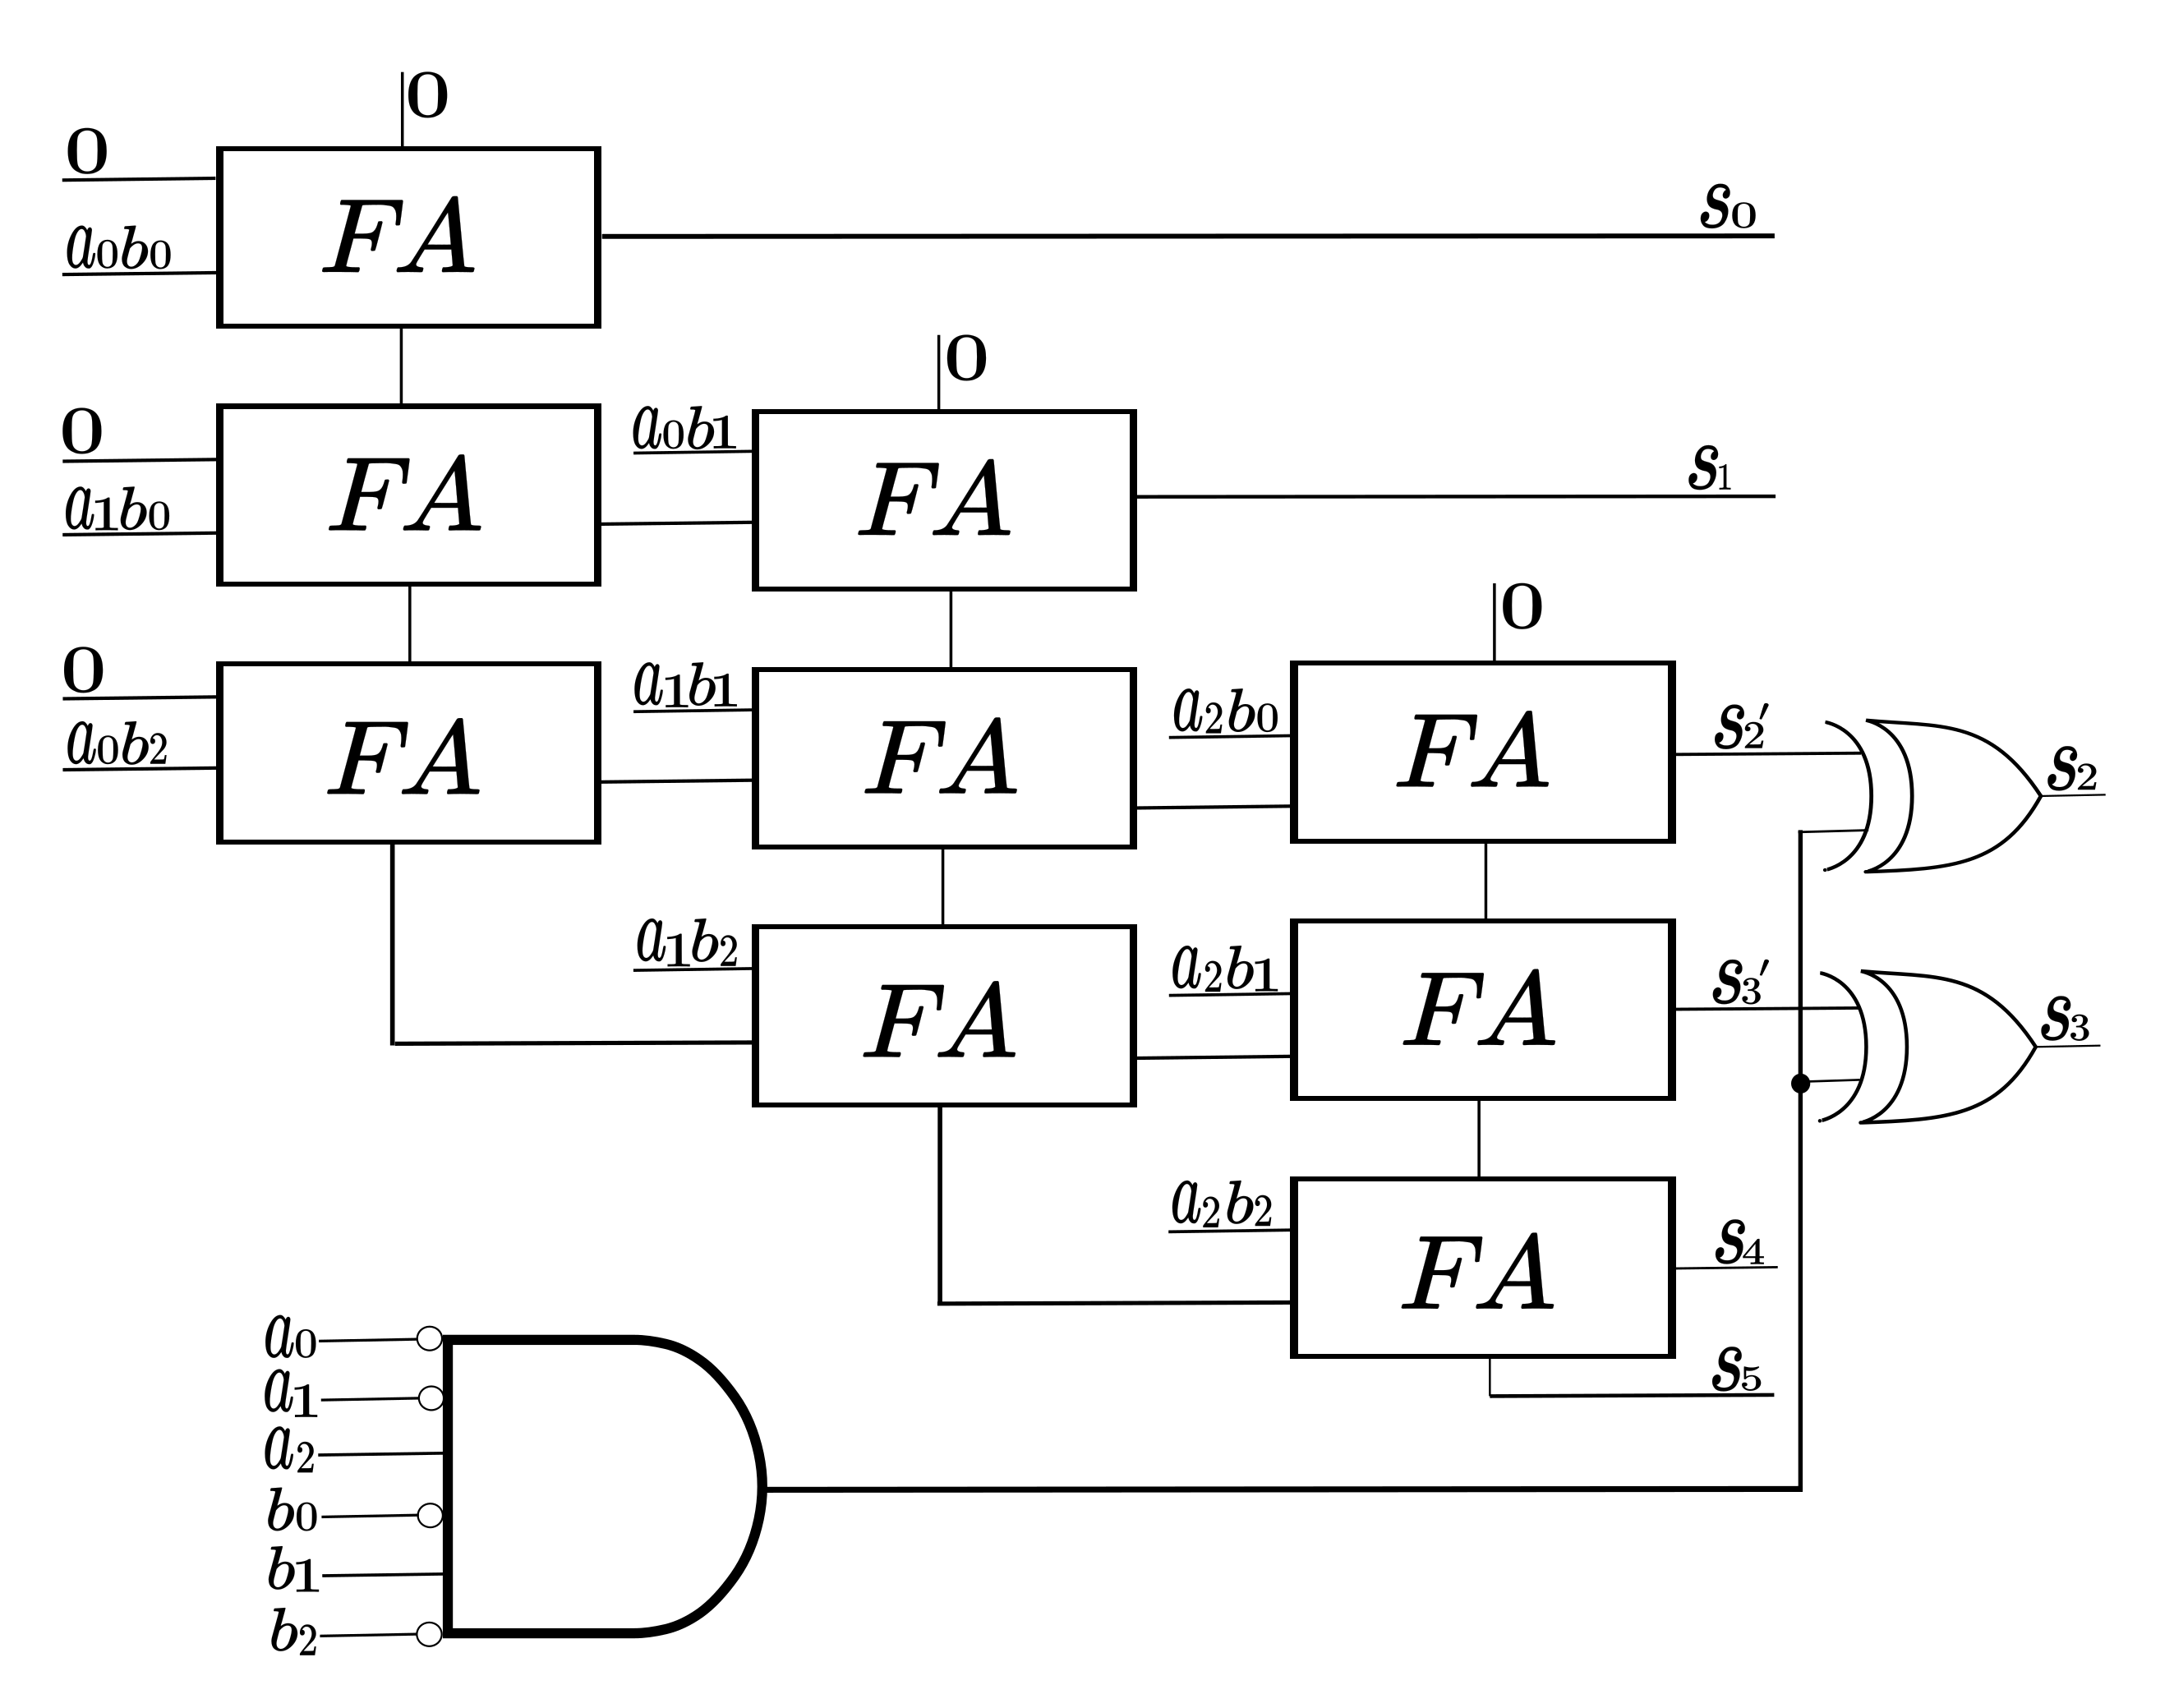
\includegraphics[scale = 0.07]{3appmult.png}
%     \caption{3-bit multiplier with additional circuit to introduce a bug}
%     \label{fig:3appmult}
% \end{figure}

% \end{frame}

% \begin{frame}{\large Research Objective: Integer arithmetic circuits}
% \bi
% 	\item Techniques valid over fields are inapplicable over rings
% 	\item \Grobner basis and division algorithms are complicated
% 	\item Can be modeled over $\Q$
% 	\bi
% 		\item Rectification function computation can result in {\it fractional coefficients}
% 		\item Extracting Boolean rectification function requires exhaustive simulation
% 		\item No scope of optimization as Extended \Grobner basis technique gives zero control
% 	\ei
% \ei

% \end{frame}

% \begin{frame}{\large Research Objective: Integer arithmetic circuits}


% {\tiny
% \begin{equation}
%     \begin{split}
% h_i & = 8\cdot a_0\cdot a_1\cdot a_2\cdot b_0
% +16\cdot a_0\cdot a_1\cdot a_2\cdot b_1
% -12\cdot a_0\cdot a_1 \\
% & -8\cdot a_0\cdot a_2\cdot b_0 
%  -16\cdot a_0\cdot a_2\cdot b_1 
%  +12\cdot a_0-8\cdot a_1\cdot a_2\cdot b_0 \\
% & -16\cdot a_1\cdot a_2\cdot b_1 
% +12\cdot a_1+8\cdot a_2\cdot b_0
% +16\cdot a_2\cdot b_1
% -12        
%     \end{split}
%     \nonumber
% \end{equation}

% \begin{equation}
%     \begin{split}
% h_i' = & -\frac{44}{3}\cdot a_0\cdot a_1\cdot a_2\cdot b_0\cdot b_1\cdot b_2+
% \frac{4}{3}\cdot a_0\cdot a_1\cdot a_2\cdot b_0\cdot b_1 \\
% & +8\cdot a_0\cdot a_1\cdot a_2\cdot b_0\cdot b_2
% +\frac{8}{3}\cdot a_0\cdot a_1\cdot a_2\cdot b_1\cdot b_2 \\
% & +\frac{4}{3} \cdot a_0\cdot a_1\cdot b_0\cdot b_1\cdot b_2
% -\frac{2}{3}\cdot a_0\cdot a_1\cdot b_0\cdot b_1 \\
% &+\frac{4}{3}\cdot a_0\cdot a_1\cdot b_1\cdot b_2
% +\frac{8}{3}\cdot a_0\cdot a_2\cdot b_0\cdot b_1\cdot b_2 \\
% & -4\cdot a_0\cdot a_2\cdot b_0\cdot b_2 
% +\frac{28}{3}\cdot a_1\cdot a_2\cdot b_0\cdot b_1\cdot b_2 \\
% & -\frac{14}{3}\cdot a_1\cdot a_2\cdot b_0\cdot b_1
% -\frac{8}{3}\cdot a_1\cdot a_2\cdot b_0\cdot b_2 \\
% &-\frac{20}{3}\cdot a_1\cdot a_2\cdot b_1\cdot b_2
% +\frac{8}{3}\cdot a_1\cdot a_2\cdot b_1 \\
% &-\frac{2}{3}\cdot a_1\cdot b_1 
% -\frac{4}{3}\cdot a_1\cdot b_2
% +1        
% \end{split}
% \nonumber
% \end{equation}}
% \end{frame}

% \begin{frame}{\large Research Objective: Integer arithmetic circuits}
% \begin{equation*}
%     r = -h_i'h_i+h_{i+1}'f_{i+1}+\dots+h_s'f_s+ \sum H_l' (x_l^2-x_l)
%     \label{eq:eqn6}
% \end{equation*}

% \vspace{2mm}
% \begin{table}[ht]
%     \centering
%     \begin{tabular}{|c|c|c|} \hline
%       $a_0,a_1,a_2,b_0,b_1,b_2$ & $h_i$ & $h_i'$ \\ \hline
%        0,0,0,0,0,0 & -12 & 1\\ \hline
%        0,0,0,0,0,1 & -12 & 1\\ \hline
%        0,0,0,0,1,0 & -12 & 1\\ \hline
%        0,1,0,0,0,1 & 0 & $-\frac{1}{3}$\\ \hline
%        0,1,0,0,1,0 & 0 & $\frac{1}{3}$\\ \hline
%        0,1,0,0,1,1 & 0 & -1 \\ \hline
%     \end{tabular}
%     \caption{Evaluating $h_i$ and $h_i'$}
%     \label{tab:quosol}
% \end{table}

% \bi
% 	\item Challenge: Formulating don't cares
% \ei

% \end{frame}

\begin{frame}{\large{Implementation: Boolean Polynomials and ZDDs}}
\bi
  \item Boolean polynomials as unate cube sets
  \bi
      \item Monomial: a product of positive literals or a cube
      \item Polynomial: set of such cubes
  \ei
  \pause
  \item ZDDs efficient for manipulating unate cube sets [Minato, DAC'93]
  \pause
  \item $r_1 = yd + y + d$ as $\{yd,y,d\}$
  % \item Cubes on ZDDs $\equiv$ Paths terminating in Node {\bf 1}
  % \item Solid edge implies variable present in cube 
\ei
\begin{figure}[hbt]
\centering
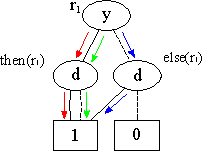
\includegraphics[scale=1.5]{r1_clean_paths.pdf}
\caption*{Paths terminating in 1: ${\color{red} yd}, {\color{green} y}, {\color{blue} d}  $.}
\label{r1}
\end{figure}
  
\end{frame}

\begin{frame}{\large{Improved Reduction Using ZDDs}}
\bi
  \item $r_1=yd + y + d$, $f_2=y + xc + x + c$, $r_1 \xrightarrow{f_2}_+$
  % \item $r_1 = yd + y + d$, ~~$f_2 = y + xc + x + c$
  % \item Quotient$(r_1 \xrightarrow{f_2}_+ r_2) = d+1$
  % \item $r_1 \xrightarrow{f_2}_+ r_2 = $
        {\small
        \begin{align*}
          & (yd + y + d) + (d + 1)\cdot(y + xc + x + c) \pmod{2}\\
          &= 2\cdot(yd + y) + d + (d+1)\cdot(xc + x + c) \pmod{2}\\
          &= \textcolor{green}{d} + (\textcolor{red}{d+1})\cdot(\textcolor{blue}{xc + x + c})  \pmod{2}
        \end{align*}
        }
  % \item This expression provides a formula to compute remainder in one step
\ei
\begin{figure}[hbt]
\centering
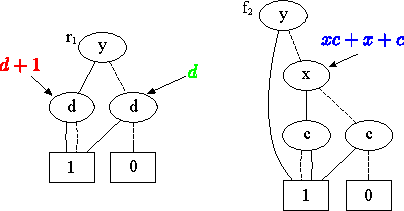
\includegraphics[scale=0.9]{r1_f2_2.pdf}
% \caption{ZDDs for polynomial $r_1$ and $f_2$.}
\label{f2}
\end{figure}
\bi
  \item One step reduction: $else(r_1) + then(r_1)\cdot else(f_2)$
\ei
\end{frame}

\begin{frame}{\large Implementation}
\bi
	\item Custom software: 
	\bi
		\pause
		\vspace{0.1in}
		\item Reduction using ZDDs for remainder generation
		\vspace{0.1in}
		\pause
		\item Singular to compute $P_k(x)$ and model composite field
		\vspace{0.1in}
		\pause
		\item Custom high level finite field engine 
		\pause
		\bi
		\item Bit-vector and coefficient computations
		\item Rectification check
		\ei
	\ei
	\pause
	\item Experiments performed on a 3.5GHz 
	Intel(R) $\text{Core}^{\text{TM}}$ i7-4770K Quad-Core CPU with 32 GB RAM
\ei
\end{frame}

% \begin{frame} {\large Overall Flow}

% \begin{enumerate}
% \item Given Specification $f$, and Circuit $C$ over $\F_{2^n}$
% \item 

% \end{enumerate}

% \end{frame}

\begin{frame}{\large MFR Experiments: Mastrovito}

% \begin{tiny}
% $\textit{n}$ = Datapath Size, $\textit{m}$ = target word size, 
% $\textit{k}$ = composite field size (degree of $P_k(X)$), 
% AM = Maximum resident memory utilization in Mega Bytes,
% \#G = Number of gates $\times 10^3$, \#BO = Number of faulty outputs, 
% PBS = Required time for PolyBori setup (ring declaration/poly collection/spec collection),
% VMS = Required time for verification, polynomial factorization and computing $P_k(X)$, and MFR setup, 
% RC = Required time for MFR check, TE = Required time for total execution
% \end{tiny}

{\scriptsize
\begin{table}[bht]
\centering
\caption*{{\scriptsize $\textit{n}$ = Datapath Size, $\textit{m}$ = target word size, 
$\textit{k}$ = composite field size (degree of $P_k(X)$),\\ 
AM = Maximum resident memory utilization in Mega Bytes,
\#G = Number of gates $\times 10^3$,\\ \#BO = Number of faulty outputs, 
PBS = Required time for PolyBori setup (ring declaration/poly collection/spec collection),
VMS = Required time for verification, polynomial factorization and computing $P_k(X)$, and MFR setup, 
RC = Required time for MFR check, TE = Required time for total execution}}
\label{masvsspec}
\begin{tabular}{| c | c | c | c | c | c | c | c | c | c |} \hline
{\textit{\textbf{n}}} & {\textit{\textbf{m}}} & {\textit{\textbf{k}}} & {\textbf{AM}} & {\textbf{\#G}} 
& {\textbf{\#BO}} & {\textbf{PBS}} & {\textbf{VMS}} & {\textbf{RC}} & {\textbf{TE}} \\ \hline 
16  & 5 & 80   & 100 & 0.8  & 6  & 0.04 & 0.06  & 0.12  & 0.22 \\ \hline
32  & 5 & 160  & 120 & 2.8  & 8  & 0.13 & 0.12  & 0.4   & 0.65 \\ \hline
163 & 5 & 815  & 550 & 69.8 & 6  & 6.04 & 3.36  & 11.9  & 21.3 \\ \hline
233 & 2 & 466  & 750 & 119  & 3  & 13   & 1.2   & 0.01  & 14.2 \\ \hline
283 & 2 & 566  & 1300& 190  & 2  & 38   & 4.2   & 0.1   & 42.3 \\ \hline
409 & 2 & 818  & 2400& 384  & 2  & 190  & 5     & 0.1   & 195  \\ \hline
\rowcolor{green}571 & 2 & 1042 & 5000& 827  & 5  & 2150 & 12    & 0.1   & 2162 \\ \hline
\end{tabular}
\end{table}}

\end{frame}

\begin{frame}{\large MFR Experiments: Montgomery}

{\scriptsize
\begin{table}[bht]
\centering
\caption*{{\scriptsize $\textit{n}$ = Datapath Size, $\textit{m}$ = target word size, 
$\textit{k}$ = composite field size (degree of $P_k(X)$), 
\\AM = Maximum resident memory utilization in Mega Bytes,
\#G = Number of gates $\times 10^3$, \\ \#BO = Number of faulty outputs, 
PBS = Required time for PolyBori setup (ring declaration/poly collection/spec collection),
VMS = Required time for verification, polynomial factorization and computing $P_k(X)$, and MFR setup, 
RC = Required time for MFR check, TE = Required time for total execution}}
\label{montvsspec}
\begin{tabular}{| c | c | c | c | c | c | c | c | c | c |} \hline
{\textit{\textbf{n}}} & {\textit{\textbf{m}}} & {\textit{\textbf{k}}} & {\textbf{AM}} & {\textbf{\#G}} 
& {\textbf{\#BO}} & {\textbf{PBS}} & {\textbf{VMS}} & {\textbf{RC}} & {\textbf{TE}} \\ \hline 
16  & 5 & 80   & 100 & 0.9  & 16  & 0.04 & 0.56 & 35.6     & 36   \\ \hline
32  & 5 & 160  & 120 & 2.8  & 32  & 0.13 & 0.57 & 27.6     & 28.3 \\ \hline
163 & 5 & 815  & 550 & 57.5 & 128 & 5.2  & 6.8  & 262      & 274  \\ \hline
233 & 2 & 466  & 750 & 112  & 233 & 11.5 & 3.5  & 360      & 375  \\ \hline
283 & 2 & 566  & 1300& 171  & 283 & 35   & 11   & 1503     & 1549 \\ \hline
\rowcolor{red}409 & 2 & 818  & 2400& 340  & 409 & 134  & 10   & 4920 & 5064 \\ \hline
\rowcolor{green}571 & 2 & 1042 & 5000& 663  &  12 & 1313 & 82   & 0.2 & 1395 \\ \hline
\end{tabular}
\end{table}}

\end{frame}

\begin{frame}{\large MFR Experiments: Point Addition}

{\scriptsize
\begin{table}[bht]
\centering
\caption*{{\scriptsize $\textit{n}$ = Datapath Size, $\textit{m}$ = target word size, 
$\textit{k}$ = composite field size (degree of $P_k(X)$), 
\\AM = Maximum resident memory utilization in Mega Bytes,
\#G = Number of gates $\times 10^3$, \\ \#BO = Number of faulty outputs, 
PBS = Required time for PolyBori setup (ring declaration/poly collection/spec collection),
VMS = Required time for verification, polynomial factorization and computing $P_k(X)$, and MFR setup, 
RC = Required time for MFR check, TE = Required time for total execution}}
\label{pavsspec}
\begin{tabular}{| c | c | c | c | c | c | c | c | c | c |} \hline
{\textit{\textbf{n}}} & {\textit{\textbf{m}}} & {\textit{\textbf{k}}} & {\textbf{AM}} & {\textbf{\#G}} 
& {\textbf{\#BO}} & {\textbf{PBS}} & {\textbf{VMS}} & {\textbf{RC}} & {\textbf{TE}} \\ \hline 
16 & 5 & 80   & 100 & 0.9  & 7   & 0.06 & 0.11 & 1.73 & 1.9  \\ \hline
32  & 5 & 160  & 120 & 2.9  & 13  & 0.18 & 0.8  & 134  & 135  \\ \hline
163 & 5 & 815  & 550 & 71.6 & 22  & 15.7 & 4.7  & 15   & 35.4 \\ \hline
233 & 2 & 466  & 750 & 122  & 233 & 19.2 & 2.15 & 0.15 & 21.5 \\ \hline
\rowcolor{green}283 & 2 & 566  & 1300& 208  & 4   & 80.4 & 6.1  & 0.1  & 86.6 \\ \hline
\rowcolor{red}409 & 2 & 818  & 2400& 368  & 409 & 220  & 10   & 2007 & 2237 \\ \hline
571 & 2 & 1042 & 5000& 813  & 5   & 2583 & 27   & 880  & 3490 \\ \hline
\end{tabular}
\end{table}}

\end{frame}



% {\tiny
% \begin{table}[]
% \centering
% \caption{{\footnotesize {\footnotesize Time is in seconds; $\textit{n}$ = Datapath Size, $\textit{m}$ = target word size, 
% $\textit{k}$ = composite field size (degree of $P_k(X)$), 
% AM = Maximum resident memory utilization in Mega Bytes,
% \#G = Number of gates $\times 10^3$, \#BO = Number of faulty outputs, 
% PBS = Required time for PolyBori setup (ring declaration/poly collection/spec collection),
% % VF = time for verification (Sec.~\ref{sec:verify}), MS = Multi-fix check setup time (Sec.~\ref{sec:comps} 
% % [Rectification Setup]), RC = time for MFR check (Thm.~\ref{Thm:rect}), TE = Total execution time.}}
% VMS = Required time for verification, polynomial factorization and computing $P_k(X)$, and MFR setup, 
% RC = Required time for MFR check, TE = Required time for total execution}}}
% \label{masusmontspec}
% \begin{tabular}{| c | c | c | c | c | c | c | c | c | c |} \hline
% {\textit{\textbf{n}}} & {\textit{\textbf{m}}} & {\textit{\textbf{k}}} & {\textbf{AM}} 
% & {\textbf{\#G}} & {\textbf{\#BO}} & {\textbf{PBS}} & {\textbf{VMS}} & {\textbf{RC}} & {\textbf{TE}} \\ \hline 
% \mb{16}  & \mb{5} & \mb{80  } & 100 & 0.9  & 7   & 0.06 & 0.11 & 1.73 & 1.9  \\ \hline
% \mb{32 } & \mb{5} & \mb{160 } & 120 & 2.9  & 13  & 0.18 & 0.8  & 134  & 135  \\ \hline
% \mb{64 } & \mb{3} & \mb{192 } & 160 & 10.6 & 64  & 0.84 & 0.56 & 58.1 & 59.5 \\ \hline
% \mb{96 } & \mb{2} & \mb{96  } & 240 & 24.8 & 96  & 2.46 & 0.64 & 14.9 & 18   \\ \hline
% \mb{128} & \mb{2} & \mb{128 } & 370 & 43.2 & 128 & 6.45 & 1.55 & 73   & 81   \\ \hline
% \mb{163} & \mb{5} & \mb{815 } & 550 & 71.6 & 22  & 15.7 & 4.7  & 15   & 35.4 \\ \hline
% \mb{233} & \mb{2} & \mb{466 } & 750 & 122  & 233 & 19.2 & 2.15 & 0.15 & 21.5 \\ \hline
% \mb{283} & \mb{2} & \mb{566 } & 1300& 208  & 4   & 80.4 & 6.1  & 0.1  & 86.6 \\ \hline
% \mb{409} & \mb{2} & \mb{818 } & 2400& 368  & 409 & 220  & 10   & 2007 & 2237 \\ \hline
% \mb{571} & \mb{2} & \mb{1042} & 5000& 813  & 5   & 2583 & 27   & 880  & 3490 \\ \hline
% \end{tabular}
% \end{table}}

% \end{frame}


% \begin{frame}{\large MFR Experiments: Custom software}

% {\tiny
% \begin{table}[]
% \centering
% \caption{{\footnotesize Time is in seconds; $\textit{I}$ = Index, $\textit{n}$ = Datapath Size, $\textit{m}$ = target word size, 
% $\textit{k}$ = composite field size (degree of $P_k(X)$), 
% AM = Maximum resident memory utilization in Mega Bytes,
% \#G = Number of gates $\times 10^3$, \#BO = Number of faulty outputs, 
% PBS = Required time for PolyBori setup (ring declaration/poly collection/spec collection),
% % VF = time for verification (Sec.~\ref{sec:verify}), MS = Multi-fix check setup time (Sec.~\ref{sec:comps} [Rectification Setup]), RC = time for MFR check (Thm.~\ref{Thm:rect}), TE = Total execution time.}}
% VMS = Required time for verification, polynomial factorization and computing $P_k(X)$, and MFR setup, 
% RC = Required time for MFR check, TE = Required time for total execution}}
% \label{mavsspec}
% \resizebox{\linewidth}{!}{
% \begin{tabular}{!{\vrule width 1pt} c | c | c | c | c !{\vrule width 1pt} c | c | c | c | c | c !{\vrule width 1pt} c | c | c | c | c | c !{\vrule width 1pt} c | c | c | c | c | c !{\vrule width 1pt}}\noalign{\hrule height 1pt}
% \multicolumn{5}{!{\vrule width 1pt} c !{\vrule width 1pt}}{} & \multicolumn{6}{ c !{\vrule width 1pt}}{Mastrovito} & \multicolumn{6}{ c !{\vrule width 1pt}}{Montgomery} & \multicolumn{6}{ c !{\vrule width 1pt}}{Point Addition}\\ \noalign{\hrule height 1pt}

% {\textit{I}} & {\textit{\textbf{n}}} & {\textit{\textbf{m}}} & {\textit{\textbf{k}}} & {\textbf{AM}} & {\textbf{\#G}} & {\textbf{\#BO}} & {\textbf{PBS}} & {\textbf{VMS}} & {\textbf{RC}} & {\textbf{TE}}& {\textbf{\#G}} & {\textbf{\#BO}} & {\textbf{PBS}} & {\textbf{VMS}} 
% & {\textbf{RC}} & {\textbf{TE}}& {\textbf{\#G}} & {\textbf{\#BO}} & {\textbf{PBS}} & {\textbf{VMS}} & {\textbf{RC}} & {\textbf{TE}}\\ \noalign{\hrule height 1pt}

% 1  & \mb{16}  & \mb{5} & \mb{80  } & 100 & 0.8  & 6  & 0.04 & 0.06  & 0.12  & 0.22 & 0.9  & 16  & 0.04 & 0.56 & 35.6     & 36   & 0.9  & 7   & 0.06 & 0.11 & 1.73 & 1.9  \\ \hline
% 2  & \mb{32 } & \mb{5} & \mb{160 } & 120 & 2.8  & 8  & 0.13 & 0.12  & 0.4   & 0.65 & 2.8  & 32  & 0.13 & 0.57 & 27.6     & 28.3 & 2.9  & 13  & 0.18 & 0.8  & 134  & 135  \\ \hline
% 3  & \mb{64 } & \mb{3} & \mb{192 } & 160 & 11.2 & 5  & 0.57 & 0.45  & 227   & 228  & 9.6  & 47  & 0.52 & 0.32 & 1.79     & 2.63 & 10.6 & 64  & 0.84 & 0.56 & 58.1 & 59.5 \\ \hline
% 4  & \mb{96 } & \mb{2} & \mb{96  } & 240 & 24.5 & 5  & 1.47 & 0.26  & 0.83  & 2.56 & 21   & 96  & 1.36 & 1.27 & 13.3     & 16   & 24.8 & 96  & 2.46 & 0.64 & 14.9 & 18   \\ \hline
% 5  & \mb{128} & \mb{2} & \mb{128 } & 370 & 43.2 & 5  & 3.23 & 0.5   & 2.03  & 5.76 & 35.8 & 128 & 2.8  & 1.4  & 64.2     & 68.4 & 43.2 & 128 & 6.45 & 1.55 & 73   & 81   \\ \hline
% 6  & \mb{163} & \mb{5} & \mb{815 } & 550 & 69.8 & 6  & 6.04 & 3.36  & 11.9  & 21.3 & 57.5 & 128 & 5.2  & 6.8  & 262      & 274  & 71.6 & 22  & 15.7 & 4.7  & 15   & 35.4 \\ \hline
% 7  & \mb{233} & \mb{2} & \mb{466 } & 750 & 119  & 3  & 13   & 1.2   & 0.01  & 14.2 & 112  & 233 & 11.5 & 3.5  & 360      & 375  & 122  & 233 & 19.2 & 2.15 & 0.15 & 21.5 \\ \hline
% 8  & \mb{283} & \mb{2} & \mb{566 } & 1300& 190  & 2  & 38   & 4.2   & 0.1   & 42.3 & 171  & 283 & 35   & 11   & 1503     & 1549 & 208  & 4   & 80.4 & 6.1  & 0.1  & 86.6 \\ \hline
% 9  & \mb{409} & \mb{2} & \mb{818 } & 2400& 384  & 2  & 190  & 5     & 0.1   & 195  & 340  & 409 & 134  & 10   & 4920*    & 5064 & 368  & 409 & 220  & 10   & 2007 & 2237 \\ \hline
% 10 & \mb{571} & \mb{2} & \mb{1042} & 5000& 827  & 5  & 2150 & 12    & 0.1   & 2162 & 663  &  12 & 1313 & 82   & 0.2$\td$ & 1395 & 813  & 5   & 2583 & 27   & 880  & 3490 \\ \hline\hline
% 11 & \mb{16}  & \mb{7} & \mb{112 } & 100 & 0.8  & 11 & 0.04 & 0.17  & 4.96  & 5.14 & 0.9  & 13  & 0.05 & 2    & 228      & 230  & 0.9  & 12  & 0.05 & 0.55 & 33   & 33.6 \\ \hline
% 12 & \mb{32 } & \mb{5} & \mb{160 } & 120 & 2.8  & 8  & 0.13 & 0.09  & 0.81  & 1.03 & 2.8  & 32  & 0.13 & 0.9  & 100      & 101  & 2.9  & 13  & 0.18 & 0.8  & 244  & 245  \\ \hline
% 13 & \mb{64 } & \mb{3} & \mb{192 } & 160 & 11.2 & 5  & 0.58 & 0.23  & 1.64  & 2.45 & 9.6  & 47  & 0.51 & 0.6  & 10.4     & 11.4 & 10.6 & 5   & 0.8  & 0.2  & 4    & 5 \\ \hline
% 14 & \mb{96 } & \mb{2} & \mb{96  } & 240 & 24.5 & 5  & 1.48 & 0.25  & 0.04  & 1.77 & 21   & 96  & 1.34 & 2.16 & 87.5     & 91   & 24.8 & 96  & 2.44 & 0.66 & 35.5 & 38.6 \\ \hline
% 15 & \mb{128} & \mb{2} & \mb{128 } & 370 & 43.2 & 5  & 3.21 & 0.53  & 0.1   & 3.84 & 35.8 & 128 & 2.7  & 1.3  & 66       & 70   & 43.2 & 128 & 6    &  2   & 73   & 81   \\ \hline
% 16 & \mb{163} & \mb{5} & \mb{815 } & 550 & 69.8 & 6  & 6.3  & 3.4   & 12    & 21.7 & 57.5 & 128 & 5.3  & 7.7  & 524      & 537  & 71.6 & 22  & 16   &  4.6 & 37   & 57.6 \\ \hline
% 17 & \mb{409} & \mb{2} & \mb{818 } & 2400& 384  & 2  & 208  & 4     & 0.03  & 212  & 340  & 13  & 127  & 7.9  & 0.13     & 135  & 368  & 3   & 210  &  8   & 928  & 1146 \\ \hline
% 18 & \mb{571} & \mb{2} & \mb{1042} & 5000& 827  & 5  & 2246 & 10    & 0.11  & 2256 & 663  & 427 & 1358 & 63.8 & 2.24     & 1424 & 813  & 5   & 2433 &  19  & 5    & 2457 \\ \noalign{\hrule height 1pt}
% \end{tabular}
% }
% \end{table}
% }
% \end{frame}

\begin{frame}{\large Conclusion and Future work}
\bi

	\item Algebraic approach for $m$-target MFR checking
	\bi
		\item Efficiency derived by interpreting targets as a bit-vector
	\ei
	\pause
	\item New mathematical insights for unified framework
	\bi
		\item Field incompatibility
		\item Primitive polynomial computation
	\ei
	\pause
	\vspace{0.1in}
	\vspace{0.1in}
	\item Computation of rectification function at the word-level
	\bi
		\item $W = a_2b_1b_2 + \beta \cdot a_2b_2$
		\item $r_3 = (a_2 \wedge b_1 \wedge b_2),~~rr_3 = (a_2 \wedge b_2)$
	\ei
	\pause
	\item Define and formulate existence of don't cares at the word-level
	\pause
	\item Extend the approach to integer arithmetic circuits
\ei
\end{frame}


% \begin{frame}{\large MFR Function Example}
% \bi
% 	\item Compute a rectification function of the form $W = U(X_{PI})$ 
% 	\bi
% 		% \item Here $U$ is the \textit{unknown component} computed as an $m$-bit-vector word
% 		\item $U(X_{PI}) = \sum_{i=0}^{m-1}\be^iu_i$ 
% 		\bi
% 			\item Where $u_i$'s represent the individual Boolean functions for the respective $w_i$'s.
% 		\ei
% 	\ei
% 	\pause
% 	\item A polynomial which can be computed to rectify the circuit
% 	\bi
% 		\item $W = a_2b_1b_2 + \beta \cdot a_2b_2$
% 		\item $r_3 = (a_2 \wedge b_1 \wedge b_2),~~rr_3 = (a_2 \wedge b_2)$
% 	\ei
% 	% \item The \textit{unknown component} problem is then formulated as an ideal membership test and
% 	% solved using extended \Grobner Basis: 
% 	% \begin{center}
% 	% 	\begin{align*}
% 	% 	&W + \be^0 e_0 + \be d_5  = W + U = W +\be^0(a_1b_2+a_2b_1)+\be a_2b_2;\\
% 	% 	&e_0 = a_1b_2+a_2b_1;~~d_5 = a_2b_2;
% 	% 	\end{align*}
% 	% \end{center}
% \ei
% \end{frame}


% \begin{frame}{\large Rectification function computation }

% \bi
% 	\item SFR of finite field arithmetic circuits
% 		[{\it Rao. et al}, FMCAD'18][{\it Rao. et al}, IWLS'18]
% 	\bi
% 		\item Quantification based computation
% 		\item Alternate to Craig Interpolation  
% 	\ei
% \vspace{0.1in}
% \item Currently addressing function computation at a word-level for finite field arithmetic circuits: 
% \bi
% \item Rectification function computation at multiple nets in terms of primary inputs [Due notification GLSVLSI'21]
% \bi
% 	% \item Synthesizing a correction function in terms of primary inputs 
% 	\item Define and formulate existence of don't cares 
% 	\item Devise algorithms to explore don't cares for logic optimization 
% \ei
% \item Formulate rectification setup in terms of internal nets of the circuit. 
% \bi
% 	\item Explore word-level don't care formulation in terms of internal nets.
% \ei
% \item Extend the multi-fix approach to integer arithmetic circuits and address the associated challenges.
% \ei
% \ei
% \end{frame}

% \begin{frame}{\large Objectives}
% \begin{enumerate}
% 	\item Enhance the investigations on MFR of finite field circuits to accommodate the following challenges 
% 	\vspace{0.1in}
% 	\bi
% 		\item Heuristics to identify effective rectification targets
% 		\vspace{0.1in}
% 		\item Rectification setup in terms of internal nets 
% 		\vspace{0.1in}
% 		\item Derive a word-level abstraction model
% 		\bi
% 			\item Address mathematical challenges posed by the word-level formulation
% 		\ei
% 		\vspace{0.1in}
% 		\item Define and formulate existence of don't cares at the word-level
% 		\vspace{0.1in}
% 		\item Devise algorithms to compute efficient low cost patch functions by exploring the don't care setup 
% 	\ei
% \end{enumerate}
% \end{frame}

% \begin{frame}{\large Objectives}
% \begin{enumerate}
% \setcounter{enumi}{1}
% 	\item Extension to integer arithmetic circuits
% 	\bi
% 		\item Formulate the MFR approach 
% 		\item Address the mathematical challenges associated with it  
% 	\ei
% 	\vspace{0.1in}	
% 	\item Improving scalability of the approach
% 	\bi
% 		\item Utilize PolyBori’s reduction procedure with ZDD data structure
% 		\item Develop a computational engine to implement the rectification framework
% 	\ei
% 	\vspace{0.1in}
% 	\item Theory of permissible functions [{\it Muroga. et al} ITC'89][{\it Fujita. et al} IWLS'19] 
% 	\bi
% 		\item Use don't cares for logic optimization
% 	\ei
% \end{enumerate}
% \end{frame}

% 
\begin{frame}{\large Problem Description: Rectification}
\vspace{-0.1in}
\begin{align*}
Z = A\cdot B \pmod{P(X)}
\end{align*}
\vspace{-0.1in}
\begin{figure}[hbt]
\centering
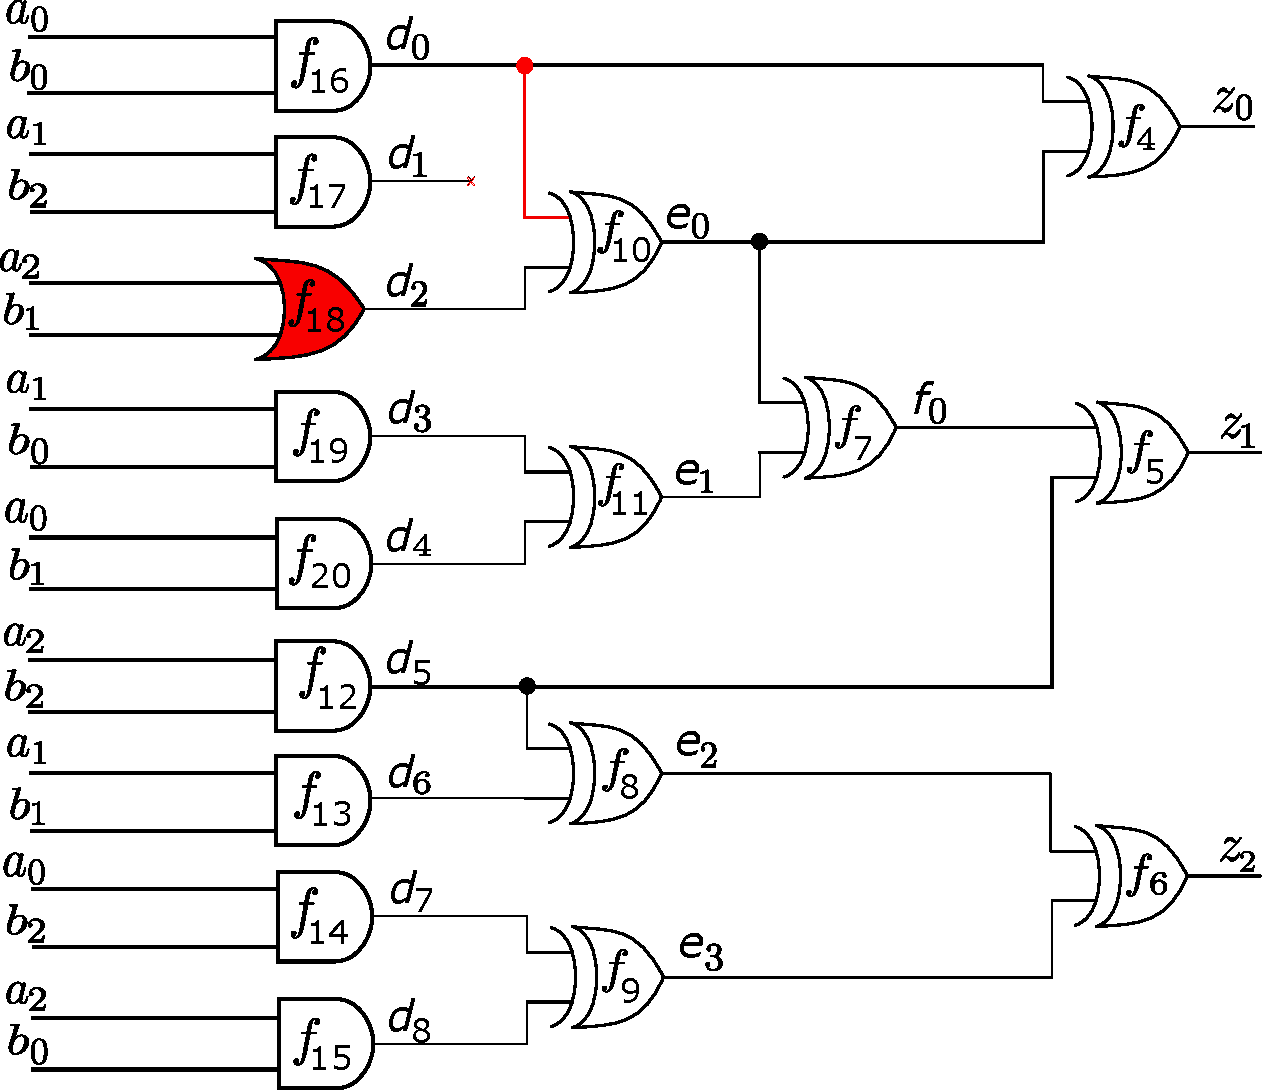
\includegraphics[scale=0.32]{mas_3_sfr.pdf}
\caption*{A buggy implementation of a 3-bit modulo multiplier}
\end{figure}
\end{frame}

\begin{frame}{\large Problem Description: Rectification}
\begin{figure}[hbt]
\centering
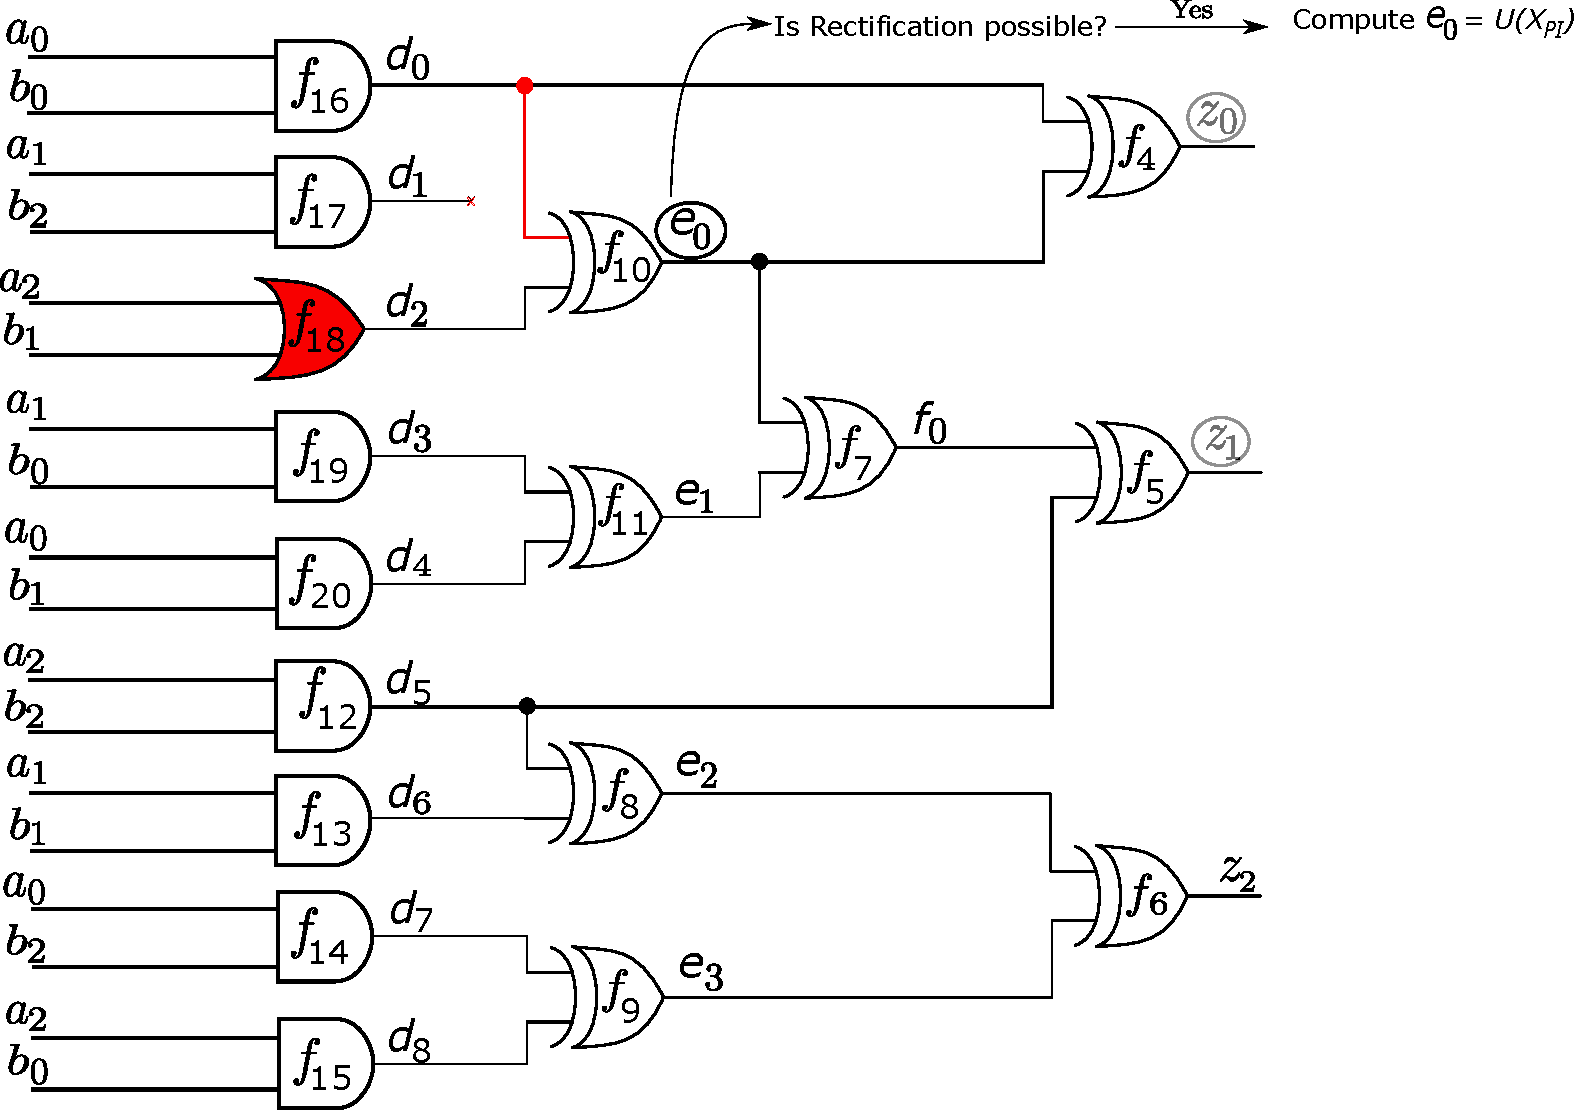
\includegraphics[scale=0.35]{mas_3_sfr2.pdf}
% \caption*{Buggy 2-bit modulo multiplier circuit}
\end{figure}
\end{frame}

\begin{frame}{\large Finite Field Notations}
	\bi
		\item Finite (Galois) Field $\Fq$: 
		\bi
			\item Set of $q$ finitely many elements. $q=p^n$, $p=prime$
		\ei
		\item $\F_2 = \B = \{0,1\}$
		\item On circuits, $p=2$, $n=$ data-operand width 
		\item Hardware cryptography extensively based on $\Fkn$ (we use $\Fkn$)
		\item $\F_2 \subset \Fkn$, $n>1$
		% \item $q = p$ or $q = p^n$ ($k \in \N$); $p$ is a prime
		% \bi
		% 	\item $\F_2$: set of elements 0 and 1
		% 	\item $\F_5$: $\{0,1,2,3,4\}$
		% \ei
		% \item Addition, Multiplication are Associative and Commutative
		% \item $\forall e \in \Fq$ and $e \neq 0$, $\exists e^{-1}$ $s.t. e\cdot e^{-1} = 1$
		% \item Finite (Galois) field $\Fq$ has finitely many elements
		% \item $\F_{p^n}$ ($k \neq 1$) is extension of $\F_p$
		\item Contribution: Application to integer arithmetic circuits
		\bi
			\item Infinite sets: More investigation needed 
		\ei
	\ei
\end{frame}

\begin{frame}{\large Modeling Circuits using Polynomials}
\bi
\item Circuit $C$ modeled as polynomials
\item Boolean logic gates in $\F_2$ ($\F_2 \subset \Fkn$); Over $\F_2$ $-1 = +1 \pmod{2}$)
\begin{align*}
z ~ =  ~ \neg a ~ & \rightarrow ~ z+a+1 \pmod 2  \\
z ~ =  ~ a \wedge b ~ & \rightarrow ~ z+a\cdot b \pmod 2\\
z ~ =  ~ a \vee b ~ & \rightarrow ~ z+a+b+a\cdot b \pmod 2 \\
z ~ =  ~ a \oplus b ~ & \rightarrow ~ z+a+b \pmod 2 
\end{align*}
\item Specification in $\Fkn$, $f_{spec}:Z+AB$
\item Word level polynomials [$\ga=$ Primitive element of $\Fkn$]
\bi
	\item Output: $Z + z_0 +\ga z_1 +\ga^2 z_2 + \cdots +\ga^{n-1} z_{n-1}$,
	\item Input: $A + \sum_{i=0}^{n-1}\ga^ia_i$, and so on
\ei 
\ei
\end{frame}

\begin{frame}{\large Polynomial Ring}
%need to be written in an specific order
%manipulate term-by-term 
\bi
	\item Given $\{x_1,\dots,x_d\}$
	\bi
		\item Monomial $X = x_1^{e_{1}}\cdot x_2^{e_{2}}\cdots x_d^{e_{d}}$, where $e_i \in \Z_{\geq 0}, i\in \{1, \dots,d\}$
		\item Polynomial $f = c_1 X_1 + c_2 X_2 + \dots + c_t X_t$; $c_i \in \Fkn$
	\ei
	\item All such $f$ form the ring $R = \Fkn[x_1,\dots,x_d]$
	% \item Univariate polynomial division, leading term: monomial with highest degree
	\vspace{0.1in}
	\item Multivariate polynomials: need to order the monomials
	\vspace{0.1in}
	\item Impose monomial order ``$>$'' on $R$
	\bi
		\item We utilize \alert{{\it lex}} term order
		% \item lex (for 2 variables, $x_1>x_2$): $x_1^2 >x_1x_2 >x_2^2>x_2>1$ 
	\ei
	\vspace{0.1in}
	\item $f = c_1 X_1 + c_2 X_2 + \dots + c_t X_t$  ~~~(with lex order)
	\bi
		\item $lt(f) = c_1 X_1, ~lm(f) = X_1, ~lc(f) = c_1$
	\ei
\ei
\end{frame}

\begin{frame}{\large Sum, Product, and Quotient of Ideals}
\begin{center}
Given $J_1 = \langle f_1,\dots,f_s\rangle \in R$ and $J_2=\langle h_1,\dots,h_r\rangle \in R$
\end{center}
\bi 
\item Sum of ideals:
\bi
	\item $J_1 + J_2 = \langle f_1,\dots,f_s, h_1\dots,h_r\rangle$
\ei
\item Product of ideals:
\bi
\item $J_1\cdot J_2 = \langle f_i\cdot h_j: 1\leq i\leq s, 1\leq j\leq r\rangle$
\ei

\item Ideal quotient of $J_1$ by $J_2$:
\bi
\item $J_1:J_2 = \{f \in R \ |\ f\cdot h \in J_1, \forall h \in J_2\}$
\ei

\item Ideals and varieties are dual concepts
\bi
\item $V(J_1 + J_2) = V(J_1) \cap V(J_2)$
\item $V(J_1\cdot J_2) = V(J_1) \cup V(J_2)$
\item $V(J_1:J_2) = V(J_1)-V(J_2)$
\ei
% \item Moreover, if $J_1 \subseteq J_2$ then $V(J_1)\supseteq V(J_2)$
\ei

\end{frame}

\begin{frame}{\large Vanishing Ideals} %x^2 - x
% Ensure that var takes values only in $\F_2$
% Boolean values 
\bi
	% \item Fermat's little Theorem: $e \in \Fkk$, $e^{2^k} = e$
	\item For variables in circuit ideals:
	\bi
		\item Bit-level $x_i$: $x_i^2 - x_i$ or $x_i^2 + x_i$ as $-1 = +1\pmod{2}$ over $\Fkn$
		\item Word-level $Z$, $A$: $Z^{2^n} - Z$, $A^{2^n} - A$
	\ei
	\vspace{0.1in}
	\item Vanishing Ideal: $J_0 = \langle F_0 \rangle =  \langle x_1^2+x_1,\dots,x_d^2+x_d, Z^{2^n}+Z, A^{2^n}+A\rangle$
	\vspace{0.1in}
	\item Vanishing Ideal purpose: 
	\bi
		\item Restrict solutions to $x_i$ in $\F_2$
		\item Restrict solutions to $Z,A$ in $\Fkn$
	\ei
	\vspace{0.1in}
	\item For circuits [{\it Lv. et al}, TCAD'13]
	\bi
		% \item vanishing ideals of PIs variables ($\xpi$) required
		\item Only need $\jzpi = \langle \fzpi \rangle = \langle x_i^2 + x_i: x_i \in \xpi \rangle$ added to $J$ 
	\ei
\ei
\end{frame}


\begin{frame}{\large MFR Notations: Composite Field}
\bi
	\item For a given circuit with data-path size $n$
	\bi
		\item Polynomials modeled over $R=\Fkn[Z,A,x_1,\dots,x_d]$
		\bi
			\item $\{x_1, \dots$ $, x_d\}$ are all the bit-level variables (nets) in the circuit
			\item $Z$ and $A$ are the word-level output and input, respectively
		\ei
		\item $\Fkn$ is constructed as $\Fkn = \Ftwo[X]\pmod{P_n(X)}$
		\bi
			\item $P_n(X) \in \F_2[X]$ is a given degree-$n$ primitive polynomial; $P_n(\ga) =0$ 
			% [$\ga$ as one of its root].
		\ei
		\item  The word-level polynomials for $Z,A$ are modeled as:
		\bi
			\item $f_z: Z + \sum_{i=0}^{n-1}\ga^iz_i;f_a: A + \sum_{i=0}^{n-1}\ga^ia_i;$ 
		\ei
	\ei 
	\item Patch $W$ for $m$ targets is computed as a polynomial function in the field $\Fkm$
	\bi
		\item $\Fkm$ is constructed as $\Fkm = \Ftwo[X]\pmod{P_m(X)}$
		\bi
			\item We select a degree-$m$ primitive polynomial $P_m(X)\in \F_2[X]$; $P_m(\be) =0$ 
			% [$\be$ as one of its root].
		\ei
		\item  The word-level polynomial for $W$ is modeled as:
		\bi
			\item $f_w: W + \sum_{i=0}^{m-1}\be^iw_i$
			\item $\{w_0,\dots,w_{m-1}\} \subset \{x_1,\dots,x_d\}$
		\ei
	\ei
\ei
\end{frame}

\begin{frame}{\large MFR Notations: Composite Field}
\bi
	\item Determine the smallest single field ($\Fkk$) to operate both circuit ($\Fkn$) and patch ($\Fkm$)
	\vspace{0.1in}
	\item Smallest $k$ is $LCM(n,m)$
	\bi
		\item $\Fkk \supset \Fkn$ and $\Fkk \supset \Fkm$
		\item $\Fkk$ is constructed as $\Fkk = \Ftwo[X]\pmod{P_k(X)}$
		\bi
			\item $P_k(X)$ is a degree-$k$ primitive polynomial; $P_k(\al) =0$ 
		\ei
	\ei
	\vspace{0.1in}
	\item  Mathematical challenge: Given $P_n(X)$ and $P_m(X)$, compute $P_k(X)$ such that
	$P_n(\ga)= P_m(\be)=P_k(\al)=0$
	\vspace{0.1in}
	\bi
		\item $\ga = \al^{(2^k-1)/(2^n-1)} = \al^{\lambda}$
		\item $\be = \al^{(2^k-1)/(2^m-1)} = \al^{\mu}$
	\ei
	\vspace{0.1in}
	\item Solved using factorization of univariate polynomials over finite fields
\ei

\end{frame}

\begin{frame}{\large MFR Notations: Univariate Polynomial factorization (UPF) }
\bi
	\item Given a monic univariate polynomial $f \in \F_q[X]$, where $\F_q$ is any finite field
	\vspace{0.1in}
	\bi 
		\item Find a complete factorization $f = f_1^{e_1}\cdot f_2^{e_2}\cdots f_l^{e_l}$ 
		\bi
			\item Where $f_1, f_2,\dots, f_l$ are pairwise distinct monic 
			irreducible polynomials in $\F_q[X]$ and $e_1,\dots,e_l$ are positive integers.
		\ei
	\ei
	\vspace{0.1in}
	% \item We employ existing implementation of UPF from computer algebra tool {\it SINGULAR} 
\ei
\end{frame}

\begin{frame}{\large MFR Notations: Finding Primitive Polynomial $P_k(X)$}
\bi
	\item Obtain UPFs of $P_n(X^{\lambda})$ and $P_m(X^{\mu})$
	\bi
		\item Coefficients will be in $\Ftwo$ and degrees will be less than $\lambda$ and $\mu$, respectively.
		\bi
			\item $P_n(X^{\lambda})=P_{n1}^{a1}\cdot P_{n2}^{a2}\cdots P_{nl}^{al}$, and 
			\item $P_m(X^{\mu}) = P_{m1}^{b1}\cdot P_{m2}^{b2}\cdots P_{mg}^{bg}$
		\ei
	\ei
	\vspace{0.1in}
	\item Conjecture: $\exists P_{ni}(X) \in \{P_{n1}, P_{n2},\dots ,P_{nl}\}$ and $\exists P_{mj}(X) \in \{P_{m1}, P_{m2},\dots ,P_{mg}\}$, such that:
	\bi
		\item $P_k(X) = P_{ni}(X)=P_{mj}(X)$,
		\item $P_{k}(X)$ is a degree-$k$ primitive polynomial in $\F_2[X]$ such that $P_k(\al)=0$
	\ei
\ei
\end{frame}


\begin{frame}{\large MFR Application: Verification}
\bi
	\item Circuit designed using irreducible polynomial $P(X) = X^3+X+1$ with $P(\ga)=0$
	\item Denote polynomial $f: Z + A\cdot B$ as the design specification.
	\item Impose RTTO $>$
	\[ \begin{array}{ll}%
f_1:Z + z_0 +\ga z_1 + \ga^2 z_2;   & f_{11}:e_1 + d_3 + d_4; \\       
f_2:A + a_0 +\ga a_1 + \ga^2 a_2;   & \red{f_{12}:d_5 + a_2 + b_2}; \\
f_3:B + b_0 +\ga b_1 + \ga^2 b_2;   & f_{13}:d_6 + a_1b_1; \\          
f_4:z_0 + e_0 + d_0;                & f_{14}:d_7 + a_0b_2; \\          
f_5:z_1 + f_0 + d_5;                & f_{15}:d_8 + a_2b_0; \\          
f_6:z_2 + e_2 + e_3;         & f_{16}:d_0 + a_0b_0; \\
f_7:f_0 + e_0 + e_1;         & f_{17}:d_1 + a_1b_2; \\
f_8:e_2 + d_5 + d_6;         & \red{f_{18}:d_2 + a_2 + b_1 + a_2b_1}; \\
f_9:e_3 + d_7 + d_8;         & f_{19}:d_3 + a_1b_0; \\
\red{f_{10}:e_0 + d_0 + d_2};&    f_{20}:d_4 + a_0b_1;   \\
\end{array}\]%
\ei
\end{frame}

\begin{frame}{\large MFR Application: Verification}
\bi
	\item Polynomial Set
	\bi
		\item $F = \{f_1,\dots,f_{20}\}$ 
		\item $F_0^{PI} = \{a_0^2-a_0, a_1^2-a_1,a_2^2-a_2,b_0^2-b_0, b_1^2-b_1,b_2^2-b_2\}$
	\ei
	\vspace{0.1in}
	\item $f\xrightarrow{F,F_{0}^{PI}}_+= \ga^2(a_2b_2+a_2+b_2)+\ga(a_0b_0+a_1b_2+b_1+a_2b_2+b_2) + (1)(a_0b_0+a_1b_2+b_1+a_2)$
	\vspace{0.1in}
	\item Set of affected outputs: $\Oa = \{z_0,z_1,z_2\}$
	\vspace{0.1in}
	\item Intersection of set of nets in fan-in cones of $\Oa$ is $\emptyset$
	\bi
		\item Implies no SFR points
	\ei
	\vspace{0.1in}
	\item We select $m$=2 and see if the circuit can be rectified by changing
	functions at two nets
\ei
\end{frame}

\begin{frame}{\large MFR Application: Selecting $m$ Targets}
\bi
	\item Since all the outputs are affected, all the nets in the circuit are
	initial candidate targets
	\bi
		\item $\In = \{z_0,z_1,z_2,f_0,e_2,e_3,e_0,e_1,d_5,d_6,d_7,d_8,d_0,d_2,d_3,d_4\}$
		\item Associate a cost for each net driven by synthesis constraints
		\bi
			\item Nets which lie in the intersection of multiple outputs are assigned lowest cost
			\item Rest of the nets are assigned cost based on their topological level in the design
			\item $\Ic = \{4,4,4,3,2,2,-2,2,-2,1,1,1,-2,-2,1,1\}$
		\ei
	\ei
	\vspace{0.1in}
	\item Solved as weighted set cover problem
	\bi 
		\item Partition $\Oa$ into $m$ distinct non-empty subsets such that
		\bi
			\item Intersection of fan-in cones of output bits within a subset is non-empty
		\ei
		\item If such a cover $\M$ exists ($|\M|= m$), each of the $m$ targets are selected from the 
			$m$ distinct covers
		\bi
			\item {\small $\Oa = \{\{z_0,z_1\},\{z_2\}\}$}
			\item {\small $\M = \{\M_0:\{e_0,d_0,d_2\},\M_1:\{d_5,d_6,d_7,d_8,e_2,e_3,z_2\}\}$}
		\ei
	\ei
\ei
\end{frame}


\begin{frame}{\large MFR Application: Word-level Formulation}
\bi
	\item Update ring properties 
	\bi
		\item $R=\F_q[x_1,\dots,x_d,Z,A,W]$
		\item Modify RTTO $>$ to place the target $W$ before the lowest indexed target $e_0$
		\bi
			\item $\{Z\}>\{A>B\}>\{z_0>z_1>z_2\}>\{f_0>e_2>e_3\}>\{{\bf{W}}>e_0>e_1>d_5>d_6>d_7>d_8\}>
				\{d_0>d_1>d_2>d_3>d_4\}>\{a_0>a_1>a_2>b_0>b_1>b_2\}.$
		\ei
	\ei
	\vspace{0.1in}
	\item Update polynomial set $F$ to $F'$:
	\bi
		\item Delete polynomials for $w_i$'s
		\item Delete polynomials in the transitive fan-in of $w_i$'s only
		\item Transitive fan-outs of $w_i$'s need to be replaced with their equivalent 
		word-level representations in terms of $W$
		\item Add $f_w: W + \sum_{i=0}^{m-1}\be^iw_i$
	\ei

\ei
\end{frame}

\begin{frame}{\large MFR Application: Computing $P_k(X)$}
\bi
	\item Composite field: $k=LCM(2,3)=6$
	\vspace{0.1in}
	\bi
		\item $UPF(P_3(X^9)) = \{{\bf X^6+X^4+X^3+X+1},X^6+X^4+X^2+X+1,{\bf X^6+X^5+1}, X^6+X^5+X^2+X+1\}$
		\vspace{0.1in}
		\item $UPF(P_2(X^{21})) = \{{\bf X^6+X^4+X^3+X+1}, {\bf X^6+X^5+1}, X^6+X^3+1, X^6+X^5+X^2+X+1, X^6+X^5+X^3+X^2+1, X^6+X+1, X^6+X^5+X^4+X+1 \}$
		\vspace{0.1in}
		\item We will pick $P_6(X)=X^6+X^4+X^3+X+1$ as the primitive polynomial to setup the unified framework.
	\ei
\ei
\end{frame}

\begin{frame}{\large MFR Notations: Incorrect Primitive Polynomial}
\bi
	\item Note that if we incorrectly choose $P_k(X)=X^6+X^3+1$
	\item For its root $\al$, we have
	\begin{center}
		$\al^6+\al^3+1=0$\\
		$(\al^3)(\al^6+\al^3+1)=0$ (multilying by $\al^3$)\\
		$\al^9+\al^6+\al^3=0$\\
		$\ga+1=0$\label{ga_val}
	\end{center}
	\item But we have $\ga=\al^9$
	\item Selecting arbitrary $P_k(X)$ leads to erroneous results
\ei
\end{frame}

\begin{frame}{\large MFR Application: Word-level Formulation }
\bi
	\item 2-bit rectification patch over the 3-bit circuit can be performed over the field $\F_{2^6}$
	\bi
		\item Field $\F_{2^6} = \F_2[X]$ (mod $P_6(X)$)
	\ei
	\vspace{0.1in}
	\item Update polynomial set $F$ to $F'$ as:
	\begin{center}
		\begin{align*}
			F'=\{f_1,\dots,f_3,f'_4,f'_5,f_6,f'_7,f'_8,f_9,f_w,f_{11},f_{13}\dots,f_{20}\}
		\end{align*}
		{\small\begin{flalign*}
			f'_4:z_0 + (\be W^2 +\be^2 W) + d_0;     &\quad f'_5:z_1 + f_0 + (W^2+W); \\
			f'_7:f_0 + (\be W^2 +\be^2 W) + e_1;   &\quad f'_8:e_2 + (W^2+W) + d_6; \\
			f_w:W + e_0 + \be d_5;             &\quad \be=\al^{21} ; \ga=\al^9;
		\end{flalign*}}
	\end{center}

\ei
\end{frame}

\begin{frame}{\large MFR Contribution: Rectification Check}
%ATPG V() V() = empty
%we have an algebraic proof which is there in the proposal
\bi
	\item Multi-fix rectification at target $W$
	\vspace{0.1in}
	\bi
		\item Construct the following ideals:
		\bi
			\item {\small $J_i = \langle F'_i\rangle =\{f'_1,\dots,f_w=W+\delta(i),\dots,f'_s\}$}
				:$1 \leq i \leq 2^m$, $\delta(0)=0, \delta(1)=1,\delta(2)=\be,\dots,\delta(2^m)= \be^{2^m-2}$
		\ei
		\vspace{0.1in}
		\item Performing the reductions for all $1 \leq i \leq 2^m$: 
		\bi
			\item $f\xrightarrow{F'_i, F_{0}^{PI}}_+r_i $
		\ei
		\item Let $V_{\Fq}(r_i)$ denote the varieties of the respective $r_i$'s
		\vspace{0.1in}
		\item Multi-fix rectification exists at target $W$: \\ 
				\centering
				{\bf if and only if} $\bigcup\limits_{i=1}^{2^m}V_{\Fq}(r_i) = \Fq^{|X_{PI}|} = V(J_0^{PI})$
	\ei
\ei
\end{frame}

\begin{frame}{\large MFR Application: Rectification Check}
\bi
	\item Constructing the $J_i$ ideals:
	\bi
		\item {\small$J_1 = \langle F'_1\rangle$, where $F'_1[f_w]=W+\delta(1)=W$},
		\item {\small$J_2 = \langle F'_2\rangle$, where $F'_2[f_w]=W+\delta(2)=W+1$},
		\item {\small$J_3 = \langle F'_3\rangle$, where $F'_3[f_w]=W+\delta(3)=W+\be$},
		\item {\small$J_4 = \langle F'_4\rangle$, where $F'_4[f_w]=W+\delta(4)=W+\be^2$}
	\ei
	\vspace{0.1in}
	\item Reducing the specification $f: Z+A\cdot B$ modulo these ideals, we get:
	\bi
		\item $r_1 = f \xrightarrow[]{F'_1,F_{0}^{PI}}_+{a_1b_2\ga^3+a_2b_1\ga^3+\ga^4a_2b_2}$
		\item $r_2 = f \xrightarrow[]{F'_2,F_{0}^{PI}}_+{a_1b_2\ga^3+a_2b_1\ga^3+\ga^4a_2b_2+\ga^3}$
		\item $r_3 = f \xrightarrow[]{F'_3,F_{0}^{PI}}_+{a_1b_2\ga^3+a_2b_1\ga^3+\ga^4a_2b_2+\ga^4}$
		\item $r_4 = f \xrightarrow[]{F'_4,F_{0}^{PI}}_+{a_1b_2\ga^3+a_2b_1\ga^3+\ga^4a_2b_2+\ga^6}$
	\ei
	\item Computing $GB(r_1\cdot r_2 \cdot r_3 \cdot r_4, F_{0}^{PI})=F_{0}^{PI}$
	\item Target $W$ with nets $e_0$ and $d_5$ admits MFR
\ei
\end{frame}

\begin{frame}{\large MFR Notation: Computing Rectification Function}
\bi
	\item Compute a rectification function of the form $W = U(X_{PI})$ 
	\bi
		\item Here $U$ is the \textit{unknown component} computed as an $m$-bit-vector word
		\item It represents the function $W = \sum_{i=0}^{m-1}\be^iu_i$ 
		\bi
			\item Where $u_i$'s represent the individual Boolean functions for the respective $w_i$'s.
		\ei
	\ei
	\item The \textit{unknown component} problem is then formulated as an ideal membership test and
	solved using extended \Grobner Basis: 
	\begin{center}
		\begin{align*}
		&W + \be^0 e_0 + \be d_5  = W + U = W +\be^0(a_1b_2+a_2b_1)+\be a_2b_2;\\
		&e_0 = a_1b_2+a_2b_1;~~d_5 = a_2b_2;
		\end{align*}
	\end{center}
\ei
\end{frame}

\begin{frame}{\large Research Objective: Synthesis of Rectification Function}
\bi
	\item Exploring don't cares
	\bi
		\item We computed $U=b_0$, i.e. $f_{10} = e_3 + b_0$
		\item We utilized quotient of ideals to compute alternate corrections
		\bi
			\item ${U^1} = a_1*b_0$
			\item ${U^2} = a_1*b_1*b_0+a_1*b_1+a_1$
		\ei
		\item Polynomial $U$ depends on the polynomial $h_i$ (quotient of division by target $x_i$) 
		\item $h_i$ actually represents the ODCs for the selected target $x_i$
	\ei
	\item Algorithmic computation of rectification polynomials
	\item word-level formulation of don't cares
\ei
\end{frame}



\begin{frame}{\large Research Objective: Integer arithmetic circuits}
\bi
	\item Techniques valid over fields are inapplicable over rings
	\item \Grobner basis and division algorithms are complicated
	\item Can be modeled over $\Q$
	\bi
		\item Rectification function computation can result in {\it fractional coefficients}
		\item Extracting Boolean rectification function requires exhaustive simulation
		\item No scope of optimization as Extended \Grobner basis technique gives zero control
	\ei
\ei

\end{frame}

\begin{frame}{\large Research Objective: Improving Scalability}
\bi
	\item Enhance implementation for finite field circuits:
	\bi
		\item Rectification formulation in terms of internal nets
		\item Address word-level formulation and the mathematical challenges
		\item Devise efficient algorithms based on ZDDs
	\ei
	\vspace{0.2in}
	\item Implementation for Integer arithmetic circuits
	\bi
		\item Bit level reduction technique increases the verification time exponentially
		\bi
			\item No monomial cancellations across output bits
		\ei
		\item Need implicit data structure with a word-level representation
	\ei
	% \item Objective: Compute Boolean polynomials $U_{ON}$, $U_{OFF}$, and $U_{DC}$
	% \bi
	% 	\item Explore don't cares from quotient of division
	% 	\item Formulate as reductions in $\F_2$
	% 	\item Use ZDDs for the computations
	% \ei
	% \item $J_L + \jzpi$ contains:
	% \bi
	% 	\item Miter Polynomial, $f_m : t(Z-Z_S)-1 = tZ-tZ_S-1$ 
	% 	\item Specification Polynomial, $f_{spec} : Z_S + \mathcal{F}(A)$
	% 	\item $Z+\sum_{i=0}^{k-1}z_i\alpha^i,~ A + \sum_{i=0}^{k-1}a_i\alpha^i$, and so on.
	% 	\item Polynomials from logic gates except $f_i$
	% 	\item Vanishing polynomials $x_i^2 + x_i: x_i \in \xpi$
	% \ei
\ei
\end{frame}

% \begin{frame}
% \bi
% 		\item Application to ECOs and Approximate circuits
% 		\bi
% 			\item Current circuit implementation should be minimally 
% 			modified (rectified) to match the ECO-evolved/approximate specification
% 		\ei
% \ei
% \end{frame}
%%%%%%%%%%%%%%%%%%%%%%%%%%%%%%%%%%%%%%%%%%%%%%%%%%


% \begin{frame}{\large Research Objective: To make the approach scalable}
% \bi
% 	\item Exploited ZDDs for bit-level $GB$ reduction (for verification)
% 	\bi
% 		\item Many orders of magnitude improvement
% 	\ei
% 	\item Utilize ZDD based reduction for $GB$ computations in our approach
% \ei
% \end{frame}

% \begin{frame}{\large Proposed Timeline}
% \begin{itemize}
% 	\item Current status: 
% 	\bi
% 	\item Preliminary investigations on single-fix rectification 
% 	\item Result on Craig Interpolants. 
% 	\item Use of interpolants to compute rectification function
% 	\item Experiments on finite field arithmetic benchmarks
% 	\ei
% 	\item Fall 2018: \begin{itemize}
% 			\item Algorithms to explore the interpolant lattice to obtain low-cost rectification functions 
% 			\item Improve the scalability of the procedure. \\
% 			Investigate the use of ZDD based reduction procedure 
% 			\end{itemize}
% \end{itemize}
% \end{frame}
% \begin{frame}{\large Proposed Timeline}
% \bi
% 	\item Spring/Summer 2019: \begin{itemize}
% 	\item Compute rectification functions in internal circuit variables 
% 	\item Investigate extension to multi-fix rectification
% 	\end{itemize}
% 	\item Fall 2019: Evaluate data. Write and defend the dissertation. 
% \ei
% \end{frame}


%!TEX root = UG_PhD_Defense.tex

\begin{frame}[allowframebreaks]{\large Publications}

\begin{thebibliography}{1}
{\small

\bibitem{vikas:fmcad18}
V.~{Rao}, U.~{Gupta}, I.~{Ilioaea}, A.~{Srinath}, P.~{Kalla}, and F.~{Enescu},
  ``{Post-Verification Debugging and Rectification of Finite Field Arithmetic
  Circuits using Computer Algebra Techniques},'' in \emph{Formal Methods in
  Computer Aided Design (FMCAD)}, Oct 2018, pp. 1--9.

\bibitem{Vkrao:IWLS18}
V.~Rao, U.~Gupta, I.~Ilioaea, P.~Kalla, and F.~Enescu, ``{R}esolving {U}nknown
  {C}omponents in {A}rithmetic {C}ircuits using {C}omputer {A}lgebra {M}ethods
  - poster presentation,'' in \emph{{I}nternational {W}orkshop on {L}ogic and
  {S}ynthesis(IWLS)}, 2018.

\bibitem{utkarsh:book-chapter}
U.~Gupta, I.~Ilioaea, V.~Rao, A.~Srinath, P.~Kalla, and F.~Enescu,
  ``{Rectification of Arithmetic Circuits with Craig Interpolants in Finite
  Fields},'' in \emph{{VLSI-SoC: Design and Engineering of Electronics Systems
  Based on New Computing Paradigms}}.\hskip 1em plus 0.5em minus 0.4em\relax
  Springer International Publishing, June 2019, vol. 561, ch.~5, pp. 79--106.

\bibitem{Utkarsh:VLSI18}
------, ``{On the Rectifiability of Arithmetic Circuits using Craig
  Interpolants in Finite Fields},'' in \emph{IFIP/IEEE Intl. Conf. on VLSI
  (VLSI-SoC)}, Oct 2018, pp. 49--54.

\bibitem{utkarsh:tcad17}
U.~Gupta, P.~Kalla, and V.~Rao, ``{Boolean Gr\"obner Basis Reductions on Finite
  Field Datapath Circuits Using the Unate Cube Set Algebra},'' \emph{IEEE
  Trans. on CAD of Integrated Circuits and Systems}, vol.~38, no.~3, pp.
  576--588, Mar 2019.

\bibitem{Utkarsh:IWLS18}
U.~Gupta, I.~Ilioaea, P.~Kalla, F.~Enescu, V.~Rao, and A.~Srinath, ``{C}raig
  {I}nterpolants in {F}inite {F}ields using {A}lgebraic {G}eometry: {T}heory
  and {A}pplications,'' in \emph{Intl. Workshop on Logic and Synthesis (IWLS)},
  June 2018, pp. 70--77.

\bibitem{utkarsh:iwls17}
U.~Gupta, P.~Kalla, and V.~Rao, ``{Boolean Gr\"obner Basis Reductions on
  Datapath Circuits Using the Unate Cube Set Algebra},'' in 
  \emph{International Workshop on Logic \& Synthesis}, pp. 124--131.

}
\end{thebibliography}

% \nocite{Utkarsh:ETS19,utkarsh:book-chapter,Utkarsh:VLSI18,vikas:fmcad18,utkarsh:tcad17,Utkarsh:IWLS18,utkarsh:iwls17}

\end{frame}


\begin{frame}{\ }
\begin{center}
{\bf \Large THANK YOU!} \\ \ \\  
Questions?
\end{center}
\end{frame}

% 
\begin{frame}{\large Problem Description: Rectification}
\vspace{-0.1in}
\begin{align*}
Z = A\cdot B \pmod{P(X)}
\end{align*}
\vspace{-0.1in}
\begin{figure}[hbt]
\centering
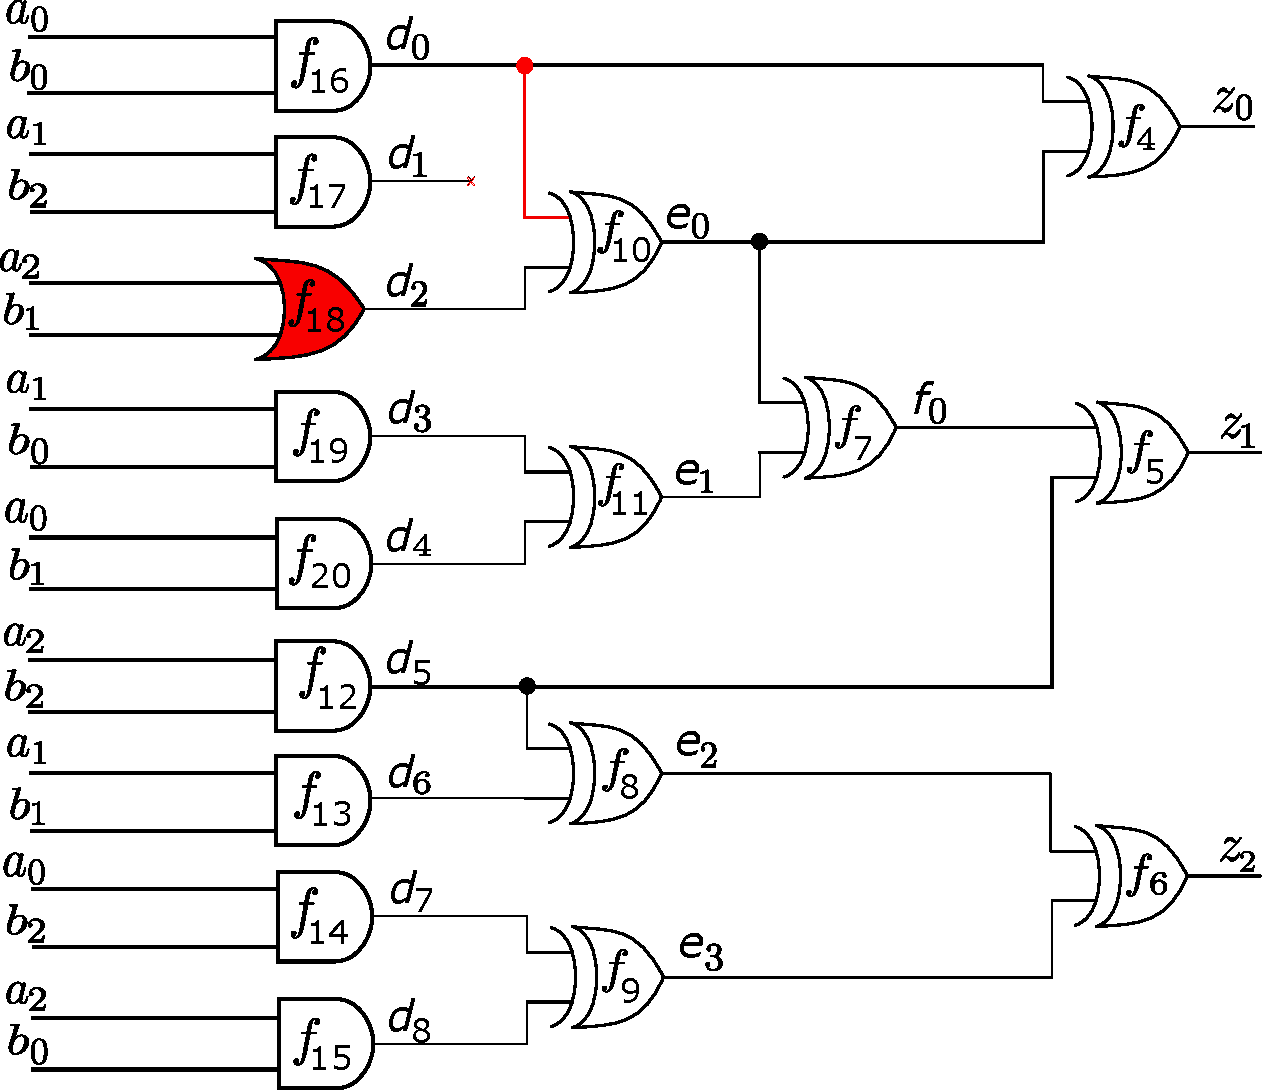
\includegraphics[scale=0.32]{mas_3_sfr.pdf}
\caption*{A buggy implementation of a 3-bit modulo multiplier}
\end{figure}
\end{frame}

\begin{frame}{\large Problem Description: Rectification}
\begin{figure}[hbt]
\centering
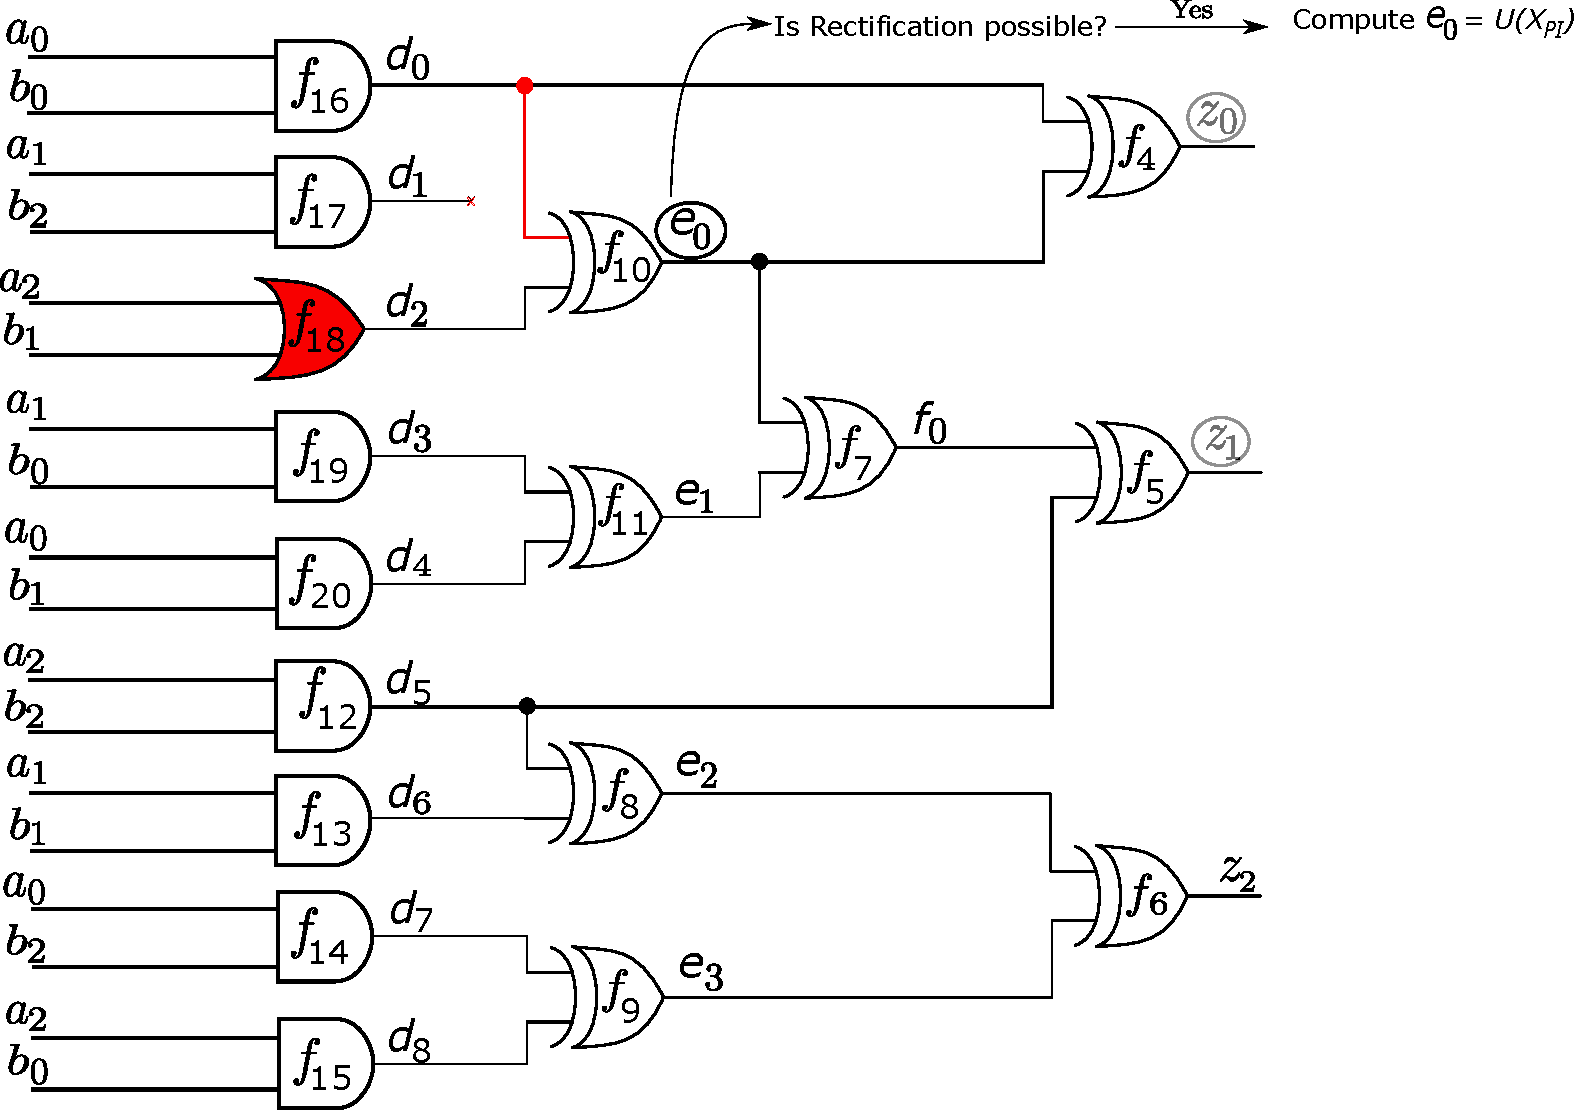
\includegraphics[scale=0.35]{mas_3_sfr2.pdf}
% \caption*{Buggy 2-bit modulo multiplier circuit}
\end{figure}
\end{frame}

\begin{frame}{\large Finite Field Notations}
	\bi
		\item Finite (Galois) Field $\Fq$: 
		\bi
			\item Set of $q$ finitely many elements. $q=p^n$, $p=prime$
		\ei
		\item $\F_2 = \B = \{0,1\}$
		\item On circuits, $p=2$, $n=$ data-operand width 
		\item Hardware cryptography extensively based on $\Fkn$ (we use $\Fkn$)
		\item $\F_2 \subset \Fkn$, $n>1$
		% \item $q = p$ or $q = p^n$ ($k \in \N$); $p$ is a prime
		% \bi
		% 	\item $\F_2$: set of elements 0 and 1
		% 	\item $\F_5$: $\{0,1,2,3,4\}$
		% \ei
		% \item Addition, Multiplication are Associative and Commutative
		% \item $\forall e \in \Fq$ and $e \neq 0$, $\exists e^{-1}$ $s.t. e\cdot e^{-1} = 1$
		% \item Finite (Galois) field $\Fq$ has finitely many elements
		% \item $\F_{p^n}$ ($k \neq 1$) is extension of $\F_p$
		\item Contribution: Application to integer arithmetic circuits
		\bi
			\item Infinite sets: More investigation needed 
		\ei
	\ei
\end{frame}

\begin{frame}{\large Modeling Circuits using Polynomials}
\bi
\item Circuit $C$ modeled as polynomials
\item Boolean logic gates in $\F_2$ ($\F_2 \subset \Fkn$); Over $\F_2$ $-1 = +1 \pmod{2}$)
\begin{align*}
z ~ =  ~ \neg a ~ & \rightarrow ~ z+a+1 \pmod 2  \\
z ~ =  ~ a \wedge b ~ & \rightarrow ~ z+a\cdot b \pmod 2\\
z ~ =  ~ a \vee b ~ & \rightarrow ~ z+a+b+a\cdot b \pmod 2 \\
z ~ =  ~ a \oplus b ~ & \rightarrow ~ z+a+b \pmod 2 
\end{align*}
\item Specification in $\Fkn$, $f_{spec}:Z+AB$
\item Word level polynomials [$\ga=$ Primitive element of $\Fkn$]
\bi
	\item Output: $Z + z_0 +\ga z_1 +\ga^2 z_2 + \cdots +\ga^{n-1} z_{n-1}$,
	\item Input: $A + \sum_{i=0}^{n-1}\ga^ia_i$, and so on
\ei 
\ei
\end{frame}

\begin{frame}{\large Polynomial Ring}
%need to be written in an specific order
%manipulate term-by-term 
\bi
	\item Given $\{x_1,\dots,x_d\}$
	\bi
		\item Monomial $X = x_1^{e_{1}}\cdot x_2^{e_{2}}\cdots x_d^{e_{d}}$, where $e_i \in \Z_{\geq 0}, i\in \{1, \dots,d\}$
		\item Polynomial $f = c_1 X_1 + c_2 X_2 + \dots + c_t X_t$; $c_i \in \Fkn$
	\ei
	\item All such $f$ form the ring $R = \Fkn[x_1,\dots,x_d]$
	% \item Univariate polynomial division, leading term: monomial with highest degree
	\vspace{0.1in}
	\item Multivariate polynomials: need to order the monomials
	\vspace{0.1in}
	\item Impose monomial order ``$>$'' on $R$
	\bi
		\item We utilize \alert{{\it lex}} term order
		% \item lex (for 2 variables, $x_1>x_2$): $x_1^2 >x_1x_2 >x_2^2>x_2>1$ 
	\ei
	\vspace{0.1in}
	\item $f = c_1 X_1 + c_2 X_2 + \dots + c_t X_t$  ~~~(with lex order)
	\bi
		\item $lt(f) = c_1 X_1, ~lm(f) = X_1, ~lc(f) = c_1$
	\ei
\ei
\end{frame}

\begin{frame}{\large Sum, Product, and Quotient of Ideals}
\begin{center}
Given $J_1 = \langle f_1,\dots,f_s\rangle \in R$ and $J_2=\langle h_1,\dots,h_r\rangle \in R$
\end{center}
\bi 
\item Sum of ideals:
\bi
	\item $J_1 + J_2 = \langle f_1,\dots,f_s, h_1\dots,h_r\rangle$
\ei
\item Product of ideals:
\bi
\item $J_1\cdot J_2 = \langle f_i\cdot h_j: 1\leq i\leq s, 1\leq j\leq r\rangle$
\ei

\item Ideal quotient of $J_1$ by $J_2$:
\bi
\item $J_1:J_2 = \{f \in R \ |\ f\cdot h \in J_1, \forall h \in J_2\}$
\ei

\item Ideals and varieties are dual concepts
\bi
\item $V(J_1 + J_2) = V(J_1) \cap V(J_2)$
\item $V(J_1\cdot J_2) = V(J_1) \cup V(J_2)$
\item $V(J_1:J_2) = V(J_1)-V(J_2)$
\ei
% \item Moreover, if $J_1 \subseteq J_2$ then $V(J_1)\supseteq V(J_2)$
\ei

\end{frame}

\begin{frame}{\large Vanishing Ideals} %x^2 - x
% Ensure that var takes values only in $\F_2$
% Boolean values 
\bi
	% \item Fermat's little Theorem: $e \in \Fkk$, $e^{2^k} = e$
	\item For variables in circuit ideals:
	\bi
		\item Bit-level $x_i$: $x_i^2 - x_i$ or $x_i^2 + x_i$ as $-1 = +1\pmod{2}$ over $\Fkn$
		\item Word-level $Z$, $A$: $Z^{2^n} - Z$, $A^{2^n} - A$
	\ei
	\vspace{0.1in}
	\item Vanishing Ideal: $J_0 = \langle F_0 \rangle =  \langle x_1^2+x_1,\dots,x_d^2+x_d, Z^{2^n}+Z, A^{2^n}+A\rangle$
	\vspace{0.1in}
	\item Vanishing Ideal purpose: 
	\bi
		\item Restrict solutions to $x_i$ in $\F_2$
		\item Restrict solutions to $Z,A$ in $\Fkn$
	\ei
	\vspace{0.1in}
	\item For circuits [{\it Lv. et al}, TCAD'13]
	\bi
		% \item vanishing ideals of PIs variables ($\xpi$) required
		\item Only need $\jzpi = \langle \fzpi \rangle = \langle x_i^2 + x_i: x_i \in \xpi \rangle$ added to $J$ 
	\ei
\ei
\end{frame}


\begin{frame}{\large MFR Notations: Composite Field}
\bi
	\item For a given circuit with data-path size $n$
	\bi
		\item Polynomials modeled over $R=\Fkn[Z,A,x_1,\dots,x_d]$
		\bi
			\item $\{x_1, \dots$ $, x_d\}$ are all the bit-level variables (nets) in the circuit
			\item $Z$ and $A$ are the word-level output and input, respectively
		\ei
		\item $\Fkn$ is constructed as $\Fkn = \Ftwo[X]\pmod{P_n(X)}$
		\bi
			\item $P_n(X) \in \F_2[X]$ is a given degree-$n$ primitive polynomial; $P_n(\ga) =0$ 
			% [$\ga$ as one of its root].
		\ei
		\item  The word-level polynomials for $Z,A$ are modeled as:
		\bi
			\item $f_z: Z + \sum_{i=0}^{n-1}\ga^iz_i;f_a: A + \sum_{i=0}^{n-1}\ga^ia_i;$ 
		\ei
	\ei 
	\item Patch $W$ for $m$ targets is computed as a polynomial function in the field $\Fkm$
	\bi
		\item $\Fkm$ is constructed as $\Fkm = \Ftwo[X]\pmod{P_m(X)}$
		\bi
			\item We select a degree-$m$ primitive polynomial $P_m(X)\in \F_2[X]$; $P_m(\be) =0$ 
			% [$\be$ as one of its root].
		\ei
		\item  The word-level polynomial for $W$ is modeled as:
		\bi
			\item $f_w: W + \sum_{i=0}^{m-1}\be^iw_i$
			\item $\{w_0,\dots,w_{m-1}\} \subset \{x_1,\dots,x_d\}$
		\ei
	\ei
\ei
\end{frame}

\begin{frame}{\large MFR Notations: Composite Field}
\bi
	\item Determine the smallest single field ($\Fkk$) to operate both circuit ($\Fkn$) and patch ($\Fkm$)
	\vspace{0.1in}
	\item Smallest $k$ is $LCM(n,m)$
	\bi
		\item $\Fkk \supset \Fkn$ and $\Fkk \supset \Fkm$
		\item $\Fkk$ is constructed as $\Fkk = \Ftwo[X]\pmod{P_k(X)}$
		\bi
			\item $P_k(X)$ is a degree-$k$ primitive polynomial; $P_k(\al) =0$ 
		\ei
	\ei
	\vspace{0.1in}
	\item  Mathematical challenge: Given $P_n(X)$ and $P_m(X)$, compute $P_k(X)$ such that
	$P_n(\ga)= P_m(\be)=P_k(\al)=0$
	\vspace{0.1in}
	\bi
		\item $\ga = \al^{(2^k-1)/(2^n-1)} = \al^{\lambda}$
		\item $\be = \al^{(2^k-1)/(2^m-1)} = \al^{\mu}$
	\ei
	\vspace{0.1in}
	\item Solved using factorization of univariate polynomials over finite fields
\ei

\end{frame}

\begin{frame}{\large MFR Notations: Univariate Polynomial factorization (UPF) }
\bi
	\item Given a monic univariate polynomial $f \in \F_q[X]$, where $\F_q$ is any finite field
	\vspace{0.1in}
	\bi 
		\item Find a complete factorization $f = f_1^{e_1}\cdot f_2^{e_2}\cdots f_l^{e_l}$ 
		\bi
			\item Where $f_1, f_2,\dots, f_l$ are pairwise distinct monic 
			irreducible polynomials in $\F_q[X]$ and $e_1,\dots,e_l$ are positive integers.
		\ei
	\ei
	\vspace{0.1in}
	% \item We employ existing implementation of UPF from computer algebra tool {\it SINGULAR} 
\ei
\end{frame}

\begin{frame}{\large MFR Notations: Finding Primitive Polynomial $P_k(X)$}
\bi
	\item Obtain UPFs of $P_n(X^{\lambda})$ and $P_m(X^{\mu})$
	\bi
		\item Coefficients will be in $\Ftwo$ and degrees will be less than $\lambda$ and $\mu$, respectively.
		\bi
			\item $P_n(X^{\lambda})=P_{n1}^{a1}\cdot P_{n2}^{a2}\cdots P_{nl}^{al}$, and 
			\item $P_m(X^{\mu}) = P_{m1}^{b1}\cdot P_{m2}^{b2}\cdots P_{mg}^{bg}$
		\ei
	\ei
	\vspace{0.1in}
	\item Conjecture: $\exists P_{ni}(X) \in \{P_{n1}, P_{n2},\dots ,P_{nl}\}$ and $\exists P_{mj}(X) \in \{P_{m1}, P_{m2},\dots ,P_{mg}\}$, such that:
	\bi
		\item $P_k(X) = P_{ni}(X)=P_{mj}(X)$,
		\item $P_{k}(X)$ is a degree-$k$ primitive polynomial in $\F_2[X]$ such that $P_k(\al)=0$
	\ei
\ei
\end{frame}


\begin{frame}{\large MFR Application: Verification}
\bi
	\item Circuit designed using irreducible polynomial $P(X) = X^3+X+1$ with $P(\ga)=0$
	\item Denote polynomial $f: Z + A\cdot B$ as the design specification.
	\item Impose RTTO $>$
	\[ \begin{array}{ll}%
f_1:Z + z_0 +\ga z_1 + \ga^2 z_2;   & f_{11}:e_1 + d_3 + d_4; \\       
f_2:A + a_0 +\ga a_1 + \ga^2 a_2;   & \red{f_{12}:d_5 + a_2 + b_2}; \\
f_3:B + b_0 +\ga b_1 + \ga^2 b_2;   & f_{13}:d_6 + a_1b_1; \\          
f_4:z_0 + e_0 + d_0;                & f_{14}:d_7 + a_0b_2; \\          
f_5:z_1 + f_0 + d_5;                & f_{15}:d_8 + a_2b_0; \\          
f_6:z_2 + e_2 + e_3;         & f_{16}:d_0 + a_0b_0; \\
f_7:f_0 + e_0 + e_1;         & f_{17}:d_1 + a_1b_2; \\
f_8:e_2 + d_5 + d_6;         & \red{f_{18}:d_2 + a_2 + b_1 + a_2b_1}; \\
f_9:e_3 + d_7 + d_8;         & f_{19}:d_3 + a_1b_0; \\
\red{f_{10}:e_0 + d_0 + d_2};&    f_{20}:d_4 + a_0b_1;   \\
\end{array}\]%
\ei
\end{frame}

\begin{frame}{\large MFR Application: Verification}
\bi
	\item Polynomial Set
	\bi
		\item $F = \{f_1,\dots,f_{20}\}$ 
		\item $F_0^{PI} = \{a_0^2-a_0, a_1^2-a_1,a_2^2-a_2,b_0^2-b_0, b_1^2-b_1,b_2^2-b_2\}$
	\ei
	\vspace{0.1in}
	\item $f\xrightarrow{F,F_{0}^{PI}}_+= \ga^2(a_2b_2+a_2+b_2)+\ga(a_0b_0+a_1b_2+b_1+a_2b_2+b_2) + (1)(a_0b_0+a_1b_2+b_1+a_2)$
	\vspace{0.1in}
	\item Set of affected outputs: $\Oa = \{z_0,z_1,z_2\}$
	\vspace{0.1in}
	\item Intersection of set of nets in fan-in cones of $\Oa$ is $\emptyset$
	\bi
		\item Implies no SFR points
	\ei
	\vspace{0.1in}
	\item We select $m$=2 and see if the circuit can be rectified by changing
	functions at two nets
\ei
\end{frame}

\begin{frame}{\large MFR Application: Selecting $m$ Targets}
\bi
	\item Since all the outputs are affected, all the nets in the circuit are
	initial candidate targets
	\bi
		\item $\In = \{z_0,z_1,z_2,f_0,e_2,e_3,e_0,e_1,d_5,d_6,d_7,d_8,d_0,d_2,d_3,d_4\}$
		\item Associate a cost for each net driven by synthesis constraints
		\bi
			\item Nets which lie in the intersection of multiple outputs are assigned lowest cost
			\item Rest of the nets are assigned cost based on their topological level in the design
			\item $\Ic = \{4,4,4,3,2,2,-2,2,-2,1,1,1,-2,-2,1,1\}$
		\ei
	\ei
	\vspace{0.1in}
	\item Solved as weighted set cover problem
	\bi 
		\item Partition $\Oa$ into $m$ distinct non-empty subsets such that
		\bi
			\item Intersection of fan-in cones of output bits within a subset is non-empty
		\ei
		\item If such a cover $\M$ exists ($|\M|= m$), each of the $m$ targets are selected from the 
			$m$ distinct covers
		\bi
			\item {\small $\Oa = \{\{z_0,z_1\},\{z_2\}\}$}
			\item {\small $\M = \{\M_0:\{e_0,d_0,d_2\},\M_1:\{d_5,d_6,d_7,d_8,e_2,e_3,z_2\}\}$}
		\ei
	\ei
\ei
\end{frame}


\begin{frame}{\large MFR Application: Word-level Formulation}
\bi
	\item Update ring properties 
	\bi
		\item $R=\F_q[x_1,\dots,x_d,Z,A,W]$
		\item Modify RTTO $>$ to place the target $W$ before the lowest indexed target $e_0$
		\bi
			\item $\{Z\}>\{A>B\}>\{z_0>z_1>z_2\}>\{f_0>e_2>e_3\}>\{{\bf{W}}>e_0>e_1>d_5>d_6>d_7>d_8\}>
				\{d_0>d_1>d_2>d_3>d_4\}>\{a_0>a_1>a_2>b_0>b_1>b_2\}.$
		\ei
	\ei
	\vspace{0.1in}
	\item Update polynomial set $F$ to $F'$:
	\bi
		\item Delete polynomials for $w_i$'s
		\item Delete polynomials in the transitive fan-in of $w_i$'s only
		\item Transitive fan-outs of $w_i$'s need to be replaced with their equivalent 
		word-level representations in terms of $W$
		\item Add $f_w: W + \sum_{i=0}^{m-1}\be^iw_i$
	\ei

\ei
\end{frame}

\begin{frame}{\large MFR Application: Computing $P_k(X)$}
\bi
	\item Composite field: $k=LCM(2,3)=6$
	\vspace{0.1in}
	\bi
		\item $UPF(P_3(X^9)) = \{{\bf X^6+X^4+X^3+X+1},X^6+X^4+X^2+X+1,{\bf X^6+X^5+1}, X^6+X^5+X^2+X+1\}$
		\vspace{0.1in}
		\item $UPF(P_2(X^{21})) = \{{\bf X^6+X^4+X^3+X+1}, {\bf X^6+X^5+1}, X^6+X^3+1, X^6+X^5+X^2+X+1, X^6+X^5+X^3+X^2+1, X^6+X+1, X^6+X^5+X^4+X+1 \}$
		\vspace{0.1in}
		\item We will pick $P_6(X)=X^6+X^4+X^3+X+1$ as the primitive polynomial to setup the unified framework.
	\ei
\ei
\end{frame}

\begin{frame}{\large MFR Notations: Incorrect Primitive Polynomial}
\bi
	\item Note that if we incorrectly choose $P_k(X)=X^6+X^3+1$
	\item For its root $\al$, we have
	\begin{center}
		$\al^6+\al^3+1=0$\\
		$(\al^3)(\al^6+\al^3+1)=0$ (multilying by $\al^3$)\\
		$\al^9+\al^6+\al^3=0$\\
		$\ga+1=0$\label{ga_val}
	\end{center}
	\item But we have $\ga=\al^9$
	\item Selecting arbitrary $P_k(X)$ leads to erroneous results
\ei
\end{frame}

\begin{frame}{\large MFR Application: Word-level Formulation }
\bi
	\item 2-bit rectification patch over the 3-bit circuit can be performed over the field $\F_{2^6}$
	\bi
		\item Field $\F_{2^6} = \F_2[X]$ (mod $P_6(X)$)
	\ei
	\vspace{0.1in}
	\item Update polynomial set $F$ to $F'$ as:
	\begin{center}
		\begin{align*}
			F'=\{f_1,\dots,f_3,f'_4,f'_5,f_6,f'_7,f'_8,f_9,f_w,f_{11},f_{13}\dots,f_{20}\}
		\end{align*}
		{\small\begin{flalign*}
			f'_4:z_0 + (\be W^2 +\be^2 W) + d_0;     &\quad f'_5:z_1 + f_0 + (W^2+W); \\
			f'_7:f_0 + (\be W^2 +\be^2 W) + e_1;   &\quad f'_8:e_2 + (W^2+W) + d_6; \\
			f_w:W + e_0 + \be d_5;             &\quad \be=\al^{21} ; \ga=\al^9;
		\end{flalign*}}
	\end{center}

\ei
\end{frame}

\begin{frame}{\large MFR Contribution: Rectification Check}
%ATPG V() V() = empty
%we have an algebraic proof which is there in the proposal
\bi
	\item Multi-fix rectification at target $W$
	\vspace{0.1in}
	\bi
		\item Construct the following ideals:
		\bi
			\item {\small $J_i = \langle F'_i\rangle =\{f'_1,\dots,f_w=W+\delta(i),\dots,f'_s\}$}
				:$1 \leq i \leq 2^m$, $\delta(0)=0, \delta(1)=1,\delta(2)=\be,\dots,\delta(2^m)= \be^{2^m-2}$
		\ei
		\vspace{0.1in}
		\item Performing the reductions for all $1 \leq i \leq 2^m$: 
		\bi
			\item $f\xrightarrow{F'_i, F_{0}^{PI}}_+r_i $
		\ei
		\item Let $V_{\Fq}(r_i)$ denote the varieties of the respective $r_i$'s
		\vspace{0.1in}
		\item Multi-fix rectification exists at target $W$: \\ 
				\centering
				{\bf if and only if} $\bigcup\limits_{i=1}^{2^m}V_{\Fq}(r_i) = \Fq^{|X_{PI}|} = V(J_0^{PI})$
	\ei
\ei
\end{frame}

\begin{frame}{\large MFR Application: Rectification Check}
\bi
	\item Constructing the $J_i$ ideals:
	\bi
		\item {\small$J_1 = \langle F'_1\rangle$, where $F'_1[f_w]=W+\delta(1)=W$},
		\item {\small$J_2 = \langle F'_2\rangle$, where $F'_2[f_w]=W+\delta(2)=W+1$},
		\item {\small$J_3 = \langle F'_3\rangle$, where $F'_3[f_w]=W+\delta(3)=W+\be$},
		\item {\small$J_4 = \langle F'_4\rangle$, where $F'_4[f_w]=W+\delta(4)=W+\be^2$}
	\ei
	\vspace{0.1in}
	\item Reducing the specification $f: Z+A\cdot B$ modulo these ideals, we get:
	\bi
		\item $r_1 = f \xrightarrow[]{F'_1,F_{0}^{PI}}_+{a_1b_2\ga^3+a_2b_1\ga^3+\ga^4a_2b_2}$
		\item $r_2 = f \xrightarrow[]{F'_2,F_{0}^{PI}}_+{a_1b_2\ga^3+a_2b_1\ga^3+\ga^4a_2b_2+\ga^3}$
		\item $r_3 = f \xrightarrow[]{F'_3,F_{0}^{PI}}_+{a_1b_2\ga^3+a_2b_1\ga^3+\ga^4a_2b_2+\ga^4}$
		\item $r_4 = f \xrightarrow[]{F'_4,F_{0}^{PI}}_+{a_1b_2\ga^3+a_2b_1\ga^3+\ga^4a_2b_2+\ga^6}$
	\ei
	\item Computing $GB(r_1\cdot r_2 \cdot r_3 \cdot r_4, F_{0}^{PI})=F_{0}^{PI}$
	\item Target $W$ with nets $e_0$ and $d_5$ admits MFR
\ei
\end{frame}

\begin{frame}{\large MFR Notation: Computing Rectification Function}
\bi
	\item Compute a rectification function of the form $W = U(X_{PI})$ 
	\bi
		\item Here $U$ is the \textit{unknown component} computed as an $m$-bit-vector word
		\item It represents the function $W = \sum_{i=0}^{m-1}\be^iu_i$ 
		\bi
			\item Where $u_i$'s represent the individual Boolean functions for the respective $w_i$'s.
		\ei
	\ei
	\item The \textit{unknown component} problem is then formulated as an ideal membership test and
	solved using extended \Grobner Basis: 
	\begin{center}
		\begin{align*}
		&W + \be^0 e_0 + \be d_5  = W + U = W +\be^0(a_1b_2+a_2b_1)+\be a_2b_2;\\
		&e_0 = a_1b_2+a_2b_1;~~d_5 = a_2b_2;
		\end{align*}
	\end{center}
\ei
\end{frame}

\begin{frame}{\large Research Objective: Synthesis of Rectification Function}
\bi
	\item Exploring don't cares
	\bi
		\item We computed $U=b_0$, i.e. $f_{10} = e_3 + b_0$
		\item We utilized quotient of ideals to compute alternate corrections
		\bi
			\item ${U^1} = a_1*b_0$
			\item ${U^2} = a_1*b_1*b_0+a_1*b_1+a_1$
		\ei
		\item Polynomial $U$ depends on the polynomial $h_i$ (quotient of division by target $x_i$) 
		\item $h_i$ actually represents the ODCs for the selected target $x_i$
	\ei
	\item Algorithmic computation of rectification polynomials
	\item word-level formulation of don't cares
\ei
\end{frame}



\begin{frame}{\large Research Objective: Integer arithmetic circuits}
\bi
	\item Techniques valid over fields are inapplicable over rings
	\item \Grobner basis and division algorithms are complicated
	\item Can be modeled over $\Q$
	\bi
		\item Rectification function computation can result in {\it fractional coefficients}
		\item Extracting Boolean rectification function requires exhaustive simulation
		\item No scope of optimization as Extended \Grobner basis technique gives zero control
	\ei
\ei

\end{frame}

\begin{frame}{\large Research Objective: Improving Scalability}
\bi
	\item Enhance implementation for finite field circuits:
	\bi
		\item Rectification formulation in terms of internal nets
		\item Address word-level formulation and the mathematical challenges
		\item Devise efficient algorithms based on ZDDs
	\ei
	\vspace{0.2in}
	\item Implementation for Integer arithmetic circuits
	\bi
		\item Bit level reduction technique increases the verification time exponentially
		\bi
			\item No monomial cancellations across output bits
		\ei
		\item Need implicit data structure with a word-level representation
	\ei
	% \item Objective: Compute Boolean polynomials $U_{ON}$, $U_{OFF}$, and $U_{DC}$
	% \bi
	% 	\item Explore don't cares from quotient of division
	% 	\item Formulate as reductions in $\F_2$
	% 	\item Use ZDDs for the computations
	% \ei
	% \item $J_L + \jzpi$ contains:
	% \bi
	% 	\item Miter Polynomial, $f_m : t(Z-Z_S)-1 = tZ-tZ_S-1$ 
	% 	\item Specification Polynomial, $f_{spec} : Z_S + \mathcal{F}(A)$
	% 	\item $Z+\sum_{i=0}^{k-1}z_i\alpha^i,~ A + \sum_{i=0}^{k-1}a_i\alpha^i$, and so on.
	% 	\item Polynomials from logic gates except $f_i$
	% 	\item Vanishing polynomials $x_i^2 + x_i: x_i \in \xpi$
	% \ei
\ei
\end{frame}

% \begin{frame}
% \bi
% 		\item Application to ECOs and Approximate circuits
% 		\bi
% 			\item Current circuit implementation should be minimally 
% 			modified (rectified) to match the ECO-evolved/approximate specification
% 		\ei
% \ei
% \end{frame}

\bibliographystyle{IEEEtran}
% \bibliography{present}
% \nocite{Utkarsh:ETS19,utkarsh:book-chapter,Utkarsh:VLSI18,vikas:fmcad18,utkarsh:tcad17,Utkarsh:IWLS18,utkarsh:iwls17}

\end{document}

